\documentclass{article}

\usepackage[utf8]{inputenc}
\usepackage[T1]{fontenc} 
\usepackage[italian]{babel}

% --- Matematica e Fisica  ---
\usepackage{amsmath}
\usepackage{amsthm} 
\usepackage{physics}
\usepackage{amssymb}
\let\div\relax
\usepackage{mathabx}
\usepackage{amsmath, amssymb, amsfonts, amsthm}
\usepackage{mathrsfs} % Per la L corsiva della Likelihood

\usepackage{mathtools, cancel, bm}
\usepackage[output-decimal-marker={,}]{siunitx}

% --- Formattazione Testo e Layout ---
\usepackage{ragged2e}
\usepackage{quoting}
\usepackage{sectsty}
\usepackage{booktabs}
\usepackage{enumitem}
\usepackage{array}
\usepackage{tabularx}
\usepackage[a4paper, left=1.5cm, right=1.5cm, top=2cm, bottom=2cm]{geometry} 

% ---  Grafica, Colori e TikZ  ---
\usepackage{graphicx}
\usepackage{float} 
\usepackage{xcolor}
\usepackage{circuitikz}
\usepackage{pgfplots}
% Needed for subfigure environments used later
\usepackage{subcaption}
\pgfplotsset{
    standard/.style={
        axis lines=middle,
        xlabel={$t$},
        ylabel={$y$},
        grid=both,
        grid style={line width=.1pt, draw=gray!10},
        major grid style={line width=.2pt, draw=gray!20},
        samples=100,
        domain=0:5,
        enlargelimits=true,
        title style={font=\bfseries, yshift=5pt},
        label style={font=\small},
        tick label style={font=\tiny}
    }
}

\usepackage{tikz}
\newcommand{\circnum}[1]{%
  \begin{tikzpicture}[baseline=(char.base)]
    \node[shape=circle,draw,inner sep=1.2pt] (char) {\small #1};
  \end{tikzpicture}%
}

\tikzset{standard/.style={/pgfplots/standard}}\usepackage{tikz}
\usepackage{tikz-3dplot}
\usetikzlibrary{arrows.meta, angles, quotes, trees}
\usepackage[most]{tcolorbox}

\definecolor{RoyalBlue}{RGB}{0, 83, 155}
\definecolor{ForestGreen}{RGB}{34, 139, 34}
\definecolor{CodeBack}{RGB}{245, 245, 245}

% --- Configurazione LISTINGS ---
\usepackage{listings}
\lstdefinestyle{notebook}{
    backgroundcolor=\color{CodeBack},   
    commentstyle=\color{ForestGreen}\itshape,
    keywordstyle=\color{RoyalBlue}\bfseries,
    numberstyle=\tiny\color{gray},
    stringstyle=\color{red!70!black},
    basicstyle=\ttfamily\small,
    breakatwhitespace=false, breaklines=true, captionpos=b, keepspaces=true,                 
    numbers=left, numbersep=5pt, showspaces=false, showstringspaces=false,
    frame=l, framesep=5pt, rulecolor=\color{RoyalBlue},
    language=Python, morekeywords={as, np, plt}
}
% Configurazione base per il codice Python con supporto per le lettere accentate
% Configurazione base per il codice Python con supporto per accenti e simboli speciali
\lstset{
    language=Python,
    extendedchars=true,
    literate=
        {à}{{\`a}}1
        {è}{{\`e}}1
        {é}{{\'e}}1
        {ì}{{\`i}}1
        {ò}{{\`o}}1
        {ù}{{\`u}}1
        {À}{{\`A}}1
        {È}{{\`E}}1
        {É}{{\'E}}1
        {Ì}{{\`I}}1
        {Ò}{{\`O}}1
        {Ù}{{\`U}}1
        {±}{{$\pm$}}1, % <--- AGGIUNTO IL SIMBOLO PIU' O MENO QUI
    basicstyle=\ttfamily\small,
    keywordstyle=\color{blue}\bfseries,
    stringstyle=\color{red},
    commentstyle=\color{green!60!black},
    %numbers=left,
    %numberstyle=\tiny,
    %stepnumber=1,
    %numbersep=5pt,
    backgroundcolor=\color{gray!10},
    showspaces=false,
    showstringspaces=false,
    showtabs=false,
    frame=single,
    tabsize=4,
    captionpos=b,
    breaklines=true,
    breakatwhitespace=false,
    columns=fullflexible, % <-- FONDAMENTALE PER LA COPIA
    keepspaces=true,
}
\usepackage{listings}
\usepackage[colorlinks=true, linkcolor=black]{hyperref} 

\newtcolorbox{nota}{
  blanker,
  before skip=1em,
  after skip=1em,
  left=1em,
  borderline west={1pt}{0pt}{black},
  fontupper=\itshape,
  before upper={\noindent\textbf{Nota}:\quad}
}


\newtcolorbox{definizione}{
  blanker,
  before skip=1em,
  after skip=1em,
  left=1em,
  borderline west={2pt}{0pt}{black},
  fontupper=\normalfont,
  before upper={\noindent\textbf{Definizione}:\quad}
}


\newtheorem*{example}{Esempio}
\newtheorem{theorem}{Teorema}
\newtheorem*{theorem*}{Teorema}

\theoremstyle{remark}
\newtheorem{osservazione}{\textbf{\color{ForestGreen}Osservazione}}

% --- Configurazione Intestazioni  ---
\usepackage{fancyhdr}
\pagestyle{fancy}
\fancyhf{}
\fancyhead[L]{\small \nouppercase{\leftmark}}
\fancyhead[R]{\small \thelezione}
\fancyfoot[C]{\thepage}

\newcommand{\thelezione}{}

% --- Comando Lezione 2026  ---
\newcommand{\lezione}[2]{
\newpage
\renewcommand{\thelezione}{#2} 
\section{#1} 
\noindent\textbf{\color{RoyalBlue}Lezione del #2}\par\vspace{0.5em}\hrule\vspace{1em}
}


% --- Comando Ripasso Bressan (Rosso - Subsubsection inline) ---
\newcommand{\ripasso}[1]{
    % Crea una subsubsection colorata in rosso
    \subsubsection{\texorpdfstring{\color{red}Parte di Bressan: #1}{Parte di Bressan: #1}}
}

\title{\textbf{\Huge Appunti di Statistica}}
\author{\textsc{Mirolo Manuele / Alessio Brusini / Michele Tedeschini}}
\date{a.a. 2025/26}

% --------------------------------------------------

\begin{document}


\maketitle


\vspace{2.5em}

\vspace{2.5em}
\begin{center}
    % Minipage per la foto (a sinistra)
    \begin{minipage}{0.25\textwidth}
        \centering
        % Inserisci qui la foto che avrai creato!
        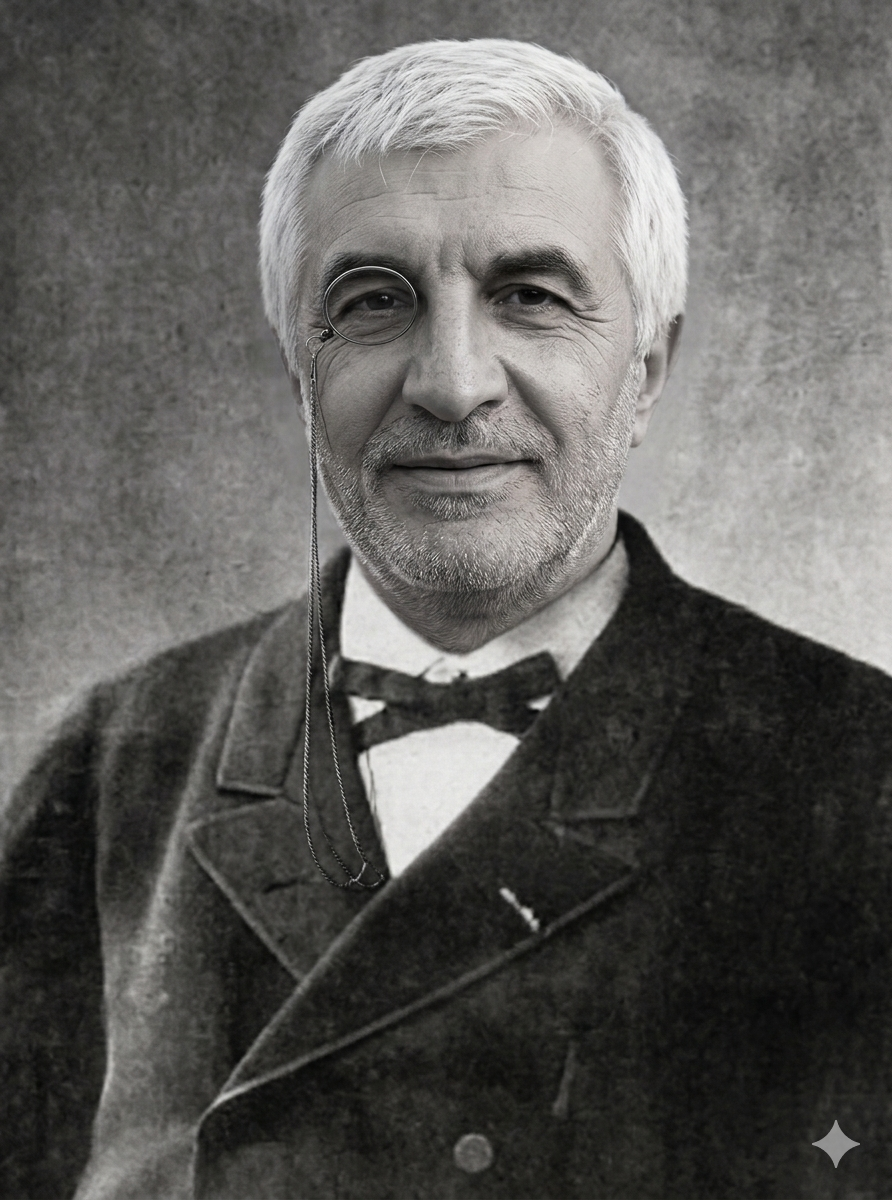
\includegraphics[width=\textwidth]{Immagini/prof_poincare.png}
    \end{minipage}%
    \hspace{0.05\textwidth}% Spazio tra foto e testo
    % Minipage per la citazione (a destra)
    \begin{minipage}{0.65\textwidth}
        \justifying
        \itshape
        "Se noi non fossimo ignoranti non ci sarebbe probabilità, ci potrebbero essere solo certezze. Ma la nostra ignoranza non può essere assoluta, altrimenti non ci sarebbe più probabilità. Così i problemi di probabilità possono essere classificati a seconda della maggiore o minore profondità della nostra ignoranza."
        
        \vspace{1.5em}
        \upshape \hfill --- \textsc{Andrea Bressan} \\
        \hfill \footnotesize \textit{(Sotto mentite spoglie di Henri Poincaré)}
    \end{minipage}
\end{center}
\vspace{2.5em}




\justifying
\newpage 
\begin{center}
\section*{Premessa}
Le sotto sezioni in Rosso sono quelle che riguardano il ripasso di Bressan, tutte le altre (in nero) sono quelle che riguardano il programma dell'anno attuale.    
\end{center}

\tableofcontents
\newpage

\setcounter{section}{-1}
\section{Contatti e informazioni}
\begin{itemize}
    \item Mail: agata.trovato@units.it
    \item Ufficio: Edificio F, primo piano, Aula 114
    \item Ricevimento: Giovedì dalle 14:00 alle 1:00
\end{itemize}

\lezione{\color{red}Introduzione / Ripasso di Bressan}{2025}

La probabilità è la misura del grado della credenza che un certo evento avvenga.

L'oggetto della teoria è un certo \textit{esperimento causale}, la cui esecuzione è detta \textit{prova}, il risultato è indicato con \textit{$\omega$}, l'insieme di
tutti gli $\omega$ possibili è detto \textit{spazio campione $\Omega$}. Un \textit{Evento A} è un sottoinsieme di $\Omega$, se $\omega$ $\in$ A allora esso realizza l'Evento.
Se esso è l'unico elemento costituente di A allora esso è l'\textit{evento elementare}, altrimenti A è un \textit{evento composto}.
Altre nomenclature sono legate alla teoria insiemistica (per esempio due eventi A e B sono disgiunti se l'insieme A non interseca l'insieme B).
\subsection{\color{red} Definizioni di probabilità}
Si possono dare due definizioni di probabilità:
\begin{description}

\item[CLASSICA]: dato uno spazio \textbf{finito} $\Omega$, la probabilità è il rapporto:

\[
P(E)= \frac{\text{casi favorevoli}}{\text{casi possibili}}
\]

Questa funzione è utile quando i casi risultano essere \textbf{ugumente possibili}.

\vspace{0.5cm}

\item[FREQUENTISTICA]: emerge dal ragioanamento fondato sui risultati di un esperimento:
\[
P(E)=\lim_{N \rightarrow \infty} \frac{n}{N}
\]

dove $n$ è il numero di volte che si verifica un evento, mentre N è le volte che viene ripetuto l'esperimento.
\end{description}


\subsection{\color{red} Definizione assiomatica di probabilità}
Dato un evento A $\subseteq \Omega$ la misura di probabilità $P$ è una funzione $P:\Omega \rightarrow \mathbf{R}  $ le cui caratteristiche sono:



\begin{itemize}
    \item $P(A) \geq 0$
    \item $P (evento \hspace{0.1cm} certo)=1$
    \item  Se A e B sono eventi \textbf{disgiunti} (incompatibili), cioè $P(A \cap B) = 0$, allora $P(A \cup B) = P(A)+P(B)$, che nella forma generalizzata risulta essere:
    \[
    P(\bigcup_{i=1}^{\infty}A_i)=\sum_{i=1}^{\infty}P(A_i)
    \]
\end{itemize}

\subsection{\color{red} Proprietà della misura di probabilità}
\begin{itemize}

    \item Probabilità negazione: $P(\overline{A})=1-P(A)$
    \item Estremi della misura di probabilità: $0 \leq P(A)\leq 1$
    \item Teorema delle probabilità totali (con $A \bigcap B \neq 0$): 
    \[
    P(A \cup B)=P(A)+P(B)-P(A \cap B)
    \]
    \[
    P(A - B)=P(B)-P(A \cap B)
    \]
    \item Probabilità in relazione d'inclusione (con $A\subseteq B$): $P(A)\leq P(B)$
\end{itemize}


\subsubsection{\color{red} Probabilità condizionata}

La probabilità che si verifichi $A$ se si verifica $B$: 
\[
P(A|B)=\frac{P(A \bigcap B)}{P(B)}
\]

Il \textbf{Teorema delle probabilità totale} mi enuncia che se ho che se ho n eventi e si ha che 
\[ \displaystyle P(M_i \cap M_j)=0 \hspace{0.3cm}\forall i \neq j \hspace{0.5cm} \& \hspace{0.5cm} \bigcup_{i=0}^{n}M_i=\Omega \]
dove $\Omega$ è lo spazio campione; allora:
\[
P(A)=\sum_{i=1}^{n}P(A|M_i)P(M_i)
\]
Mentre per l'indipendenza si ha $P(A \cap B)=P(A)P(B)$

\subsubsection{\color{red} Probabilità delle cause}
Ci chiediamo quale sia la probabilità che $M_j$ sia la causa di un certo evento $A$.


\subsection{\color{red} Teorema di Bayes }
Dato un certo set di ipotesi ($M_i$) e un certo evento $A$ il teorema mi dice come la probabilità a "posteriori" $P(M_i|A)$ cambia dopo che l'evento $A$ si è verificato.

Consideriamo un eveneto $A$ e una classe completa di ipotesi ($M_j$):
\[
\begin{cases}
    M_i\bigcap M_j=0 \\
    \bigcup_j M_j=\Omega
\end{cases}
\]
 
Utilizzando il teorema della probabilità condizionata e il fatto che $P(A \bigcap M_i)=P(M_i \bigcap A)$ posso ricavare la probabilità che una causa sia dovuta a un determinato evento
\[
P(M_i|A)=\frac{P(A|M_I)P(M_i)}{P(A)}=\frac{P(A|M_i)P(M_i)}{\sum_{j=1}^{n}P(A|M_j)P(M_j)}
\]
Dove:
\begin{description}
    \item[P(M)]: probabilità a priori/margianale (non tiene conto di A)
    \item [P(M \textbar \space A)]: probabilità condizionata/a posteriori, nota A
    \item [P(A \textbar \space M)]: probabità condizionata di A, nota M
    \item [P(A)]: è la probabilità di A a priori, serve da costante di normalizzazione
\end{description}




\subsection{\color{red}Indipendenza}
Si dicono due eventi indipendenti: $P(A \cap B)=P(A) \cdot P(B)$ e quindi $P(A|B)=P(A)$ 

Per esempio: nella misura del pendolo fermare il pendolo ad ogni misura rende le misure indipendenti fra di loro (una misura di un periodo sbagliato non influisce sulla misura successiva).

\subsection{\color{red}Cenni di calcolo combinatorio e fattoriale}
Si chiama combinazione semplice quella in cui non importa l'ordine degli elementi e il numero di combinazioni $C_{n,r}$ è dato da:

\[
C_{n,r} = \binom{n}{r} = \frac{n!}{r!(n - r)!}
\]

Con la definizione di fattoriale:

\[
n! = \prod_{k=1}^{n} k = 1 \cdot 2 \cdot 3 \cdots n = \prod_{i=0}^{n-1} (n - i)
\]

Fattoriale di un numero negativo:
\[
n!=\prod_{i=0}^{n-1}(n-i)
\]
\[
{(c)}^n n!=\prod_{i=0}^{n-1}c(n-i)
\]
\[
{(-1)}^n n!=\prod_{i=0}^{n-1}-1(n-i)=(-n)!
\]

Fattoriale di un numero positivo:
\[
x! = \Pi(x)=\int_{0}^{\infty}t^{x}e^{-t}dt
\]
Che presenta la proprietà:
\[
\Pi(x+1)=(x+1)\Pi(x)
\]

Sempre Eulero introdusse la funzione Gamma $\Gamma$, con uno spostamneto di unità nelle variabili rispetto a $\Pi$:
\[
\Gamma(z)=\int_{0}^{\infty}t^{z-1}e^{-t}dt
\]
Difatti questa funzione è legata a $\Pi$ da $\Pi(x)=\Gamma(x+1)=x\!$ e vale che $z\Gamma(z)=\Gamma(z+1)$

Da questa funzione sono definte le combinazioni semplici del tipo:
\[
\binom{z}{k}=\frac{\Gamma(z+1)}{k\! \Gamma(z-k+1)}
\]

Importanti relazioni tra le funzioni Gamma sono:
\[
\Gamma(z)\Gamma(1-z)=\frac{\pi}{\sin(\pi z)} \hspace{1.5cm} \Gamma(z)\Gamma(-z)=-\frac{\pi}{\sin(\pi z)}
\]
Da queste ricavo che $\Gamma(\frac{1}{2})=\sqrt{\pi}$ e $\Gamma(-\frac{1}{2})=-\sqrt{\pi}$, l'ultima importante relazione è invece:
\[
\Gamma(n+\frac{1}{2})=\frac{(2n-1)!!}{2^n}\sqrt{\pi}
\]







\lezione{Introduzione e Statistica}{6 Ottobre 2025} 
\subsection{Rappresentazione grafica dei dati}
Le nostre misure saranno del tipo ${x_1, x_2, ..., x_N}$, il nostro obiettivo è quello di rappresentare questi dati per capire il fenomeno fisico
che stiamo studiando.\\
Per quanto riguarda la parte grafica, la rappresentazione dipende dai dati a disposizione:
\begin{itemize}
    \item \textbf{Istogramma}: Avendo molte misure di una sola grandezza, la rappresentazione tipica è l'istogramma. Per farlo si divide l'intervallo atteso delle misure in intervalli più piccoli detti \textit{bin}, e si conta quante misure cadono in ogni intervallino.
    \item \textbf{Scatter Plot}: Avendo poche misure di due o più variabili correlate, la rappresentazione più utile è un plot a dispersione (punti $(x,y)$ sul piano cartesiano).
\end{itemize}

\subsubsection{Scatter Plot ed Errori}
L'altra rappresentazione classica è lo scatter plot in cui plottiamo una grandezza rispetto all'altra e aggiungiamo per ogni punto gli errori di misura:
\[ (x_i \pm \sigma_{x_i}, \quad y_i \pm \sigma_{y_i}) \]
In questa rappresentazione è stato usato un numero per rappresentare una misura di $x$ ed è stato associato ad esso una stima dell'errore fatto nella singola misura.

Gli errori da associare dipendono dalla situazione pratica:
\begin{itemize}
    \item In alcuni casi si può fare un'analisi statistica ripetendo le misure molte volte.
    \item Nella maggior parte dei casi  questo non si può fare (strumento non abbastanza sensibile o fenomeno non ripetibile). In tal caso si associa l'errore di sensibilità dello strumento.
\end{itemize}

\subsubsection{Istogramma}

\begin{center}
\begin{tikzpicture}
\begin{axis}[
    ybar,
    enlargelimits=0.15,
    legend style={at={(0.5,-0.15)},
      anchor=north,legend columns=-1},
    ylabel={Frequenza},
    symbolic x coords={A,B,C,D,E},
    xtick=data,
    nodes near coords,
    nodes near coords align={vertical},
]
\addplot coordinates {(A,40) (B,65) (C,52) (D,49) (E,73)};
\addplot coordinates {(A,35) (B,55) (C,45) (D,60) (E,68)};
\legend{Serie 1, Serie 2}
\end{axis}
\end{tikzpicture}
\end{center}


\subsection{Grandezze Statistiche: Media e Varianza}


\ripasso{Valore di Aspettazione}

Le caratteristiche principali delle distribuzioni di probabilità sono descritte attraverso specifici parametri: gli \textit{indici di posizione}, che indicano attorno a quali valori è centrata la distribuzione, e gli \textit{indici di dispersione}, che ne quantificano la "larghezza" o variabilità.
Tra gli indici di posizione, riveste particolare importanza il \textbf{valore di aspettazione}.

Data una variabile casuale $X \in [a,b]$ e la funzione di densità di probabilità $f_X(x)$ ad essa associata, è possibile definire il valore di aspettazione di una generica funzione $g(x)$ come:
\[
E[g(x)]= \int_{a}^{b} g(x) f_X(x) dx \hspace{0.5cm} (\text{caso continuo})
\]
oppure, per il caso discreto:
\[
E[g(x)]=  \sum_{i=1}^{n} g(x_i) p_i
\]
Si tratta, quindi, di una media dei valori assunti da $g(x)$, pesata con la rispettiva densità di probabilità (o probabilità $p_i$).

Il valore di aspettazione gode di proprietà analoghe a quelle di un'applicazione lineare.

Per una variabile casuale continua, il \textbf{valore di aspettazione} di $X$ stesso è dato da:
\[
\mu_x = E[x] = \int_{\Omega}^{} x f_{X}(x) dx
\]
Il parametro $\mu_x$ è definito come \textit{valore medio}. Un ragionamento analogo si applica alle variabili casuali discrete (sostituendo l'integrale con la sommatoria).

Poiché $\mu_x$ è una costante e ha la stessa dimensione fisica della variabile casuale, vale la proprietà:
\[
E[\mu_x] = \mu_x
\]
Esso rappresenta un "indice di posizione" fondamentale all'interno del dominio della variabile.


\subsubsection{Media Aritmetica}

Consideriamo il caso ottimistico in cui si riesce a misurare tante volte la stessa grandezza nelle stesse condizioni. In questo caso, se si vuole usare un solo numero per descrivere le misure, il migliore è senz'altro la \textbf{media aritmetica}:
\begin{equation}
    \bar{x} = \frac{1}{N} \sum_{i=1}^{N} x_i
\end{equation}

\ripasso{Varianza e Deviazione Standard}

Oltre alla media, esistono altri indici di posizione:
\begin{description}
    \item[Moda]: il valore di $x$ in corrispondenza del quale la funzione $f_X(x)$ assume il suo massimo;
    \item[Quantili]: valori associati alla probabilità che la variabile casuale cada in determinati intervalli, definiti tramite la funzione di distribuzione cumulativa:
    \[ \alpha = F(x) = \int_{- \infty}^{x} f(t) dt\]
\end{description}

Considerando la media campionaria $\bar{x}$ definita come $\bar{x} = \frac{1}{N} \sum_{i=1}^{N} x_i$, per definizione la somma degli scarti dalla media deve essere nulla:
\[
\frac{1}{N}\sum_{i=1}^{N} (\bar{x}-x_i)=0
\]

Per ottenere informazioni sulla dispersione dei dati, si definisce la \textbf{varianza} della variabile casuale come la media dei quadrati degli scarti:
\[
var(x)= \frac{1}{N} \sum (x_i - \bar{x})^2
\]

Sviluppando il quadrato all'interno della sommatoria, si ottiene un'espressione utile per i calcoli:
\[
\begin{aligned}
var(x) &= \frac{1}{N} \sum (x_i^2 - 2 \bar{x} x_i + \bar{x}^2) \\
&= \frac{1}{N} \sum x_i^2 - 2 \bar{x} \frac{1}{N} \sum x_i + \frac{1}{N} \sum \bar{x}^2 \\
&= \overline{x^2} - 2\bar{x}^2 + \bar{x}^2 \\
&= \overline{x^2} - \bar{x}^2
\end{aligned}
\]
Ovvero: la varianza è uguale alla media dei quadrati meno il quadrato della media.

La \textbf{deviazione standard} è definita come $\sigma_x = \sqrt{var(x)}$. Tuttavia, data la limitatezza del campione nelle misure reali, si applica spesso la \textit{correzione di Bessel}, definendo la deviazione standard campionaria come:
\[
\sigma_x = \sqrt{\frac{1}{N-1} \sum (x_i - \bar{x})^2}
\]


\subsubsection{Deviazione Standard e correzione di Bessel}
La varianza ha però la scomodità di avere un'unità di misura al quadrato rispetto a $x$. Si preferisce quindi la \textbf{deviazione standard}:
\[ \sigma_N = \sqrt{\text{Var}(x)} \]

\begin{osservazione}[Correzione di Bessel]
La formula sopra è corretta se le misure rappresentano tutta la popolazione. Nella maggior parte dei casi $x_i$ è solo un \textbf{campione}. Per tener conto del bias dovuto all'uso della media campionaria $\bar{x}$ invece della media vera $\mu$, si usa $N-1$ al denominatore:
\begin{equation}
    \sigma = \sqrt{\frac{1}{N-1} \sum_{i=1}^{N} (x_i - \bar{x})^2}
\end{equation}
\end{osservazione}
Questa correzione diventa trascurabile per $N$ grande, ma è fondamentale per piccoli set di dati.


\subsubsection*{Esempio (Python)}
Di seguito mostriamo come calcolare media e deviazione standard (con e senza correzione) simulando delle misure gaussiane, simuliamo $N=100$ misure con due strumenti diversi ($\sigma_1=1$ e $\sigma_2=0.2$).


\begin{lstlisting}[caption={Calcolo di Media e Deviazione Standard}]
import numpy as np
import matplotlib.pyplot as plt

# 1. Simulo N misure di una grandezza fisica (es. corrente)
N = 100
valore_simulato = 8.0 # Valore vero [mA]
# Caso 1: sigma = 1, Caso 2: sigma = 0.2
misure1 = np.random.normal(loc=valore_simulato, scale=1.0, size=N)
misure2 = np.random.normal(loc=valore_simulato, scale=0.2, size=N)

# 2. Calcolo Media
media1 = np.mean(misure1)
print(f"Media Caso 1: {media1:.4f} mA")

# 3. Calcolo Deviazione Standard (ddof=1 applica la correzione di Bessel N-1)
sigma1_corr = np.std(misure1, ddof=1)
print(f"Sigma Corretto (Bessel): {sigma1_corr:.4f}")

# 4. Istogramma
plt.hist(misure1, alpha=0.7, bins=30, edgecolor='black', label='Caso 1')
plt.hist(misure2, alpha=0.7, bins=30, edgecolor='black', label='Caso 2')
plt.xlabel('Misura, I [mA]')
plt.title('Istogramma delle misure ripetute')
plt.legend()
plt.show()
\end{lstlisting}


\begin{figure}[H]
    \centering
    \includegraphics[width=0.8\textwidth]{Immagini/istogramma.png}
    \caption{Istogramma comparativo delle due serie di misure simulate.}
\end{figure}

\subsection{Errore di sensibilità e Propagazione}
\subsubsection{Propagazione degli Errori}
Data una funzione $f(x,y)$ di variabili casuali indipendenti, la varianza si propaga come:
\begin{equation}
    \sigma_f^2 = \left( \frac{\partial f}{\partial x} \right)^2 \sigma_x^2 + \left( \frac{\partial f}{\partial y} \right)^2 \sigma_y^2
\end{equation}

\begin{example}
\textbf{Esempio numerico:} Calcolo dello spazio percorso in un moto uniformemente accelerato \\
Dati: $v = 200 \pm 10 \, m/s$, \quad $a = 12 \pm 2 \, m/s^2$, \quad $t = 6 \, s$ (errore trascurabile).
\[ s =  vt + \frac{1}{2}at^2 = (200 \cdot 6) + \frac{1}{2} \cdot 12 \cdot 6^2 = 1200 + 216 = 1416 \, m \]

Errore associato $\sigma_s$:
\[ \sigma_s^2 = \left( \frac{\partial s}{\partial v} \right)^2 \sigma_v^2 + \left( \frac{\partial s}{\partial a} \right)^2 \sigma_a^2 = (t)^2 \sigma_v^2 + \left(\frac{1}{2}t^2\right)^2 \sigma_a^2 \]
\[ \sigma_s = \sqrt{ 6^2 \cdot 10^2 + (18)^2 \cdot 2^2 } = \sqrt{3600 + 1296} = \sqrt{4896} \approx 70 \, m \]
Risultato: $s = 1416 \pm 70 \, m$.

\end{example}


\ripasso{Errore di sensibilità e distribuzione uniforme}

Si definisce l'errore di sensibilità come la semiampiezza dell'intervallo di risoluzione: $\displaystyle \Delta x = \frac{X_{\max} - X_{\min}}{N}$. Il risultato della misura sarà espresso come $x \pm \Delta x$.

L'interpretazione statistica assume che il "valore vero" della grandezza appartenga a un insieme continuo di possibili valori $x$, ognuno associato a una probabilità $P(x)$. Poiché nel caso continuo la probabilità di un singolo punto è nulla, si utilizza la \textit{densità di probabilità}, tale che:
\[
P(x_1 < X < x_2) = \int_{x_1}^{x_2} P(x) \; dx
\]
La probabilità totale su tutto il dominio deve essere unitaria (condizione di normalizzazione).

Nel caso continuo, il valore di aspettazione $\mu$ e la varianza $\sigma^2$ sono definiti rispettivamente come il baricentro e il momento di inerzia della distribuzione: $\displaystyle \sigma^2 = \int_{X_{\min}}^{X_{\max}}(x - \mu)^2 P(x) dx$.

Se all'interno dell'intervallo di misura tutti i valori sono \textit{equiprobabili}, $P(x)$ segue una \textbf{distribuzione uniforme}:
\[
P(x)=
\begin{cases}
    c , & x \in [X_{\min}, X_{\max}] \\
    0 , & \text{altrimenti}
\end{cases}
\]

Imponendo la condizione di normalizzazione ($\int P(x)dx = 1$), si ricavano i parametri della distribuzione:
\begin{itemize}
    \item L'altezza della distribuzione è $\displaystyle c = \frac{1}{X_{\max} - X_{\min}}$.
    \item Ponendo per comodità l'origine al centro dell'intervallo (semiampiezza $\Delta$), il valore medio è nullo:
    $\displaystyle \mu = \int_{-\Delta}^{+\Delta} x \frac{1}{2 \Delta } dx = 0$.
    \item La deviazione standard risulta essere:
    $\displaystyle \sigma = \sqrt{\int_{-\Delta}^{+\Delta} (x - 0)^2 \frac{1}{2 \Delta } dx} = \sqrt{\frac{\Delta^2}{3}} = \frac{\Delta}{\sqrt{3}}$.
\end{itemize}

\subsubsection{Errore di Sensibilità}
Quando non è possibile ripetere molte volte la misura, associamo alle misure l'errore dovuto alla sensibilità dello strumento. Questo errore si ottiene leggendo il minimo scarto della variabile consentito dallo strumento (risoluzione):
\[ \Delta x = \frac{x_{max} - x_{min}}{2} \]
Questo è l'errore massimo $x \pm \Delta x$. Statisticamente, assumere che il valore vero si trovi in $[x_{min}, x_{max}]$ equivale ad assumere una \textbf{densità di probabilità uniforme} $P(x)$ di larghezza $2\Delta$.
La densità deve essere normalizzata a 1:
\[ \int_{-\Delta}^{\Delta} C \, dx = 1 \implies C(2\Delta) = 1 \implies C = \frac{1}{2\Delta} \]

Quindi:
\[ P(x) = \begin{cases} \frac{1}{2\Delta} & x \in [-\Delta, \Delta] \\ 0 & \text{altrove} \end{cases} \]

Per una distribuzione uniforme tra $[-\Delta, \Delta]$:
\begin{itemize}
    \item Media: $\mu = 0$
    \item Varianza: $\sigma^2 = \int_{-\Delta}^{\Delta} x^2 \frac{1}{2\Delta} dx = \frac{\Delta^2}{3}$
\end{itemize}
Quindi, se si vuole convertire un errore massimo $\Delta$ in una deviazione standard $\sigma$:
\begin{equation}
    \sigma = \frac{\Delta}{\sqrt{3}}
\end{equation}

\section{Metodo dei Minimi Quadrati}
\subsection{Il Principio}

L'obiettivo è dedurre informazioni fisiche dai dati (fit). Partiamo dalle ipotesi:
\begin{enumerate}
    \item Ho effettuato misure $(x_i, y_i)$ dove l'errore su $x$ è trascurabile.
    \item Per ogni $x$ fisso, ho misurato $y$ con incertezza $\sigma_i$.
    \item Esiste una legge $y = f(x; p)$ (dove $p$ sono i parametri).
\end{enumerate}

Il metodo consiste nel minimizzare la somma degli scarti quadratici pesati, detta \textbf{Chi Quadro} $\chi^2$:
\begin{equation}
    \chi^2 = \sum_{i=1}^{N} \left[ \frac{y_i - f(x_i; p)}{\sigma_i} \right]^2
\end{equation}

Minimizzare significa porre le derivate rispetto ai parametri uguali a zero: $\frac{\partial \chi^2}{\partial p} = 0$.

\ripasso{Metodo dei Minimi Quadrati}

Un metodo fondamentale per stimare i parametri di un modello è quello dei \textbf{minimi quadrati}. 
Consideriamo un set di misure $\vec{x}=(x_1, \dots, x_n)$ e i corrispondenti valori osservati $\vec{y}=(y_1, \dots, y_n)$. Si assume che esista una relazione funzionale $f(x; \lambda)$ che lega le variabili, dove $\vec{\lambda} = (\lambda_1, \dots, \lambda_k)$ sono i parametri ignoti da stimare.

Il principio dei minimi quadrati stabilisce che la miglior stima dei parametri è quella che minimizza la somma degli scarti quadratici pesati:
\[
\chi^2 = \sum_{i=1}^{n} w_i \left[ y_i - f(x_i; \vec{\lambda}) \right]^2
\]
Il peso $w_i$ è legato all'incertezza della misura:
\begin{itemize}
    \item Se tutte le misure hanno la stessa incertezza, il termine $w_i$ può essere omesso (o posto uguale a 1).
    \item Se ogni misura ha un'incertezza diversa $\sigma_i$, allora $w_i = \frac{1}{\sigma_i^2}$. In questo caso la quantità minimizzata coincide con la variabile $\chi^2$ (Chi-quadro).
    \item Se le variabili sono correlate, i pesi coinvolgeranno gli elementi della matrice di covarianza inversa.
\end{itemize}

\textbf{Caso particolare: stima di una costante (Media Pesata)}
Se il modello è una costante $y = \lambda$ (cioè cerchiamo il miglior valore unico che rappresenti i dati), minimizzando il $\chi^2$ si ottiene:
\begin{itemize}
    \item Con errori uguali ($\sigma_i = \sigma$): Media aritmetica
    \[ \hat{\lambda} = \frac{1}{n} \sum_{i=1}^n y_i \]
    \item Con errori differenti ($\sigma_i$): Media pesata
    \[ \hat{\lambda} = \frac{\sum_{i=1}^n \frac{y_i}{\sigma_i^2}}{\sum_{j=1}^{n}\frac{1}{\sigma_j^2}} \]
\end{itemize}

\subsection{Fit Lineare ($y = mx + q$)}
Nel caso di funzione lineare $f(x) = mx + q$ e $\sigma_i = \sigma$ costanti, risolvendo il sistema delle derivate parziali $\frac{\partial \chi^2}{\partial m} = 0$ e $\frac{\partial \chi^2}{\partial q} = 0$, si ottengono le stime analitiche:

Definiamo le somme:
\[ S_x = \sum x_i, \quad S_y = \sum y_i, \quad S_{xx} = \sum x_i^2, \quad S_{xy} = \sum x_i y_i \]
\[ D = N S_{xx} - (S_x)^2 \]

Le stime dei parametri sono:
\begin{equation}
    m = \frac{N S_{xy} - S_x S_y}{D}, \qquad q = \frac{S_{xx} S_y - S_x S_{xy}}{D}
\end{equation}

E gli errori associati (tramite propagazione):
\begin{equation}
    \sigma_m = \sqrt{\frac{N \sigma^2}{D}}, \qquad \sigma_q = \sqrt{\frac{\sigma^2 S_{xx}}{D}}
\end{equation}

\subsubsection*{Esempio (Fit Lineare)}
\begin{lstlisting}[caption={Fit Lineare dei Minimi Quadrati}]
# Dati simulati: Moto uniforme s = v*t + s0
t = np.array([0, 1, 2, 3, 4, 5])       # Tempo [s]
s = np.array([2, 17, 27, 37, 47, 63])  # Spazio [mm]
sigma_s = 2                            # Incertezza [mm]
N = len(t)

# Calcolo Somme
Sx = np.sum(t); Sy = np.sum(s)
Sxx = np.sum(t**2); Sxy = np.sum(t * s)

# Calcolo Parametri
D = N * Sxx - Sx**2
m = (N * Sxy - Sx * Sy) / D
q = (Sxx * Sy - Sx * Sxy) / D

print(f"Velocita' (m): {m:.2f} mm/s")
print(f"Posizione init (q): {q:.2f} mm")

# Plot
plt.errorbar(t, s, yerr=sigma_s, fmt='o', label='Dati')
plt.plot(t, m*t + q, label='Fit Lineare')
plt.xlabel('Tempo [s]'); plt.ylabel('Spazio [mm]')
plt.legend(); plt.show()
\end{lstlisting}


\begin{figure}[H]
    \centering
    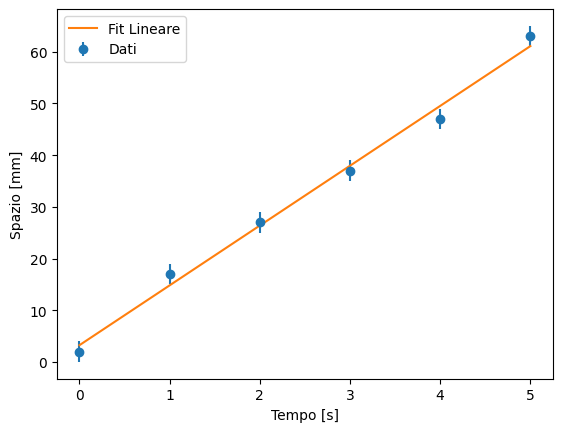
\includegraphics[width=0.8\textwidth]{Immagini/Fit Lineare.png}
    \caption{Fit Lineare}
\end{figure}

\ripasso{Fit di una retta (Regressione Lineare)}

Vogliamo determinare la retta che meglio descrive un set di dati $(x_i, y_i \pm \sigma_i)$.
Utilizziamo la parametrizzazione $f(x) = mx + q$ (oppure $\theta_2 x + \theta_1$), dove i parametri da stimare sono la pendenza $m$ e l'intercetta $q$.
Per trovare il minimo, è necessario risolvere il sistema di equazioni ottenuto annullando le derivate parziali del $\chi^2$:
\[ \frac{\partial \chi^2}{\partial m}=0 \quad \text{e} \quad \frac{\partial \chi^2}{\partial q}=0 \]

\subsubsection*{Caso 1: Errori uguali o trascurabili}
Se gli errori $\sigma_i$ sono tutti uguali, la funzione da minimizzare è:
\[
X^2 = \sum_{i=1}^{N} (y_i - q - m x_i)^2
\]
Introducendo i valori medi $\bar{x}, \bar{y}, \overline{x^2}, \overline{xy}$, le soluzioni per i parametri (stimatori) sono:
\[ 
\begin{split}
q &= \hat{\theta}_1 = \frac{\bar{y} \cdot \overline{x^2} - \bar{x} \cdot \overline{xy}}{\overline{x^2} - \bar{x}^2} \\
m &= \hat{\theta}_2 = \frac{\overline{xy} - \bar{x} \cdot \bar{y}}{\overline{x^2} - \bar{x}^2}
\end{split}
\]
Gli errori sui parametri si ricavano dalla legge di propagazione della varianza (assumendo $\sigma_y = \sigma$ costante per tutti i punti):
\[
\sigma_q^2 = \sigma^2 \frac{\overline{x^2}}{N(\overline{x^2}-\bar{x}^2)}
\quad , \quad
\sigma_m^2 = \sigma^2 \frac{1}{N(\overline{x^2}-\bar{x}^2)}
\]
Nota: Il termine al denominatore $(\overline{x^2}-\bar{x}^2)$ è la varianza dei valori $x_i$ del campione.

\textbf{Caso 2: Errori differenti (Fit pesato)}
Quando ogni misura ha un errore $\sigma_i$ diverso, la probabilità di ottenere il set di misure osservato è data dal prodotto delle probabilità (Likelihood):
\[ P(y_1, \ldots, y_N) \propto \prod_{i=1}^N \exp\left( -\frac{(y_i - q - m x_i)^2}{2\sigma_i^2} \right) = \exp\left( -\frac{1}{2} \sum_{i=1}^N \frac{(y_i - q - m x_i)^2}{\sigma_i^2} \right) \]
Massimizzare questa probabilità equivale a minimizzare l'esponente, ovvero il $\chi^2$:
\[ \chi^2 = \sum_{i=1}^N \frac{(y_i - q - m x_i)^2}{\sigma_i^2} \]
Definiamo le seguenti somme pesate per semplificare la notazione:
\[
S = \sum \frac{1}{\sigma_i^2}, \quad S_x = \sum \frac{x_i}{\sigma_i^2}, \quad S_y = \sum \frac{y_i}{\sigma_i^2}, \quad S_{xx} = \sum \frac{x_i^2}{\sigma_i^2}, \quad S_{xy} = \sum \frac{x_i y_i}{\sigma_i^2}
\]
Definiamo inoltre il determinante del sistema come $\Delta = S \cdot S_{xx} - S_x^2$.
Le migliori stime per i parametri sono:
\[
q = \frac{S_{xx} \cdot S_y - S_x \cdot S_{xy}}{\Delta}
\quad , \quad
m = \frac{S \cdot S_{xy} - S_x \cdot S_y}{\Delta}
\]
Le varianze dei parametri, ottenute tramite la propagazione degli errori, sono:
\[
\sigma_q^2 = \frac{S_{xx}}{\Delta}
\quad , \quad
\sigma_m^2 = \frac{S}{\Delta}
\]
Il valore minimo del $\chi^2$ può essere utilizzato per il \textit{test delle ipotesi} (goodness of fit), per verificare se i dati sono compatibili con l'ipotesi lineare.


\subsection{Caso Non Lineare e Linearizzazione}
se $f(x; p)$ non è lineare spesso si cerca un'espressione linearizzata cambiando variabili.
\\
\\
\textbf{Esempio:} Caduta grave $h = \frac{1}{2}g t^2$ oppure la formula inversa per calcolare $g$ dai tempi:
\[ t = \sqrt{\frac{2}{g}}\sqrt{d} + t_0 \]
Questa equazione è del tipo $Y = mX + q$ se poniamo:
\[ Y = t, \quad X = \sqrt{d}, \quad m = \sqrt{\frac{2}{g}}, \quad q = t_0 \]

Una volta calcolato $\hat{m}$ con i minimi quadrati, inverto la relazione per trovare $g$:
\[ \hat{m}^2 = \frac{2}{g} \implies g = \frac{2}{\hat{m}^2} \]
Per l'errore, uso la propagazione:
\[ \sigma_g = \left| \frac{\partial g}{\partial m} \right| \sigma_m = \left| - \frac{4}{m^3} \right| \sigma_m \]

\subsubsection*{Esempio Computazionale (Linearizzazione)}
\begin{lstlisting}[caption={Linearizzazione per calcolo di g}]
# Dati: Tempo t vs Spazio s
t = np.array([0.16, 0.40, 0.58, 0.72, 0.97]) 
s = np.array([0.20, 1.0, 2.0, 3.0, 5.0])
rad_s = np.sqrt(s) # Variabile linearizzata X

# ... (Codice per calcolo m e q su t vs rad_s omesso per brevita'...)
# Supponiamo m sia stato calcolato:
m_calc = 0.45 
sigma_m = 0.01

# Calcolo fisico
g = 2 / m_calc**2
sigma_g = (4 / m_calc**3) * sigma_m

print(f"g misurato: {g:.2f} +/- {sigma_g:.2f} m/s^2")
\end{lstlisting}




\ripasso{Caso non lineare}
Se la relazione tra le grandezze non è lineare, spesso è possibile "linearizzare" il problema con un cambio di variabile.

\begin{example}
    Consideriamo la legge del moto: $s = \frac{1}{2} g t^2$. 
    Supponiamo di voler misurare $g$ trascurando l'incertezza su $s$ e considerando solo l'errore su $t$.
    Possiamo riscrivere l'equazione come:
    \[ t = \sqrt{\frac{2}{g}} \sqrt{s} \]
    Ponendo $y = t$, $x = \sqrt{s}$ e il parametro $m = \sqrt{\frac{2}{g}}$, otteniamo una relazione lineare $y = mx$ (con intercetta nulla).
    
    Una volta stimato $m$ e la sua varianza $\sigma_m^2$ con il metodo dei minimi quadrati, ricaviamo $g$ invertendo la relazione: $g = \frac{2}{m^2}$.
    L'errore su $g$ si ottiene con la propagazione:
    \[
    \sigma_g = \left| \frac{\partial g}{\partial m} \right| \sigma_m = \left| -\frac{4}{m^3} \right| \sigma_m
    \]
    Questo esempio evidenzia l'importanza della scelta delle variabili dipendenti e indipendenti.
\end{example}

Nei casi in cui la linearizzazione non è possibile, si ricorre all'espansione di Taylor del modello attorno a valori iniziali dei parametri o a metodi numerici iterativi.



\lezione{Momenti e Distribuzioni}{23 Febbraio 2026}



\subsection{Momenti della funzione di distribuzione}



Il valore di aspettazione e la varianza di una variabile casuale sono due particolari “momenti” della funzione densità di probabilità $f_X(x) \equiv f(x)$.

Possiamo distinguere tra momenti calcolati rispetto all’origine e momenti calcolati rispetto al valore di aspettazione (la media). In entrambi i casi, si tratta di valori di aspettazione (dunque quantità numeriche) delle potenze di $x$ o di $x-\mu_x$. 
Nello specifico, definiamo:
   
\begin{definizione} \textbf{Momento algebrico di ordine k} (o k-esimo momento algebrico): calcolato rispetto all'origine.
\[
\mu_k=E[x^k]=\int_\Omega x^k f(x) dx
\]
\end{definizione}

\textbf{Osservazioni:}
\begin{itemize}
    \item Per $k=0 \quad \to \quad  \mu_0 =\int_\Omega f(x) dx =1$ (Normalizzazione della funzione di probabilità).
    \item Per $k=1 \quad \to \quad \mu_1$ rappresenta il valore di aspettazione o media (il baricentro della distribuzione).
\end{itemize}
\begin{definizione}
\textbf{Momenti centrali di ordine k}:
\[
\bar{\mu}_k=E[(x-\mu)^k]=\int_\Omega (x-\mu)^k f(x) dx
\]
\end{definizione}

\textbf{Osservazione:}
\begin{itemize}
    \item Per $\displaystyle k=0 \quad \to \quad \bar{\mu}_0= \int_\Omega f(x) dx = 1$.
    \item Per $k=1 \quad \to \quad \bar{\mu}_1= 0$. \\
    \textit{Dimostrazione:} $\displaystyle \int_\Omega (x-\mu)f(x) dx = \int_\Omega x f(x) dx - \mu \int_\Omega f(x) dx = \mu - \mu \cdot 1 = 0$.
    \item Per $k=2 \quad \to \quad \bar{\mu}_2=\sigma^2$ (Varianza).
    \item Per $k=3 \quad \to \quad \bar{\mu}_3$ è legato all'\textit{indice di asimmetria} (o \textit{skewness}). Esso indica quanto la distribuzione sia simmetrica rispetto alla media:
    \pgfplotsset{
        skewplot/.style={
            width=8cm, height=4cm, 
            axis lines=left,
            xtick=\empty, ytick=\empty, 
            xlabel={$x$},
            ymin=0,
            no markers,
            axis line style={-},
            hide y axis 
        }
    }


    \begin{itemize}
        \item per una distribuzione simmetrica (es. Gaussiana) $\bar{\mu}_3=0$;
         
        \begin{center}
        \begin{tikzpicture}
            \begin{axis}[skewplot, title={Simmetrica ($\bar{\mu}_3=0$)}]
                % Gaussiana
                \addplot[domain=-3:3, samples=60, smooth, thick, RoyalBlue, fill=RoyalBlue!10] {exp(-x^2/2)} \closedcycle;
                % Linea della media
                \draw[dashed, black] (axis cs:0,0) -- (axis cs:0,1) node[above, font=\tiny] {$\mu$};
            \end{axis}
        \end{tikzpicture}
        \end{center}

        \item per una distribuzione asimmetrica a destra (es. Maxwell-Boltzmann) $\bar{\mu}_3>0$;
         \begin{center}
        \begin{tikzpicture}
            \begin{axis}[skewplot, title={Asimmetrica a destra ($\bar{\mu}_3>0$)}]
                % Funzione con coda a destra (simile a Gamma)
                \addplot[domain=0:8, samples=80, smooth, thick, RoyalBlue, fill=RoyalBlue!10] {x^1.8 * exp(-x)} \closedcycle;
                % Nota: Coda lunga verso i valori positivi (destra)
            \end{axis}
        \end{tikzpicture}
        \end{center}

        \item per una distribuzione asimmetrica a sinistra $\bar{\mu}_3<0$
    \begin{center}
        \begin{tikzpicture}
            \begin{axis}[skewplot, title={Asimmetrica a sinistra ($\bar{\mu}_3<0$)}]
                % Speculare alla precedente (coda a sinistra)
                \addplot[domain=-8:0, samples=80, smooth, thick, RoyalBlue, fill=RoyalBlue!10] {(-x)^1.8 * exp(-(-x))} \closedcycle;
                % Nota: Coda lunga verso i valori negativi (sinistra)
            \end{axis}
        \end{tikzpicture}
        \end{center}

    \end{itemize}     

        \item Per $k=4 \quad \to \quad \bar{\mu}_4$ è legato all'\textit{indice di curtosi} (o \textit{kurtosis}). Questo parametro valuta il peso delle "code" della distribuzione, ovvero l'influenza dei valori estremi (\textit{outliers}).

\end{itemize}


\subsection{Distribuzione uniforme discreta}
Consideriamo una variabile $X$ che può assumere $n$ valori discreti. Se tutti i valori sono equiprobabili, imponendo la condizione di normalizzazione si ottiene che la probabilità per ogni valore è $p=1/n$.
Di conseguenza, il valore medio è:
\[
\mu_x=\frac{1}{n}\sum_{i=1}^{n}x_i
\]
che corrisponde alla media aritmetica dei possibili valori (analogo al lancio di un dado).
La varianza è data da:
\[
{\sigma_x}^2=\frac{1}{n} \sum_{i=1}^{n}(x_i-\mu_x)^2
\]


\subsection{Distribuzione uniforme continua}
Una variabile casuale continua definita nell'intervallo $(a,b)$ possiede una distribuzione uniforme se la sua densità di probabilità è costante, ovvero $f_X(x) = \text{cost}$.
Affinché sia soddisfatta la condizione di normalizzazione (l'area sotto la curva deve essere 1), la funzione deve essere:
\[
f_X(x)=\frac{1}{b-a}
\]

Il valore medio si calcola come:
\[
\mu_x=\int_{a}^{b}x f(x) dx = \frac{a+b}{2}
\]


Per la varianza, sfruttando la proprietà $E[x^2]-{E[x]}^2$, si ottiene:
\[
{\sigma_x}^2 = \frac{{(b-a)^2}}{12}
\]


\begin{nota}
    \textbf{Collegamento con la trattazione degli errori.} \\
    Quando si passa dalla teoria degli errori massimi a quella statistica, il risultato di una misura viene espresso come $x \pm \Delta x$. Questo intervallo corrisponde a una distribuzione uniforme di larghezza $b-a = 2\Delta x$.

    Sostituendo nella formula della varianza ricavata sopra ($\sigma_x^2=\frac{(b-a)^2}{12}$), otteniamo la deviazione standard:
    \[
    \sigma_x=\frac{b-a}{2\sqrt{3}} \quad \Rightarrow \quad \Delta x = \sigma_x \sqrt{3}
    \]
    È interessante calcolare la probabilità che il valore $x$ cada all'interno dell'intervallo di una deviazione standard dalla media ($\mu_x \pm \sigma_x$). Tale probabilità risulta essere:
    \[
    P(\mu_x-\sigma_x < x \leq \mu_x + \sigma_x) = \frac{1}{\sqrt{3}} \approx 0.577
    \]
    
    \textit{Dimostrazione:}
    \[
    \int_{\mu_x-\sigma_x}^{\mu_x+\sigma_x} f(x)dx = \frac{1}{b-a}\int_{\mu_x-\sigma_x}^{\mu_x+\sigma_x} dx = \frac{1}{b-a} (2 \sigma_x) = \frac{2\sigma_x}{2\sigma_x\sqrt{3}} = \frac{1}{\sqrt{3}}
    \]
\end{nota}

\vspace{1 cm}




\vspace{1 cm}
\subsection{Funzioni Generatrici e Funzione Caratteristica}
L'introduzione dei momenti risulta utile per diversi motivi. Un risultato fondamentale è il seguente: se due variabili casuali $X$ e $Y$ possiedono gli stessi momenti, allora le loro funzioni di distribuzione di probabilità ($f_X$ e $f_Y$) sono identiche.

\begin{definizione}
    \textbf{Funzione generatrice dei momenti}:
        La funzione generatrice dei momenti, indicata con $M_x(t)$, è definita come il valore atteso di $e^{tx}$. La sua espressione varia a seconda che la variabile casuale sia continua o discreta:
    \[
    M_x(t) = E[e^{tx}] = 
    \begin{cases} 
    \displaystyle \int_\Omega e^{tx}f(x) dx & \text{caso continuo} \\[1em]
    \displaystyle \sum_i p_i e^{tx_i} & \text{caso discreto}
    \end{cases}
    \]
\end{definizione}
Questa funzione è fondamentale perché permette di "generare" i momenti della distribuzione (come media, varianza, ecc.) attraverso l'operazione di derivazione. Calcolando la derivata $m$-esima rispetto a $t$ e valutandola in $t=0$, si ottiene il momento $m$-esimo semplice:

\[
\left[ \frac{\partial ^m M_x}{\partial t^m} \right]_{t=0} = E[x^m] = \mu_m
\]

\paragraph{Dimostrazione:}
Per dimostrare questa proprietà, sviluppiamo $e^{tx}$ in serie di Maclaurin:
\[ 
e^{tx} = \sum_{k=0}^{\infty} \frac{(tx)^k}{k!} 
\]
Sostituendo questo sviluppo nell'integrale della definizione (assumendo il caso continuo per generalità) e sfruttando la linearità dell'integrale, otteniamo:
\[
M_x(t) = \int_\Omega \left( \sum_{k=0}^{\infty} \frac{(tx)^k}{k!} \right) f(x) dx = \sum_{k=0}^{\infty} \frac{t^k}{k!} \int_\Omega x^k f(x) dx 
\]
Poiché l'integrale $\int_\Omega x^k f(x) dx$ corrisponde esattamente al momento $k$-esimo $\mu_k$, possiamo scrivere:
\[
M_x(t) = \sum_{k=0}^{\infty} \frac{t^k}{k!} \mu_k = \mu_0 + \mu_1 t + \frac{\mu_2 t^2}{2!} + \ldots
\]
Se calcoliamo la derivata prima rispetto a $t$:
\[ \frac{\partial M_x}{\partial t} = \mu_1 + \frac{2\mu_2 t}{2!} + \ldots = \mu_1 + \mu_2 t + \ldots \]
Ponendo $t=0$, tutti i termini con $t$ si annullano, lasciando solo il coefficiente $\mu_1$:
\[ \left[ \frac{\partial M_x}{\partial t} \right]_{t=0} = \mu_1 = E[x] \]

\begin{definizione}
    \textbf{Funzione generatrice dei momenti centrali}:
    Analogamente, è possibile definire la funzione che genera i momenti rispetto alla media $\mu$ (momenti centrali):
        \[
    \bar{M}_x(t) = E[e^{t(x-\mu)}] = 
    \begin{cases} 
    \displaystyle \int_\Omega e^{t(x-\mu)}f(x) dx & \text{caso continuo} \\[1em]
    \displaystyle \sum_i p_i e^{t(x-\mu_i)} & \text{caso discreto}
    \end{cases}
    \]
\end{definizione}

Anche in questo caso vale la proprietà delle derivate:
\[
\left[ \frac{\partial ^m \bar{M}_x}{\partial t^m}\right]_{t=0} = E[(x-\mu)^m] = \bar{\mu}_m 
\]


Esiste una relazione diretta tra la funzione generatrice dei momenti semplici e quella dei momenti centrali. Sfruttando le proprietà dell'esponenziale e la linearità del valore atteso, si ha:
\[
\bar{M}_x(t) = E[e^{t(x-\mu)}] = E[e^{tx}e^{-t\mu}] = e^{-t\mu}E[e^{tx}] = e^{-t\mu}M_x(t)
\]


Infine se due variabili casuali $X$ e $Y$ possiedono la stessa funzione generatrice dei momenti ($M_x(t)=M_y(t)$) o la stessa funzione generatrice dei momenti centrali ($\bar{M}_x(t)=\bar{M}_y(t)$), allora le loro distribuzioni di probabilità ($f_X$ e $f_Y$) sono identiche.

\begin{definizione}
    \textbf{Funzione caratteristica}:
    Una variante importante è la funzione caratteristica, definita come:
    \[
    \phi (x) = E[e^{itx}] = \int_\Omega e^{itx}f(x) dx
    \]
    Questa corrisponde formalmente alla \textbf{Trasformata di Fourier} della densità di probabilità.
\end{definizione}
Consideriamo una variabile aleatoria $Z = X + Y$, somma di due variabili aleatorie \textbf{indipendenti} $X$ e $Y$.
La funzione generatrice dei momenti della somma è il prodotto delle singole funzioni generatrici:
\[
M_Z(t) = E[e^{tZ}] = E[e^{t(X+Y)}] = E[e^{tX}e^{tY}]
\]
Essendo $X$ e $Y$ indipendenti, il valore atteso del prodotto è il prodotto dei valori attesi:
\[
M_Z(t) = E[e^{tX}]E[e^{tY}] = M_X(t)M_Y(t)
\]
Questo è dovuto al fatto che $\Omega_X \cap \Omega_Y=0$, dunque vale che $f_{X+Y}(x)=f_X(x) f_Y(x)$

\subsubsection*{Approfondimento sulla funzione caratteristica}
Quella che noi abbiamo visto come i momenti algebrici e centrali, in realtà sono solo due casi particolari di una famiglia più ampia di momenti, 
che possono essere generati da funzioni più generali. La funzione caratteristica è un esempio di funzione generatrice dei momenti che utilizza l'esponenziale complesso $e^{itx}$ invece di $e^{tx}$.\\
La funzione caratteristica è la trasformata della mia p.d.f (probability density function); essa è ben definita valendo $f_X(x) \in L^2[\mathbb{R}]$
\[
\phi(t) = \int_{-\infty}^{\infty} e^{itx} f_X(x) dx = E[e^{itx}]
\]
In questo caso vale la stessa dimostrazione attraverso l'espansione dell'esponenziale per mostrare come da questa si possono ricavare i momenti, dove i momenti sono definiti come:
\[
E[x^m]= \mu_m = \left[ \frac{\partial ^m \phi(t)}{\partial {(it)}^m}\right]_{t=0}
\]
La funzione caratteristica è particolarmente utile perché, essendo la trasformata di Fourier della p.d.f., permette di ricavare la distribuzione di probabilità a partire dalla funzione caratteristica stessa tramite la trasformata inversa di Fourier:
\[
f_X(x) = \frac{1}{2\pi} \int_{-\infty}^{\infty} e^{-itx} \phi(t) dt
\]
Dunque due distribuzioni di probabilità che hanno gli stessi momenti (dunque la stessa funzione caratteristica), sono la stessa distribuzione di probabilità. 
Questo è dovuto al fatto che la $\mathcal{F}$-trasformata in $L^2[\mathbb{R}]$ rappresenta una biezione tra due spazi.
\subsection{Distribuzione binomiale o di Bernoulli}
\emph{Questa parte è stata integrata con gli appunti di Bressan}
\vspace{0.4 cm}

La distribuzione binomiale descrive un fenomeno che può verificarsi solo con due modalità mutualmente esclusive: successo (con probabilità $p$) o insuccesso (con probabilità $q=1-p$).

Se ripetiamo l'esperimento $n$ volte, la probabilità di ottenere esattamente $k$ successi è data dalla funzione:
\[
P(k;n,p) = \binom{n}{k}p^k q^{n-k} = \frac{n!}{k!(n-k)!}p^k (1-p)^{n-k}
\]
Casi particolari immediati:
\begin{itemize}[itemsep=0.1em]
 \item Probabilità di $n$ successi (tutti): $p^n$ 
 \item Probabilità di $0$ successi (nessuno): $q^n$  
 \item Probabilità di $1$ successo: $n p q^{n-1}$ (nota: il coefficiente binomiale $\binom{n}{1}=n$)
 \item Probabilità di $n-1$ successi: $n p^{n-1}q$
\end{itemize}

\begin{example}
    Consideriamo 3 oggetti ($n=3$) chiamati A, B, C. Vogliamo sceglierne 2 ($k=2$). 
    Le possibili combinazioni sono: AB, BC, AC.
    Calcolando con la formula del coefficiente binomiale otteniamo conferma:
    \[
    \binom{3}{2} = \frac{3!}{2!(3-2)!} = \frac{3 \cdot 2 \cdot 1}{2 \cdot 1 \cdot 1} = 3
    \]
\end{example}

\subsubsection*{Proprietà della distribuzione binomiale}
\begin{itemize}
    \item \textbf{Normalizzazione}: La somma di tutte le probabilità è 1. Questo deriva dallo sviluppo del binomio di Newton:
    \[ \sum_{k=0}^{n} \binom {n}{k}p^kq^{n-k} = (p+q)^n = (1)^n = 1 \]
    
    \item \textbf{Calcolo diretto della media}: Possiamo derivare la media manipolando la sommatoria. Derivando l'identità $(p+q)^n$ rispetto a $p$:
    \[
    p \frac{\partial}{\partial p} (p + q)^n = p \cdot n(p+q)^{n-1} \quad \xrightarrow{p+q=1} \quad np
    \]
    Dall'altro lato della sommatoria:
    \[
    p \frac{\partial}{\partial p} \sum_{k=0}^{n} \binom{n}{k} p^k q^{n-k} = \sum_{k=0}^{n} k \binom{n}{k} p^k p^{-1} q^{n-k} \cdot p = \sum_{k=0}^{n} k \binom{n}{k} p^k q^{n-k} = E[k]
    \]
    Uguagliando i risultati otteniamo il valore atteso: $E[k] = np$.
    
    \item \textbf{Varianza}: La varianza è data da $\sigma_x^2 = E[x^2] - E[x]^2 = npq$.
\end{itemize}

\subsubsection*{Funzione generatrice dei momenti della Binomiale}
Calcoliamo il momento generatore per la binomiale:
\[
M_k(t) = E[e^{tk}] = \sum_{k=0}^{n} e^{tk} \binom{n}{k} p^k q^{n-k} = \sum_{k=0}^{n} \binom{n}{k} (pe^t)^k q^{n-k}
\]
Riconoscendo la forma del binomio di Newton $(a+b)^n$ con $a=pe^t$ e $b=q$, otteniamo:
\[
M_k(t) = (pe^t + q)^n
\]

Da qui possiamo ricalcolare i momenti derivando rispetto a $t$:

\begin{enumerate}
    \item \textbf{Valore atteso (Media)}:
    Calcoliamo la derivata prima:
    \[ M'_k(t) = n(pe^t+q)^{n-1} \cdot pe^t \]
    Ponendo $t=0$ (ricordando che $e^0=1$ e $p+q=1$):
    \[ \mu = M'_k(0) = n(p+q)^{n-1}p = np \]

    \item \textbf{Varianza}:
    Calcoliamo la derivata seconda (regola del prodotto):
    \[ M''_k(t) = n(n-1)(pe^t+q)^{n-2}(pe^t)^2 + n(pe^t+q)^{n-1}pe^t \]
    Ponendo $t=0$:
    \[ E[x^2] = M''_k(0) = n(n-1)p^2 + np \]
    Ora calcoliamo la varianza usando $Var(x) = E[x^2] - E[x]^2$:
    \[
    \sigma^2 = [n(n-1)p^2 + np] - (np)^2 = n^2p^2 - np^2 + np - n^2p^2 = np - np^2 = np(1-p) = npq
    \]

    \item \textbf{Asimmetria (Terzo momento centrale)}:
    Il terzo momento centrale è $\bar{\mu_3} = npq(1-2p)$. Questo indice ci dice la forma della distribuzione:
    \begin{itemize}
        \item Se $\bar{\mu_3} > 0$: distribuzione \textbf{asimmetrica positiva} (coda a destra).
        \item Se $\bar{\mu_3} = 0$: distribuzione \textbf{simmetrica}.
        \item Se $\bar{\mu_3} < 0$: distribuzione \textbf{asimmetrica negativa} (coda a sinistra).
    \end{itemize}
\end{enumerate}

\vspace{0.5cm}

\paragraph{Limiti della Binomiale:}
La distribuzione binomiale è estremamente importante in fisica perché, al limite per $n \to \infty$, approssima altre distribuzioni fondamentali:
\begin{itemize}
    \item Tende alla \textbf{distribuzione di Gauss} se $p$ rimane costante.
    \item Tende alla \textbf{distribuzione di Poisson} se il prodotto $np$ rimane costante (ovvero se $p \to 0$ mentre $n \to \infty$).
\end{itemize}

\paragraph{Applicazione agli istogrammi:}
Consideriamo un istogramma dove $n$ è il numero totale di eventi e ci focalizziamo su un particolare intervallo (bin) $i$.
Il numero atteso di eventi in quell'intervallo è $E[n_i] = n p_i$.

La varianza del numero di eventi nell'intervallo è data dalla binomiale:
\[ \sigma_{n_i}^2 = n p_i (1 - p_i) = n_i (1 - p_i) \simeq n_i \left(1 - \frac{n_i}{n}\right) \]
Se stimiamo la probabilità $p_i$ tramite i dati misurati come $\hat{p_i} = n_i^{mis}/n$, nel caso in cui la probabilità sia molto piccola ($p \to 0$, regime di Poisson), il termine $(1-p_i) \approx 1$.
Di conseguenza, l'errore standard (deviazione standard) sul conteggio di un bin è approssimabile con la radice quadrata del conteggio stesso:
\[ \sigma_{n_i} \approx \sqrt{n_i^{mis}} \]

\lezione{Distribuizione di Poisson e Approsimazioni}{26 Febbraio 2026}

\subsection*{Esempi Python: La Distribuzione Binomiale}

In questo esercizio simuliamo il lancio di una moneta per applicare la distribuzione binomiale.
\textbf{Problema:} Lanciamo una moneta $n=10$ volte. Qual è la probabilità di ottenere esattamente $k=6$ teste?

Poiché una moneta può dare testa o croce, la probabilità di successo (testa) è $p=0.5$. Utilizzeremo la distribuzione binomiale con i parametri:
\begin{itemize}
    \item $n = 10$ (numero di lanci)
    \item $k = 6$ (numero di successi richiesti)
    \item $p = 0.5$ (probabilità singolo evento)
\end{itemize}

\subsubsection*{1. Calcolo Analitico e con Librerie}
Possiamo calcolare la probabilità sia implementando la formula matematica, sia utilizzando la libreria \texttt{scipy}.

\begin{lstlisting}[language=Python, frame=single, caption=Calcolo probabilità Binomiale]
import math
from scipy.stats import binom

# Parametri del problema
k = 6
n = 10
p = 0.5

# METODO 1: Formula matematica
# P = coeff_binomiale * (p^k) * ((1 - p)^(n - k))
coeff_binomiale = math.comb(n, k)
P = coeff_binomiale * (p**k) * ((1 - p)**(n - k))

print(f"Probabilita' (formula): {P}")

# METODO 2: Libreria Scipy
# Esiste una funzione dedicata per ottenere lo stesso risultato
P_scipy = binom.pmf(k, n, p)

print(f"Probabilita' (scipy): {P_scipy}")
\end{lstlisting}

Il risultato ottenuto è circa $0.205$. Questo significa che, se ripetiamo molte volte l'esperimento dei 10 lanci, nel $\approx 20\%$ dei casi otterremo esattamente 6 teste.

\subsubsection*{2. Simulazione Monte Carlo}
Possiamo verificare il risultato teorico simulando l'esperimento più volte.
Prima simuliamo un singolo set di 10 lanci, poi ripetiamo l'esperimento 100 volte per contare la frequenza del risultato "6 teste".

\begin{lstlisting}[language=Python, frame=single, caption=Simulazione dei lanci]
import random

# --- Parte A: Singola simulazione di 10 lanci ---
testa = 0
croce = 0
for i in range(10):
    lancio = random.randint(0, 1) # 0 = Testa, 1 = Croce
    if lancio == 0:
        testa += 1
    else:
        croce += 1
print(f"Esito singolo: {testa} Teste e {croce} Croci")

# --- Parte B: Ripetiamo l'esperimento 100 volte ---
testa_l = [] # Lista per salvare i risultati di ogni esperimento

for i in range(100): # 100 esperimenti totali
    testa = 0 # Azzero il contatore per il nuovo esperimento
    for j in range(10): # Ogni esperimento consiste in 10 lanci
        lancio = random.randint(0, 1)
        if lancio == 0:
            testa += 1
    # Fine dei 10 lanci, salvo il risultato
    testa_l.append(testa)

# Contiamo quante volte e' uscito esattamente 6
risultato = testa_l.count(6)
print(f"Su 100 esperimenti, ho ottenuto 6 teste {risultato} volte")
\end{lstlisting}



\subsection{Dalla Binomiale alla Poissoniana}

\ripasso{Distribuzione di Poisson}
La distribuzione di Poisson è un caso limite fondamentale, spesso utilizzato in fisica nucleare, e serve per indicare la probabilità di osservare $k$ eventi in un determinato intervallo di tempo $t$, basandosi su tre ipotesi principali:
\begin{itemize}
    \item \textbf{Indipendenza:} la presenza o assenza di un evento non dipende da ciò che è accaduto prima del tempo $t$ (processo senza memoria).
    \item \textbf{Proporzionalità:} la probabilità che accada un evento in un intervallo infinitesimo $dt$ è proporzionale all'ampiezza dell'intervallo stesso.
    \item \textbf{Non simultaneità:} la probabilità di avere due eventi contemporaneamente in un intervallo infinitesimo è nulla.
\end{itemize}

Si tratta del caso limite della distribuzione binomiale in cui la probabilità di successo $p$ è molto piccola e il numero di prove $n \rightarrow \infty$. La formula generale è:
\[
    P_k(t)=\frac{(\mu t)^k}{k!}e^{-\mu t}
\]
dove $\mu$ rappresenta il tasso medio di eventi per unità di tempo.

\subsubsection*{Derivazione della formula}

\textbf{1. Probabilità di 0 eventi:} \\
Consideriamo la probabilità di non avere eventi nell'intervallo $(0, t+dt)$. Questo richiede che non ci siano eventi fino a $t$ e che non se ne verifichino nell'intervallo successivo $dt$:
\[
P_0(t+dt)=P_0(t)(1-\mu dt)
\]
Qui abbiamo imposto che la probabilità di avere un evento in $dt$ sia $\mu dt$ (e quindi di non averne è $1-\mu dt$, trascurando termini di ordine superiore). Riorganizzando i termini e passando al limite per $dt \to 0$:
\[
\frac{P_0(t+dt) - P_0(t)}{dt} = -\mu P_0(t) \quad \Rightarrow \quad \frac{dP_0}{dt} = -\mu P_0(t)
\]
Imponendo la condizione iniziale $P_0(0)=1$, la soluzione è:
\[
P_0(t)=e^{-\mu t}
\]

\textbf{2. Probabilità di $k$ eventi:} \\
La probabilità di avere 1 evento al tempo $t+dt$ è data dalla somma di due possibilità: avere 1 evento a $t$ e nessuno in $dt$, oppure avere 0 eventi a $t$ e uno in $dt$:
\[
P_1(t+dt)=P_1(t)(1-\mu dt) + P_0(t)(\mu dt)
\]
Che porta all'equazione differenziale:
\[
\frac{dP_1}{dt}=- \mu (P_1(t)-P_0(t))
\]
Procedendo in maniera ricorsiva, si trova che la probabilità di avere $m$ eventi varia secondo:
\[
\frac{dP_m}{dt}=- \mu (P_m(t)-P_{m-1}(t))
\]
La soluzione generale di questo sistema è:
\[
P_k(t)=\frac{(\mu t)^k}{k!}e^{-\mu t}=\frac{m^k}{k!}e^{-m}
\]
dove abbiamo posto $m=\mu t=E[k]$, che rappresenta il valore di aspettazione (il numero medio) di eventi nell'intervallo $t$.

\subsubsection*{Proprietà della distribuzione}
La distribuzione di Poisson è correttamente normalizzata. Infatti, ricordando lo sviluppo di Taylor dell'esponenziale:
\[
\sum_{k=0}^{\infty}P_k = e^{-m} \sum_{k=0}^{\infty}\frac{m^k}{k!} = e^{-m} \cdot e^m = 1
\]
Il valore di aspettazione è:
\[
E[k]=\sum_{k=0}^{\infty}k P_k = m 
\]
E la varianza coincide con la media:
\[
{\sigma^2}=E[k^2]-{E[k]}^2=m
\]
Si nota dunque che la distribuzione di Poisson non è altro che il limite per $n \rightarrow \infty$ della distribuzione di Bernoulli (Binomiale).

\subsubsection{Confronto: Poisson vs Binomiale}
La distribuzione \textbf{Binomiale} descrive casi in cui un risultato particolare si ottiene in un numero preciso e finito di tentativi ($n$).

La distribuzione di \textbf{Poisson}, invece, si usa per descrivere casi in cui si contano eventi rari in un continuo (tempo o spazio), dove non si ha un'idea precisa del numero di tentativi totali, né ha senso parlare di casi "sfavorevoli" nel senso classico.

\textbf{Esempi:}
\begin{itemize}
    \item Il numero di fulmini durante un temporale: sarà un numero intero, ma non ha senso parlare di "non-fulmini" (non esiste un non-evento osservabile come nel caso "Testa o Croce").
\end{itemize}
In questi processi si vuole stimare la probabilità $k$ di eventi, noto il numero medio $\lambda$ (o $\mu$) di eventi che generalmente si presentano. Il processo non ha memoria: un evento verificatosi non influenza la probabilità dei successivi.

\subsubsection*{Dimostrazione del limite}
Matematicamente, la Poisson si ottiene dalla Binomiale attraverso i limiti:
\[
n \to \infty \quad \text{e} \quad p \to 0
\]
in modo tale che il loro prodotto $\lambda = np$ rimanga costante ($\lambda = \text{cost}$).

Supponiamo di attenderci $\lambda$ eventi in un certo intervallo di tempo $\Delta t$. Dividiamo questo intervallo in $n$ sotto-intervalli $\Delta t'$ molto piccoli ($n \to \infty$), talmente piccoli che la probabilità che due eventi cadano nello stesso sia trascurabile (al massimo un evento per intervallo).
La probabilità che un evento si verifichi in un singolo $\Delta t'$ è:
\[
p = \frac{\lambda}{n}
\]
La probabilità di trovare $k$ eventi negli $n$ intervallini è data dalla distribuzione Binomiale con $p = \lambda/n$:
\[
P\left(k; n, \frac{\lambda}{n}\right) = \binom{n}{k} p^k (1-p)^{n-k} = \frac{n!}{k!(n-k)!} \left(\frac{\lambda}{n}\right)^k \left(1 - \frac{\lambda}{n}\right)^{n-k}
\]
Riorganizziamo i termini per calcolare il limite:
\[
P\left(k; n, \frac{\lambda}{n}\right) = \frac{\lambda^k}{k!} \cdot \underbrace{\frac{n!}{(n-k)! \, n^k}}_{(A)} \cdot \underbrace{\left(1 - \frac{\lambda}{n}\right)^{n-k}}_{(B)}
\]

\textbf{1. Il termine fattoriale (A):}
\[
\frac{n!}{(n-k)!} = n \cdot (n-1) \cdot (n-2) \cdots (n-k+1)
\]
Ci sono esattamente $k$ termini al numeratore. Per $n \to \infty$, possiamo trascurare le sottrazioni rispetto a $n$ (es. $n-1 \approx n$). Quindi:
\[
\lim_{n \to \infty} \frac{n!}{(n-k)!} \approx \underbrace{n \cdot n \cdots n}_{k \text{ volte}} = n^k
\]
(Esempio con $k=5$: $\frac{n(n-1)(n-2)(n-3)(n-4)}{1} \to n^5$).
Di conseguenza, il rapporto tende a 1:
\[
\lim_{n \to \infty} \frac{n!}{(n-k)! \, n^k} = \frac{n^k}{n^k} = 1
\]

\textbf{2. Il termine esponenziale (B):}
Scriviamo il termine $\left(1 - \frac{\lambda}{n}\right)^{n-k}$ come prodotto di due fattori:
\[
\left(1 - \frac{\lambda}{n}\right)^{n} \cdot \left(1 - \frac{\lambda}{n}\right)^{-k}
\]
Per $n \to \infty$, il secondo fattore tende a $(1-0)^{-k} = 1$.
Il primo fattore è un limite notevole dell'analisi matematica:
\[
\lim_{n \to \infty} \left(1 + \frac{x}{n}\right)^n = e^x \implies \lim_{n \to \infty} \left(1 - \frac{\lambda}{n}\right)^n = e^{-\lambda}
\]

Sostituendo i limiti calcolati ($n \to \infty, p \to 0, np=\lambda$) nell'espressione della binomiale, otteniamo la forma chiusa della distribuzione.
La probabilità di ottenere $k$ eventi, dato un numero medio di eventi attesi $\lambda$, è:
\begin{equation}
\boxed{P(k; \lambda) = \frac{e^{-\lambda} \lambda^k}{k!} \quad \text{con } 0 \le k < \infty}
\end{equation}
\textbf{Condizioni di validità:} Il modello è valido per eventi rari in un continuo, dove il numero di prove tende all'infinito.
Un esempio classico è il \textbf{decadimento radioattivo}, in quanto il numero di decadimenti nucleari in un intervallo di tempo è discreto e casuale, ma con un tasso medio ben definito.


\subsection{Calcolo dei Momenti tramite la Funzione Generatrice dei Momenti}
Per calcolare valore atteso e varianza in modo elegante, utilizziamo la \textbf{Funzione Generatrice dei Momenti}, definita come il valore atteso di $e^{tk}$:
\[
M_k(t) = E[e^{tk}] = \sum_{k=0}^{+\infty} e^{tk} P(k; \lambda) = \sum_{k=0}^{+\infty} e^{tk} \frac{e^{-\lambda} \lambda^k}{k!}
\]
Portiamo fuori dalla sommatoria i termini costanti rispetto a $k$ (il termine $e^{-\lambda}$) e accorpiamo le potenze di $k$:
\[
M_k(t) = e^{-\lambda} \sum_{k=0}^{+\infty} \frac{(e^t \lambda)^k}{k!}
\]
Riconosciamo nella sommatoria lo sviluppo in serie di Taylor dell'esponenziale $e^x = \sum_{n=0}^{\infty} \frac{x^n}{n!}$, dove in questo caso l'argomento è $x = \lambda e^t$.
\[
M_k(t) = e^{-\lambda} \cdot e^{(\lambda e^t)} = e^{\lambda e^t - \lambda}
\]
Possiamo quindi scrivere la forma finale della Funzione Generatrice dei Momenti per la Poissoniana:
\begin{equation}
\boxed{M_k(t) = e^{\lambda(e^t - 1)}}
\end{equation}

\subsubsection*{Calcolo di Media e Varianza}
Dalle proprietà della Funzione Generatrice dei Momenti sappiamo che la derivata prima valutata in $t=0$ fornisce la media, mentre la derivata seconda fornisce il momento secondo.

\paragraph{1. Media (Valore Atteso):}
Deriviamo $M_k(t)$ rispetto a $t$:
\[
\frac{\partial M_k}{\partial t} = \frac{\partial}{\partial t} \left( e^{\lambda(e^t - 1)} \right) = e^{\lambda(e^t - 1)} \cdot \frac{\partial}{\partial t}(\lambda e^t - \lambda) = e^{\lambda(e^t - 1)} \cdot \lambda e^t
\]
Valutiamo in $t=0$:
\[
E[k] = \left[ \frac{\partial M_k}{\partial t} \right]_{t=0} = e^{\lambda(1-1)} \cdot \lambda \cdot 1 = 1 \cdot \lambda = \lambda
\]
\textbf{Risultato:} $\mu = \lambda$. Questo conferma che il parametro $\lambda$ rappresenta il numero medio di eventi.

\paragraph{2. Varianza:}
Per la varianza usiamo la relazione $\text{Var}(k) = E[k^2] - (E[k])^2$.
Calcoliamo la derivata seconda (derivata del prodotto $f(t) \cdot g(t)$ dove $f$ è l'esponenziale composto e $g$ è $\lambda e^t$):
\[
\frac{\partial^2 M_k}{\partial t^2} = \frac{\partial}{\partial t} \left( \underbrace{e^{\lambda(e^t - 1)}}_{f(t)} \cdot \underbrace{\lambda e^t}_{g(t)} \right)
\]
\[
= \underbrace{e^{\lambda(e^t - 1)} \lambda e^t}_{f'(t)} \cdot \lambda e^t + \underbrace{e^{\lambda(e^t - 1)}}_{f(t)} \cdot \underbrace{\lambda e^t}_{g'(t)}
\]
Raccogliendo i termini:
\[
\frac{\partial^2 M_k}{\partial t^2} = e^{\lambda(e^t - 1)} (\lambda^2 e^{2t} + \lambda e^t)
\]
Valutando in $t=0$:
\[
E[k^2] = 1 \cdot (\lambda^2 + \lambda) = \lambda^2 + \lambda
\]
Ora calcoliamo la varianza sottraendo il quadrato della media:
\[
\text{Var}(k) = (\lambda^2 + \lambda) - (\lambda)^2 = \lambda
\]

\textbf{Conclusione:} Per la distribuzione di Poisson, media e varianza coincidono.
\begin{equation}
\boxed{\mu = \lambda, \quad \sigma^2 = \lambda}
\end{equation}

\subsection{Relazione con la Binomiale e Somma di Variabili}

\subsubsection{Limite della Funzione Generatrice dei Momenti Binomiale}
Si può dimostrare formalmente che la Funzione Generatrice della Binomiale tende a quella della Poissoniana.
La Funzione Generatrice dei Momenti della Binomiale è $M_{bin}(t) = (pe^t + 1 - p)^n = [1 + p(e^t - 1)]^n$.
Sostituendo $p = \lambda/n$:
\[
M_{bin}(t) = \left[ 1 + \frac{\lambda(e^t - 1)}{n} \right]^n
\]
Utilizzando il limite notevole $\lim_{n \to \infty} (1 + \frac{a}{n})^n = e^a$ con $a = \lambda(e^t - 1)$, otteniamo:
\[
\lim_{n \to \infty} M_{bin}(t) = e^{\lambda(e^t - 1)}
\]
Che è esattamente la Funzione Generatrice dei Momenti della Poissoniana derivata in precedenza.

\subsubsection{Confronto delle forme (Code della distribuzione)}
\begin{itemize}
    \item \textbf{Varianza:} La varianza della Poissoniana è $\lambda = np$. La varianza della Binomiale è $np(1-p)$.
    Poiché $(1-p) < 1$, la varianza binomiale è sempre minore di quella Poissoniana equivalente.
    \item \textbf{Code:} La distribuzione binomiale è limitata superiormente ($k \le n$). La Poissoniana non ha limite superiore ($0 \le k < \infty$). Questo, unito alla varianza maggiore, implica che la Poissoniana ha \textbf{code più lunghe}: è relativamente più probabile osservare valori lontani dalla media rispetto a una binomiale, specialmente quando la media è piccola.
\end{itemize}

\subsubsection{Somma di Poissoniane Indipendenti}
Se abbiamo due processi Poissoniani indipendenti $A$ e $B$ con medie $\lambda_a$ e $\lambda_b$, la variabile somma $k = k_a + k_b$ segue ancora una distribuzione di Poisson con media $\lambda_{tot} = \lambda_a + \lambda_b$.

\textbf{Dimostrazione:} La Funzione Generatrice dei Momenti della somma di variabili indipendenti è il prodotto delle Funzione Generatrice dei Momenti.
\[
M_{tot}(t) = M_a(t) \cdot M_b(t) = e^{\lambda_a(e^t - 1)} \cdot e^{\lambda_b(e^t - 1)} = e^{(\lambda_a + \lambda_b)(e^t - 1)}
\]
Questa forma corrisponde a una Poissoniana con parametro $\lambda_a + \lambda_b$.
\textit{Esempio fisico:} Un contatore Geiger che rileva radiazioni da due sorgenti diverse non distinguibili; il conteggio totale sarà ancora Poissoniano.

\subsection*{Esempi Python: Grafici e Confronti}

Di seguito riportiamo il codice per visualizzare le distribuzioni e verificare numericamente le proprietà discusse.

\subsubsection*{1. Visualizzazione della Distribuzione Binomiale}
Questo script mostra come varia la forma della distribuzione binomiale al variare di $n$ (numero di prove) e $p$ (probabilità).

\begin{lstlisting}[language=Python, frame=single, caption={Plot della Binomiale al variare di n e p}]
import math
from matplotlib import pyplot as plt
import numpy as np

def binomiale_manual(k, n, p):
    return math.comb(n, k) * (p**k) * ((1 - p)**(n - k))

# Creiamo una matrice di grafici 2x2 per vedere diversi n
fig, axes = plt.subplots(2, 2, figsize=(8, 6))
axes = axes.flatten()

n_list = [5, 15, 30, 50]
p = 0.5

for ax, n in zip(axes, n_list):
    k_values = range(n + 1)
    P_binom = [binomiale_manual(k, n, p) for k in k_values]
    ax.bar(k_values, P_binom)

    # Linee per media e deviazione standard
    mu = n * p
    sigma = np.sqrt(n * p * (1 - p))
    
    ax.axvline(mu, linestyle="--", color="orange", label=f"$\mu$={mu:.1f}")
    y_lvl = max(P_binom)/2
    ax.plot([mu-sigma, mu+sigma], [y_lvl, y_lvl], color="red", label=f"$\sigma$={sigma:.1f}")

    ax.set_title(f"n={n}, p={p}")
    ax.legend()
    ax.grid(True)

plt.tight_layout()
plt.show()
\end{lstlisting}

\begin{figure}[H]
    \centering
    
    \begin{subfigure}[b]{0.45\textwidth}
        \centering
        
        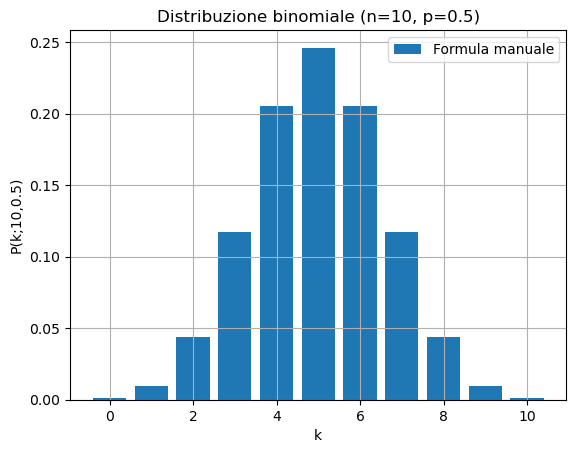
\includegraphics[width=\textwidth]{Immagini/Binomiale n=10 p=0.5.png} 
        \caption{}
        \label{fig:img1}
    \end{subfigure}
    \hfill 
    \begin{subfigure}[b]{0.45\textwidth}
        \centering
        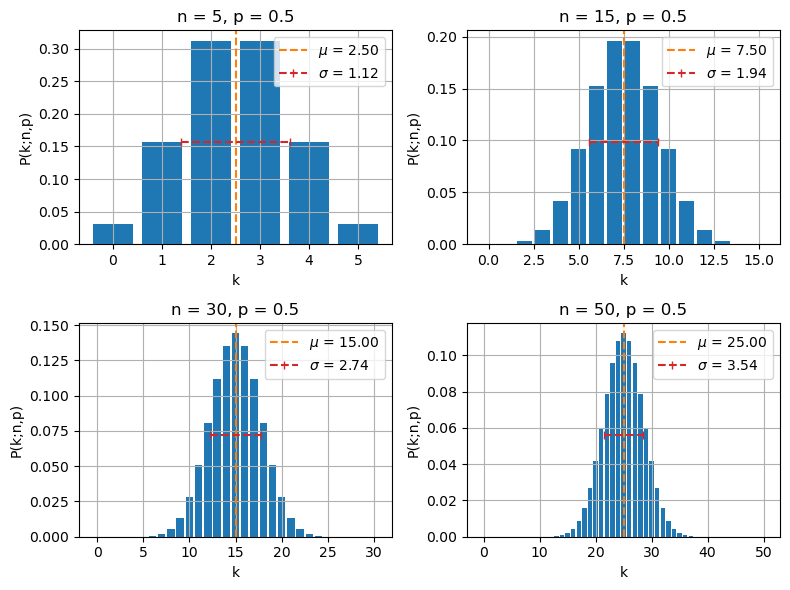
\includegraphics[width=\textwidth]{Immagini/binomiale con diversi p e n.png}
        \caption{}
        \label{fig:img2}
    \end{subfigure}
    
    \vspace{1cm} 
    
    \begin{subfigure}[b]{0.8\textwidth}
        \centering
        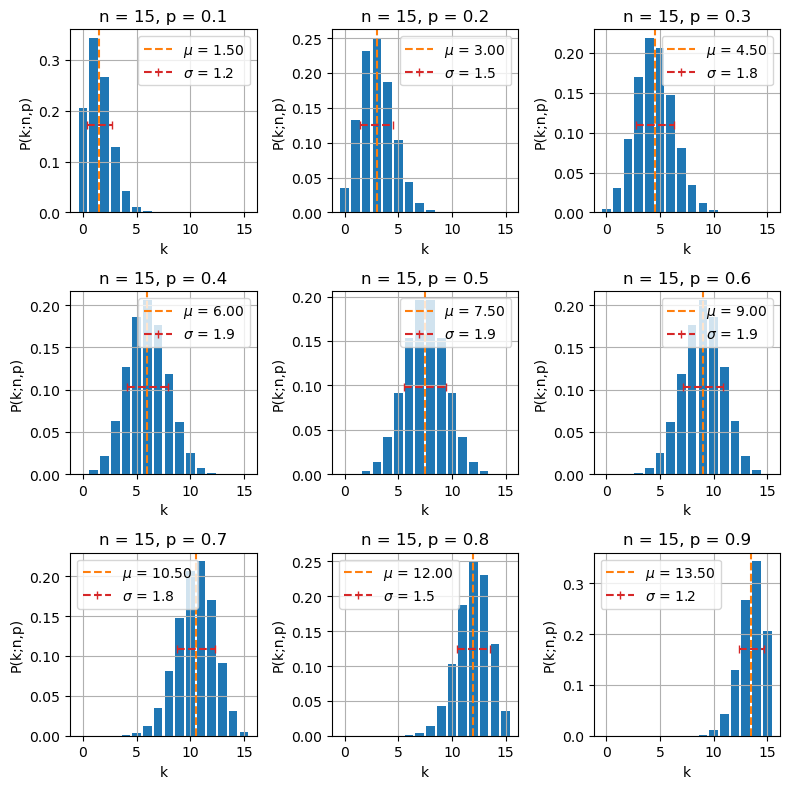
\includegraphics[width=\textwidth]{Immagini/binomiale con ancora diversi p e n.png}
        \caption{}
        \label{fig:img3}
    \end{subfigure}
    
    \caption{Distribuzioni Binomiale}
    \label{fig:confronto_totale}
\end{figure}


\subsubsection*{2. Esercizio Poisson: La notte di San Lorenzo}
\textbf{Problema:} Se ci si aspetta di osservare 15.7 stelle cadenti all'ora, qual è la probabilità di osservarne meno di 5 in 30 minuti?

\begin{lstlisting}[language=Python, frame=single, caption={Calcolo Poisson e confronto con Binomiale}]
from scipy.stats import binom, poisson
import math
import matplotlib.pyplot as plt

# --- PARTE 1: Calcolo Probabilita' ---
frequenza_h = 15.7
frequenza_30min = 15.7 / 2  # Il nostro lambda per 30 min

somma_prob = 0
print("Probabilita' di osservare k stelle in 30 min:")
for k in range(5): # k da 0 a 4
    prob = poisson.pmf(k, frequenza_30min)
    print(f"k={k}: {prob*100:.2f}%")
    somma_prob += prob

print(f"Probabilita' totale (< 5 stelle): {somma_prob*100:.2f}%")


# --- PARTE 2: Confronto Grafico Binomiale vs Poisson ---
# Mostriamo che per n grande e p piccolo le due coincidono

def confronto_binom_poiss(p, n_list):
    fig, axes = plt.subplots(2, 2, figsize=(8, 6))
    axes = axes.flatten()

    for ax, n in zip(axes, n_list):
        l = n * p # Lambda fissato da n*p
        n = int(n)
        
        # Definiamo il range di k interessante (attorno alla media)
        sigma = math.sqrt(l)
        k_max = int(l + 4*sigma)
        k_values = range(k_max)

        # Calcolo con librerie (piu' stabile per n grandi)
        P_binom = binom.pmf(k_values, n, p)
        P_poiss = poisson.pmf(k_values, l)

        ax.plot(k_values, P_poiss, "o", label="Poisson")
        ax.plot(k_values, P_binom, "x", label="Binomiale", alpha=0.7)
        ax.set_title(f"n={n}, p={p}, $\lambda$={l:.1f}")
        ax.legend()
        ax.grid(True)
    
    plt.tight_layout()
    plt.show()

# Eseguiamo il confronto al limite
# Caso limite: p molto piccolo, n molto grande
confronto_binom_poiss(p=0.01, n_list=[100, 1000, 5000, 10000])
\end{lstlisting}

\begin{figure}[H]
    \centering
    \begin{subfigure}[b]{0.45\textwidth}
        \centering
        
        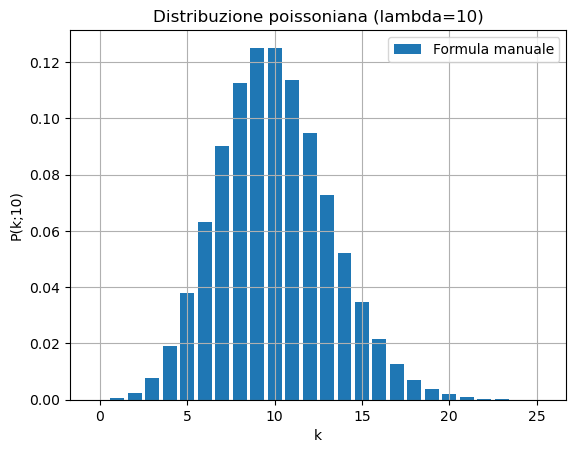
\includegraphics[width=\textwidth]{Immagini/poisson y=10.png} 
        \caption{}
    \end{subfigure}
    \hfill 
    \begin{subfigure}[b]{0.45\textwidth}
        \centering
        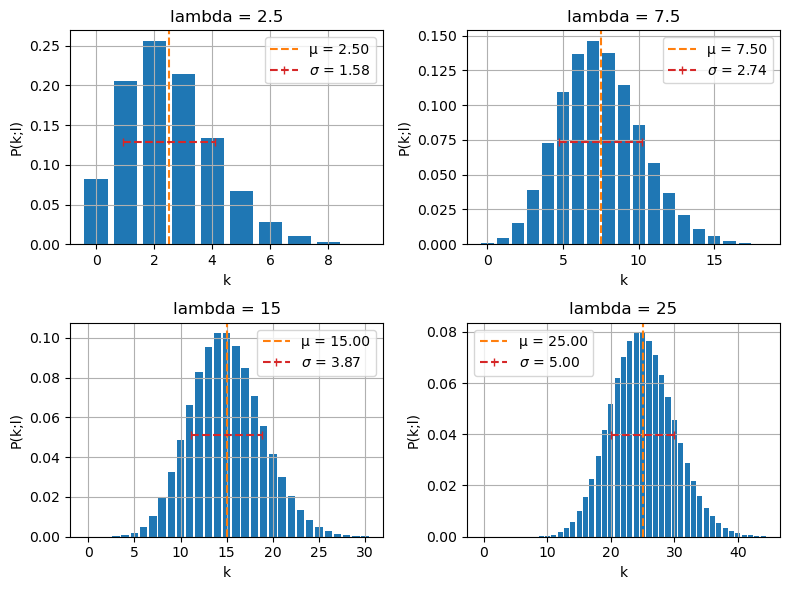
\includegraphics[width=\textwidth]{Immagini/poisson diversi y.png}
        \caption{}
    \end{subfigure}
    
    \vspace{1cm} 
    
    \begin{subfigure}[b]{0.8\textwidth}
        \centering
        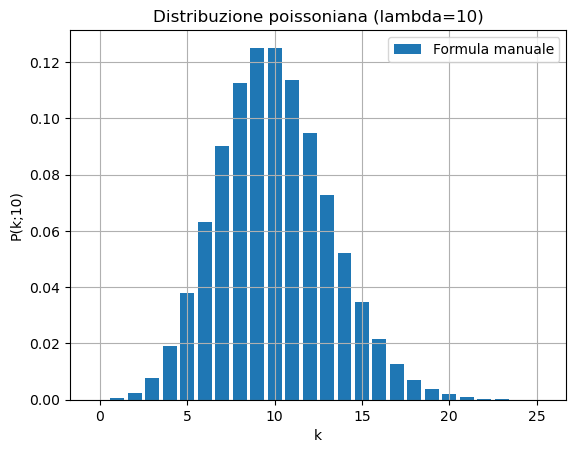
\includegraphics[width=\textwidth]{Immagini/poisson y=10.png}
        \caption{}
    \end{subfigure}
    \hfill 
    \begin{subfigure}[b]{0.45\textwidth}
        \centering
        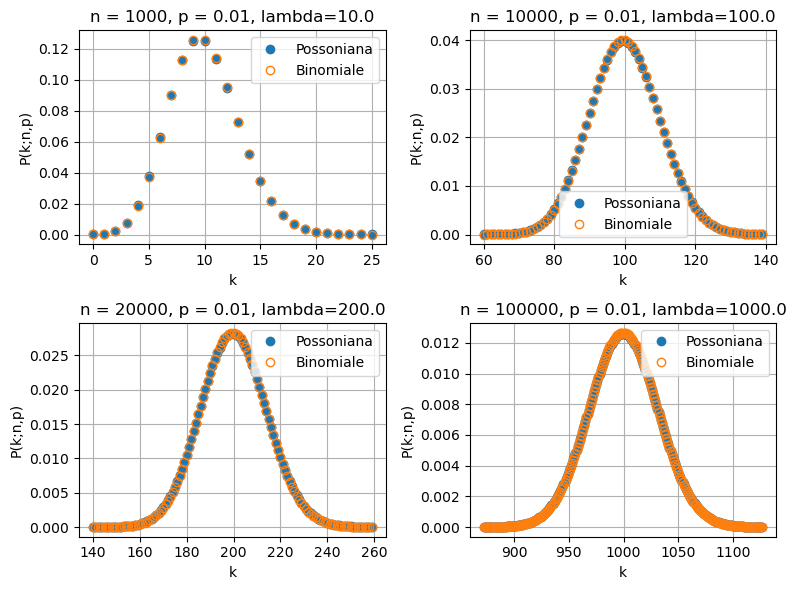
\includegraphics[width=\textwidth]{Immagini/confronto binom poisson e aprox a infinito.png}
        \caption{}
    \end{subfigure}
    
    \caption{Distribuzioni di Poisson e nel limite e confronto binomiale/poissoniana}
\end{figure}


\subsection{Rappresentazione grafica dei dati (Istogrammi)}

Consideriamo un esperimento volto a misurare una grandezza fisica continua $X$. Il modello teorico che descrive il fenomeno fornisce una densità di probabilità $P(x)$, tale che:

\begin{equation}
\int_{-\infty}^{+\infty} P(x) \, dx = 1
\end{equation}

Si effettuano $N$ misure indipendenti di $X$, ottenendo un campione di dati $\{x_1, x_2, \dots, x_N \}$. Questi dati vengono rappresentati graficamente tramite un istogramma, suddividendo l'asse delle $x$ in intervalli adiacenti chiamati \textit{bin}.
Considerando un generico bin $i$, definito nell'intervallo $[x_i, x_{i+1}]$, il numero di eventi $M_i$ che cadono in tale intervallo è una variabile aleatoria discreta. La probabilità teorica che una singola misura cada nel bin $i$ è data da:

\begin{equation}
P_i = \int_{x_i}^{x_{i+1}} P(x) \, dx \approx P\left(x_i + \frac{\Delta x}{2}\right) \Delta x
\end{equation}
dove si assume che il bin sia sufficientemente stretto ($\Delta x$) da poter considerare $P(x)$ costante al suo interno, approssimandola con il valore nel punto centrale.

La variabile $M_i$ segue una statistica binomiale, poiché per ogni singola misura si verificano due sole possibilità: il conteggio cade nel bin $i$ (successo) oppure no (insuccesso).
Il valore di aspettazione di $M_i$ è $\langle M_i \rangle = N P_i$, mentre la varianza è $V_i = N P_i (1-P_i)$.
Al limite, per $P_i$ piccolo e $N$ grande, la distribuzione degli eventi tende a una Poissoniana. In questo caso, il valore di aspettazione è semplicemente $M_i$ e la deviazione standard è stimata come $\sigma = \sqrt{M_i}$.
Per questo motivo, quando si rappresenta un istogramma, si aggiungono spesso delle barre di errore verticali che rappresentano la deviazione standard $\sqrt{M_i}$.

È fondamentale sottolineare che l'istogramma non è una distribuzione di probabilità continua, ma una stima basata su un numero finito di eventi. Il fatto che la fluttuazione dei conteggi nei bin segua una statistica binomiale (o approssimativamente Poissoniana) riguarda il processo di misura e campionamento, ed è concettualmente distinto dalla forma funzionale $P(x)$ del processo fisico sottostante.

Se $P_i$ fosse nota a priori, per un confronto visivo con l'istogramma si potrebbe graficare la curva teorica sopra i dati. Tuttavia, è necessario scalare opportunamente la funzione, poiché l'istogramma riporta il numero di conteggi $M_i \approx P(x_{\text{centro}}) \Delta x N$.

\begin{nota}
\begin{enumerate}
    \item L'approssimazione binomiale e Poissoniana per i conteggi nei bin è valida propriamente se $N$ non è fissato a priori, ma è esso stesso una variabile aleatoria (ad esempio, se si acquisiscono conteggi per un intervallo di tempo fissato, il numero totale $N$ di eventi varierà da esperimento a esperimento). Se invece $N$ è fissato rigorosamente (si decide di acquisire esattamente un certo numero di eventi totali), la distribuzione congiunta dei conteggi nei vari bin segue una distribuzione \textbf{multinomiale}.
    \item Qualunque confronto tra l'istogramma e la curva teorica $P(x)$ basato sulla sovrapposizione grafica è puramente qualitativo. Esistono metodi statistici quantitativi (test di bontà del fit) per valutare la compatibilità, che verranno trattati in seguito.
\end{enumerate}
\end{nota}

\begin{example}
    Se abbiamo una generazione causale di numeri che segue una distribuzione uniforme: $U(0,1)$, allora avrò:
    \[
    P_i=\int_{x_i}^{x_{i+1}} 1 \, dx = \Delta x
    \]
    poichè la distribuzione è fatta così
    \[
    U(0,1)= 
    \begin{cases}
    \text{cost.} &  \text{se x $\in$ (0,1)} \\
    0 & \text{altrimenti}
    \end{cases}
    \]
    poichè deve essere normalizzata deve essere $cost.=1$
\end{example}


\lezione{La Distribuzione Normale (Gaussiana)}{02 Marzo 2026}

\subsection{Definizione e Proprietà Fondamentali}
\ripasso{Distribuzione Normale}

Data una variabile casuale $x$, la funzione di densità di probabilità normale è definita come:
\[
f(x) = N(\mu,\sigma^2) = \frac{1}{\sqrt{2\pi}\sigma}e^{-\frac{(x-\mu)^2}{2\sigma^2}}
\]

\begin{center}
    \begin{tikzpicture}[scale=1.5]
    
    % Corpo del papero
    \filldraw[yellow!70!orange, thick] (0,0) ellipse (1.5 and 1);
    
    % Testa
    \filldraw[yellow!70!orange, thick] (1.8,0.7) circle (0.7);
    
    % Occhio
    \filldraw[white] (2,0.9) circle (0.15);
    \filldraw[black] (2,0.9) circle (0.05);
    
    % Becco
    \filldraw[orange!80!red] (2.3,0.7) -- (2.8,0.7) -- (2.3,0.4) -- cycle;
    
    % Ali stilizzate (o dettagli)
    \draw[thick, yellow!60!brown] 
        (-0.5,0.3) to[out=30, in=210] (0.5,0.8)
        (-0.6,0) to[out=20, in=200] (0.6,0.5);
    
    % Zampe
    \draw[red!80!black, thick] 
        (-0.3,-1) -- (-0.3,-1.3) -- (-0.5,-1.4)
        (0.3,-1) -- (0.3,-1.3) -- (0.5,-1.4);
    
    % Coda
    \draw[thick, yellow!60!brown] (-1.4,0.2) to[out=120, in=240] (-1.6,0.5);
    
    % Fumetto
    \draw[white, fill=white] (2.5,1.5) -- (3,1.8) -- (2.8,1.3) -- cycle;
    \node at (3.3,1.8) {\footnotesize \textbf{Quarck!}}; % Quark/Quack pun
    
    \end{tikzpicture}
\end{center}

Questa funzione rispetta le proprietà fondamentali delle distribuzioni di probabilità:
\begin{itemize}
    \item \textbf{Normalizzazione:}
    \[
        \frac{1}{\sqrt{2\pi}\sigma} \int_{-\infty}^{+\infty} e^{-\frac{(x-\mu)^2}{2\sigma^2}} \, dx = 1
    \]
    \item \textbf{Valore di aspettazione:} corrisponde a $\mu$
    \[
        E[x] = \frac{1}{\sqrt{2\pi}\sigma} \int_{-\infty}^{+\infty} x \, e^{-\frac{(x-\mu)^2}{2\sigma^2}} \, dx = \mu
    \]
    \item \textbf{Varianza:} vale $\sigma^2$
    \[
        \text{Var}(x) = \frac{1}{\sqrt{2\pi}\sigma} \int_{-\infty}^{+\infty} (x - \mu)^2 \, e^{-\frac{(x-\mu)^2}{2\sigma^2}} \, dx = \sigma^2
    \]
\end{itemize}

Per centrare la distribuzione in $0$, si applica la sostituzione $y=x-\mu$ (con $dy=dx$), ottenendo:
\[
f(y; 0, \sigma^2)=\frac{1}{\sqrt{2\pi}\sigma}e^{-\frac{y^2}{2\sigma^2}}
\]
Per standardizzarla (centrata in $0$ e con varianza $\sigma^2=1$), si pone $y=\frac{x-\mu}{\sigma}$ (con $dy=\frac{dx}{\sigma}$), ottenendo la \textbf{distribuzione normale standard}:
\[
f(y; 0, 1)=\frac{1}{\sqrt{2\pi}}e^{-\frac{y^2}{2}}
\]

È interessante notare che, per la distribuzione standard, la funzione di ripartizione $F(x)$ gode della proprietà di simmetria:
\[
F(-x) = 1 - F(x)
\]
Se vogliamo calcolare la probabilità che $x$ cada in un intervallo $[a,b]$:
\[
P(a\leq x\leq b) = P(x \leq b) - P(x \leq a) = F(b) - F(a)
\]
Passando alla variabile standardizzata $z = \frac{x-\mu}{\sigma}$:
\[
P\left(\frac{a- \mu}{\sigma} \leq \frac{x- \mu}{\sigma} \leq \frac{b- \mu}{\sigma}\right) = F\left(\frac{b- \mu}{\sigma}\right) - F\left(\frac{a- \mu}{\sigma}\right)
\]
Scegliendo intervalli simmetrici rispetto alla media, ovvero $a= \mu - n\sigma$ e $b= \mu + n\sigma$:
\[
P(\mu - n\sigma \leq x \leq \mu + n\sigma) = F(n) - F(-n) = F(n) - [1 - F(n)] = 2F(n) - 1
\]
Si può concludere che è molto improbabile (o "anormale") trovare valori molto distanti dalla media. Ad esempio, per $n=3$, la probabilità di cadere all'interno dell'intervallo è circa $0.997$ (o $99.7\%$).

Graficamente:
\begin{itemize}
    \item Il picco della campana si trova in $x=\mu$.
    \item L'altezza del picco è $f(\mu) = \frac{1}{\sqrt{2\pi}\sigma} \approx \frac{0.399}{\sigma}$.
    \item Il valore a metà altezza (FWHM) corrisponde a una larghezza di $2\sqrt{2 \ln(2)}\sigma \approx 2.355\sigma$.
\end{itemize}    

\subsubsection*{Esempio di distribuzione di Gauss}
Consideriamo un esempio basato sulla distribuzione binomiale per modellare gli errori di misura.
Assumiamo le seguenti ipotesi:
\begin{itemize}
    \item L'errore di misura è definito come $u = x - a$ (dove $x$ è il valore misurato e $a$ è il valore vero).
    \item L'errore totale è la somma di $n$ contributi elementari (errori piccoli), ciascuno di valore $\varepsilon$.
\end{itemize}
Ogni contributo $\varepsilon$ può essere positivo o negativo con probabilità $50/50$ (analogia con il cammino casuale). Se indichiamo con $k$ il numero di contributi positivi, allora $(n-k)$ saranno i contributi negativi. L'errore totale sarà:
\[
u_k = k\varepsilon - (n-k)\varepsilon = (2k - n)\varepsilon
\]
Il valore di aspettazione è $E[u_k] = 0$. Per il teorema del limite centrale, quando $n \rightarrow \infty$, la distribuzione di questi errori tende a una gaussiana centrata in 0.

\subsubsection*{Dimostrazione Euristica}
Vogliamo giustificare euristicamente perché la distribuzione degli errori accidentali è gaussiana.
Come visto sopra, se abbiamo $k$ deviazioni positive su $n$ totali, l'errore e la sua probabilità (data dalla binomiale) sono:
\[
u_k=(2k-n) \varepsilon \hspace{1cm} P(k)=\frac{n!}{k!(n-k)!} \left(\frac{1}{2}\right)^n
\]
Considerando due valori successivi $k$ e $k+1$, possiamo definire un valore medio per l'errore e l'incremento:
\[
u^M \approx (2k-n+1)\varepsilon \hspace{1cm} \Delta u = u_{k+1} - u_k = 2 \varepsilon
\]
Per $\Delta u \rightarrow 0$ (cioè $\varepsilon$ molto piccolo e $n$ grande), possiamo passare al continuo. La \textbf{densità di probabilità} $y(u)$ può essere approssimata considerando la variazione di probabilità.
Definiamo la variazione relativa della probabilità:
\[
\frac{\Delta P}{P} \approx \frac{P(k+1) - P(k)}{P(k)}
\]
Svolgendo i calcoli con i fattoriali, si trova che questa variazione è legata all'errore $u$ da una relazione del tipo:
\[
\frac{dy}{y} = -\frac{u}{\sigma^2} \, du
\]
dove $\sigma^2 \propto n\varepsilon^2$. Questa è un'equazione differenziale la cui soluzione è:
\[
\ln y = -\frac{u^2}{2\sigma^2} + C \implies y(u) = A e^{-\frac{u^2}{2\sigma^2}}
\]
Imponendo la normalizzazione, si ottiene la forma gaussiana:
\[
y(u)=\frac{1}{\sqrt{2\pi} \sigma}e^{-\frac{u^2}{2 \sigma^2}}
\]

\textbf{Breve riassunto}
\begin{itemize}[itemsep=0.3em]
    \item Definizione di variabile casuale discreta e continua.
    \item Definizione di funzione di ripartizione $F_x(x)$.
    \item Definizione di funzione di distribuzione (densità di probabilità).
    \item Valori di aspettazione come indici di posizione (media) e dispersione (varianza).
    \item Esempi di funzioni di distribuzione (Binomiale, Poisson, Gaussiana).
\end{itemize}

\subsection{Definizione di distribuzione normale}

La funzione di distribuzione di Gauss, o distribuzione normale, è descritta dalla seguente funzione (Gauss la utilizzò per descrivere gli errori di misura, notando che molti fenomeni naturali tendono a distribuirsi attorno a un valore medio):

\begin{equation}
P(x; \mu , \sigma ) = N(\mu,\sigma^2) = \frac{1}{\sqrt{2\pi}\sigma}e^{-\frac{(x-\mu)^2}{2\sigma^2}}
\end{equation}

dove il simbolo $N$ indica che si tratta di una distribuzione normale.
Graficamente ha la forma di una campana simmetrica centrata in $x = \mu$. La larghezza della curva è determinata dal parametro $\sigma$, che rappresenta la deviazione standard della distribuzione (mentre $\mu$ rappresenta il valore atteso): se $\sigma$ è grande, la distribuzione risulta molto allargata; viceversa, se $\sigma$ è piccolo, la distribuzione è stretta.
Variare $\mu$ equivale a traslare la distribuzione lungo l'asse $x$ senza alterarne la forma, mentre variare $\sigma$ modifica l'ampiezza della curva senza cambiarne il centro.

Nel caso specifico in cui $\mu = 0$ e $\sigma^2 = 1$, si parla di \textbf{distribuzione normale standard}, indicata con $N(0,1)$:

\begin{equation}
N(0,1) = \frac{1}{\sqrt{2 \pi}} e^{-\frac{x^2}{2}}
\end{equation}

È importante notare che, attraverso il cambiamento di variabile $z = \frac{x-\mu}{\sigma}$, una qualsiasi gaussiana può essere ridotta alla forma normale standard in funzione di $z$:

\begin{equation}
P_z(z) = \frac{1}{\sqrt{2 \pi}} e^{-\frac{z^2}{2}}
\end{equation}

Da un punto di vista pratico, questa proprietà è molto utile per i calcoli: se $x$ è una variabile con distribuzione $N(\mu, \sigma^2)$ e $z$ ha una densità di probabilità $N(0,1)$, possiamo passare da $z$ a $x$ utilizzando la formula di trasformazione:

\begin{equation}
z = \frac{x-\mu}{\sigma}
\end{equation}

Utilizzando la formula inversa, possiamo ricavare $x$ noto $z$:

\begin{equation}
z\sigma = x - \mu \implies x = \mu + z\sigma
\end{equation}

\begin{nota}[Note sul Cambio di Variabile]
Quando si effettua un cambio di variabile, la condizione di normalizzazione della probabilità deve essere preservata:
\[
\int_{-\infty}^{+\infty} P_z(z) \, dz = \int_{-\infty}^{+\infty} P_x(x) \, dx = 1
\]
La relazione tra le densità di probabilità è data da:
\[
P_z(z) = P_x [x(z)] \left| \frac{dx}{dz} \right|
\]
Dato che $x(z) = \mu + z\sigma$, la derivata risulta $\frac{dx}{dz} = \sigma$. Sostituendo nella formula precedente si ottiene:
\[
P_z(z) = \frac{1}{\sqrt{2 \pi \sigma^2}} e^{-\frac{(x-\mu)^2}{2\sigma^2}} \cdot \sigma = \frac{1}{\sqrt{2 \pi}} e^{-\frac{z^2}{2}}
\]
che conferma il passaggio alla forma standard.
\end{nota}

\subsection{Calcolo del Valore di Aspettazione e della Varianza}

Come per le altre distribuzioni, possiamo utilizzare la funzione generatrice dei momenti per calcolare il valore di aspettazione e la varianza. A differenza delle distribuzioni discrete viste in precedenza, notiamo che in questo caso $x$ è una variabile continua.

Partiamo dalla funzione generatrice dei momenti centrali:
\begin{equation}
\bar{M}_x(t) = E[e^{t(x-\mu)}] = \int_{-\infty}^{+\infty} e^{t(x-\mu)} P(x) \, dx
\end{equation}

Sostituendo l'espressione di $P(x)$:

\begin{equation}
\bar{M}_x(t) = \frac{1}{\sqrt{2\pi \sigma^2}} \int_{-\infty}^{+\infty} e^{t(x-\mu)} e^{-\frac{(x-\mu)^2}{2\sigma^2}} \, dx = \frac{1}{\sqrt{2\pi \sigma^2}} \int_{-\infty}^{+\infty} \exp \left[ t(x-\mu) - \frac{(x-\mu)^2}{2\sigma^2} \right] \, dx
\end{equation}

Per risolvere l'integrale, riscriviamo l'esponente completando il quadrato:

\begin{equation}
t(x-\mu) - \frac{(x-\mu)^2}{2\sigma^2} = - \frac{\left[ (x-\mu) - \sigma^2 t \right]^2}{2\sigma^2} + \frac{\sigma^2 t^2}{2}
\end{equation}

Infatti, svolgendo il quadrato al numeratore si verifica l'uguaglianza:
\begin{equation}
-\frac{\left[ (x-\mu) - \sigma^2 t \right]^2}{2\sigma^2} = -\frac{(x-\mu)^2 - 2 \sigma^2 t (x-\mu) + \sigma^4 t^2}{2\sigma^2} = -\frac{(x-\mu)^2}{2\sigma^2} + t(x-\mu) - \frac{\sigma^2 t^2}{2}
\end{equation}
Quindi, il termine aggiuntivo $-\frac{\sigma^2 t^2}{2}$ viene compensato aggiungendo $+\frac{\sigma^2 t^2}{2}$. L'integrale diventa:

\begin{equation}
\begin{aligned}
\bar{M}_x(t) &= \frac{1}{\sqrt{2\pi \sigma^2}} \int_{-\infty}^{+\infty}  \exp\left[ -\frac{\left[ (x-\mu) - \sigma^2 t \right]^2}{2\sigma^2} + \frac{\sigma^2 t^2}{2} \right] \, dx \\
&= e^{\frac{\sigma^2 t^2}{2}} \underbrace{\frac{1}{\sqrt{2\pi \sigma^2}} \int_{-\infty}^{+\infty} e^{-\frac{\left[ (x-\mu) - \sigma^2 t \right]^2}{2\sigma^2}} \, dx}_{=1}
\end{aligned}
\end{equation}

L'integrale evidenziato vale 1 poiché rappresenta l'area totale di una gaussiana con media $\mu' = \mu + \sigma^2 t$ e varianza $\sigma^2$. Pertanto otteniamo:
\begin{equation} \boxed{
\bar{M}_x(t) = e^{\frac{\sigma^2 t^2}{2}}}
\end{equation}

Da questo risultato possiamo ricavare la funzione generatrice dei momenti rispetto all'origine $M_x(t)$ usando la relazione $M_x(t) = E[e^{tx}] = E[e^{t(x-\mu)} e^{\mu t}] = e^{\mu t} \bar{M}_x(t)$:

\begin{equation}
M_x(t) = e^{\mu t} \bar{M}_x(t)
\end{equation}

Nel caso particolare di una gaussiana centrata in zero ($\mu=0$) con varianza unitaria ($\sigma^2=1$), si ha $\bar{M}_x(t)=M_x(t)$.
Per una gaussiana generale si ottiene quindi:
\begin{equation} \boxed{
M_x(t) = \exp\left(\mu t + \frac{\sigma^2 t^2}{2}\right)}
\end{equation}

Ora possiamo calcolare il valore di aspettazione derivando $M_x(t)$:

\begin{equation}
\frac{d M_x}{dt} = \frac{d}{dt} \left[ \exp\left( \mu t + \frac{\sigma^2 t^2}{2} \right) \right] = \left( \mu + \sigma^2 t \right) e^{\mu t + \frac{\sigma^2 t^2}{2}}
\end{equation}
Valutando la derivata in $t = 0$:
\begin{equation}
\frac{d M_x}{dt} \bigg\rvert_{t=0} = \mu = E[x] 
\end{equation}

Per calcolare la varianza è conveniente utilizzare la derivata seconda della funzione generatrice dei momenti centrali (o continuare a derivare $M_x$):
\begin{equation}
\frac{d \bar{M}_x}{dt} \bigg\rvert_{t=0} = 0 \quad \text{e} \quad \frac{d^2 \bar{M}_x}{dt^2} \bigg\rvert_{t=0} = \sigma^2
\end{equation}
Se calcoliamo la derivata seconda di $M_x(t)$:
\begin{equation}
\frac{d^2 M_x}{dt^2} = \left[ \sigma^2 + (\mu + \sigma^2 t)^2 \right] e^{\mu t + \frac{\sigma^2 t^2}{2}}
\end{equation}
Tuttavia, usando la funzione generatrice dei momenti centrali $\bar{M}_x(t) = e^{\frac{\sigma^2 t^2}{2}}$, la derivata prima è $\sigma^2 t e^{\frac{\sigma^2 t^2}{2}}$ e la seconda:
\begin{equation}
\frac{d^2 \bar{M}_x}{dt^2} = (\sigma^2 + \sigma^4 t^2) e^{\frac{\sigma^2 t^2}{2}}
\end{equation}
Per $t=0$, l'esponenziale diventa 1, quindi:
\begin{equation}
\frac{d^2 \bar{M}_x}{dt^2} \bigg\rvert_{t=0} = \sigma^2 = \text{Var}(x)
\end{equation}

Procedendo con le derivate successive si può osservare che tutti i momenti centrali di ordine dispari sono nulli ($\mu_3 = 0$, ecc.), il che conferma la simmetria della distribuzione.

In particolare, per la normale standard $N(0,1)$, si ha:
\begin{equation}
M_x(t) = \bar{M}_x(t) = e^{\frac{t^2}{2}}
\end{equation}

\ripasso{Confronto istogramma/gaussiana}
Date 100 misure che cadono in $k$ intervalli di valore centrale $x^k$ e larghezza $\Delta x$, ci chiediamo quale sia la funzione di distribuzione che mi definisca la probabilità che un certo dato cada in un
certo intervallo (successo), questa è la \textbf{funzione di distribuzione binomiale}:

Sapendo che la probabilità per un intervallo $k$ è: $P_k= \binom{n}{l}p^l(1-p)^{n-l}$, dove $p$ è la probabilità di successo e $l$ il numero di successi, so che $E[l]=np$ e  $\sigma^2= np(1-p)$.

Considerando ora una distribuzione di tipo Gaussiano la funzione che la descrive é la classica e la probabilità che un certo valore cada in un intervallo è:
\[
P_k=\int_{x_i -\frac{\Delta x}{2}}^{x_i + \frac{\Delta x}{2}} f(x, \hat{\mu}, \sigma^2) dx \simeq f(\bar{x}_k) \Delta x. 
\]
da cui ottengo il numero di eventi atteso all'interno dell'intervallo $n_k$ e per ogni intervallo ho un certo $\sigma$, per ognuno di questi intervalli posso fare un confronto per verificare la compatibilità
\begin{equation*}
\left| {n_k}^s-{n_k}^m \right| \leq 3 \sigma_k
\end{equation*}
dove $m$ sta per eventi misurati ed $s$ per eventi attesi, avremo quindi un grafico con un valore atteso di eventi con barra di errore di larghezza $\sigma$, dunque in un grafico mi aspetto che:
\begin{itemize}
\item il 68\% deve toccare con le barre di errore il valore di aspettazione
\item il 27\% si trova a 2 $\sigma$
\item il 5\% si trova a 3 $\sigma$
\end{itemize}
La deviazione standard della binomiale è circa $\sqrt{n_k^m}$ se $n_{tot}>>>n_k^c$, che in realtà è un approssimazione che va bene quando $n_k^c > 5$

\subsection{Variabili Aleatorie e Combinazioni Lineari}

Si può dimostrare un importante teorema: una combinazione lineare di variabili casuali normali e statisticamente indipendenti è anch'essa distribuita secondo una legge normale.
Per la dimostrazione utilizziamo la funzione generatrice dei momenti. Supponiamo di avere $X_1, X_2, \dots, X_M$ variabili aleatorie indipendenti, ognuna descritta da una gaussiana $N_i(\mu_i, \sigma_i^2)$. Una loro combinazione lineare può essere scritta come:

\begin{equation}
S = \sum_{i=1}^{k} a_i x_i
\end{equation}
dove $a_i$ sono i coefficienti scalari.
Definendo $y_i= a_i x_i$, vogliamo dimostrare che $S$ ha una densità di probabilità gaussiana.
La funzione generatrice di momenti per ogni $x_i$ è:

\begin{equation}
M_{x_i}(t) = \exp \left( \mu_i t + \frac{1}{2} \sigma_i^2 t^2 \right)
\end{equation}

Sappiamo che per la somma di variabili indipendenti $z = \sum x_i$ vale la proprietà:
\begin{equation}
M_z(t) = \prod_{i} M_{x_i}(t)  
\end{equation}
Inoltre, per il prodotto di una variabile per una costante $y = ax$, vale:
\begin{equation}
M_y(t) = E[e^{t y}] = E[e^{tax}] = M_x(at) 
\end{equation}

Applicando queste proprietà alla nostra somma $S = \sum_{i} y_i$ (dove $y_i = a_i x_i$), otteniamo:
\begin{equation}
M_s(t) = \prod_{i} M_{y_i}(t) = \prod_{i} M_{x_i}(a_i t)
\end{equation}

Sostituendo la forma funzionale della gaussiana:
\begin{equation}
M_s(t) = \prod_{i} \left[ \exp \left( \mu_i (a_i t) + \frac{1}{2} \sigma_i^2 (a_i t)^2 \right) \right]
\end{equation}

Utilizzando la proprietà degli esponenziali per cui il prodotto di esponenziali è l'esponenziale della somma degli esponenti:
\begin{equation}
M_s(t) = \exp \left[ \left(\sum_{i} \mu_i a_i\right) t + \frac{1}{2} \left( \sum_{i} \sigma_i^2 a_i^2 \right) t^2 \right]
\end{equation}

Il risultato mostra che la funzione generatrice di $S$ ha la stessa forma funzionale di una gaussiana. Dunque, una variabile dipendente linearmente da altre variabili normali indipendenti avrà anch'essa distribuzione normale, con parametri:

\begin{equation}
\mu_s = \sum_{i} \mu_i a_i
\end{equation}

\begin{equation}
\sigma_s^2 = \sum_{i} \sigma_i^2 a_i^2
\end{equation}

È importante notare che la gaussiana è l'unica distribuzione a varianza finita che gode di questa proprietà (stabilità rispetto alle combinazioni lineari).
Ad esempio, per la distribuzione di Poisson, la somma di variabili indipendenti $y = \sum x_i$ è ancora una Poissoniana, ma la moltiplicazione per una costante non preserva la distribuzione. Se $y=ax$, la funzione generatrice diventa:
\begin{equation}
M_y(t) = M_x(at) = \exp [\lambda (e^{at} - 1)]
\end{equation}
Questa espressione corrisponde a una Poissoniana solo se $a=1$.
Il motivo per cui il "trucco" funziona per la gaussiana risiede nel fatto che l'esponente della sua $M_x(t)$ è un polinomio di secondo grado in $t$: la sostituzione $t \to at$ mantiene il polinomio di secondo grado, preservando così la forma della distribuzione.


\lezione{Teorema del Limite Centrale}{05 Marzo 2026}

Il Teorema del Limite Centrale è un risultato fondamentale della statistica. Esso giustifica l'utilizzo della distribuzione gaussiana (o normale) per descrivere i risultati di misurazioni fisiche, specialmente quando queste sono affette da molteplici cause di errore indipendenti.

\begin{theorem*}
    Consideriamo un insieme di $n$ variabili aleatorie \textbf{indipendenti} $\{x_1, \dots, x_n\}$.
    Assumiamo che ciascuna variabile $x_i$ abbia una densità di probabilità $P_i(x)$ e che il suo valore atteso (media) $E[x_i]=\mu_i$ e la sua varianza $\text{var}(x_i)=\sigma_i^2$ \textbf{esistano e siano finiti}.

    Definiamo la variabile aleatoria $S$ come la somma delle $n$ variabili:
    \[
    S = \sum_{i=1}^{n} x_i
    \]
    
    Il valore atteso e la varianza di $S$ sono dati da (proprietà dimostrabili per variabili indipendenti):
    \[
    E[S] = \sum_{i=1}^{n} \mu_i \hspace{2cm} \text{var}(S) = \sum_{i=1}^{n} \sigma_i^2
    \]
    
    Il teorema afferma che, per $n \to \infty$, la distribuzione di $S$ tende a una distribuzione normale:
    \[
    S \overset{n \to \infty}{\sim} \mathcal{N} \left(\sum_{i=1}^{n} \mu_i, \sum_{i=1}^{n} \sigma_i^2 \right)
    \]
\end{theorem*}

Nella pratica, l'approssimazione è spesso già accettabile per $n \ge 10$.

È possibile riformulare il teorema utilizzando la variabile standardizzata. Applicando la trasformazione $z = \frac{\text{valore} - \text{media}}{\text{dev.std}}$, otteniamo:
\[
Z_n = \frac{S - \sum_{i=1}^{n} \mu_i}{\sqrt{\sum_{i=1}^{n} \sigma_i^2}} \overset{n \to \infty}{\sim} \mathcal{N}(0,1)
\]

\subsection{Caso Particolare: Variabili I.I.D.}
Un caso molto comune è quello in cui le variabili $x_i$ sono \textbf{indipendenti e identicamente distribuite} (I.I.D.). In questo scenario, le ipotesi si semplificano:
\begin{itemize}
    \item Tutte le variabili hanno la stessa distribuzione: $P_i(x) = P(x)$;
    \item Stessa media: $\mu_i = \mu$;
    \item Stessa deviazione standard: $\sigma_i = \sigma$.
\end{itemize}

Di conseguenza, i parametri della somma $S$ diventano:
\begin{itemize}
    \item $E[S] = \sum_{i=1}^n \mu = n\mu$
    \item $\text{var}(S) = \sum_{i=1}^n \sigma^2 = n\sigma^2$
\end{itemize}

La variabile standardizzata assume quindi la forma:
\begin{equation}
Z_n = \frac{S - n\mu}{\sqrt{n\sigma^2}} = \frac{S - n\mu}{\sigma\sqrt{n}}
\end{equation}

Dividendo numeratore e denominatore per $n$, possiamo esprimere il risultato in termini della \textbf{media campionaria} $\bar{x} = \frac{S}{n} = \frac{\sum x_i}{n}$:
\begin{equation}
Z_n = \frac{\frac{S - n\mu}{n}}{\frac{\sigma\sqrt{n}}{n}} = \frac{\frac{S}{n} - \mu}{\frac{\sigma}{\sqrt{n}}} = \frac{\bar{x} - \mu}{\frac{\sigma}{\sqrt{n}}}
\end{equation}

Questo implica che, per $n \to \infty$:
\begin{equation}
\frac{\bar{x} - \mu}{\sigma / \sqrt{n}} \sim \mathcal{N}(0, 1)
\end{equation}
Ovvero, la media campionaria $\bar{x}$ tende a distribuirsi secondo una normale con media $\mu$ e varianza ridotta:
\[
\bar{x} \overset{n\to\infty}{\sim} \mathcal{N}\left(\mu, \frac{\sigma^2}{n}\right)
\]

Per tornare alla variabile non standardizzata, invertiamo la relazione:
\[
z = \frac{\bar{x}-\mu}{\sigma/\sqrt{n}} \implies \bar{x} = \mu + z \frac{\sigma}{\sqrt{n}}
\]

\subsection{Dimostrazione (tramite Funzione Generatrice dei Momenti)}
Dimostriamo il teorema nel caso I.I.D., ovvero proviamo che:
\[
\lim_{n \to \infty} \frac{S - n\mu}{\sigma \sqrt{n}} \sim \mathcal{N}(0,1)
\]

Per semplificare i calcoli, partiamo dalle variabili standardizzate delle singole $x_i$. Definiamo:
\[
y_i = \frac{x_i - \mu}{\sigma}
\]
Analizziamo le proprietà di $y_i$:
\begin{itemize}
    \item Valore atteso:
    \[ E[y_i] = E\left[\frac{x_i - \mu}{\sigma}\right] = \frac{1}{\sigma}(E[x_i] - \mu) = \frac{1}{\sigma}(\mu - \mu) = 0 \]
    \item Varianza:
    \[ \text{var}(y_i) = \text{var}\left(\frac{x_i - \mu}{\sigma}\right) = \frac{1}{\sigma^2}\text{var}(x_i) = \frac{\sigma^2}{\sigma^2} = 1 \]
\end{itemize}
(Nota: abbiamo usato le proprietà $E[x-c] = E[x]-c$ e $\text{var}(a(x+c)) = a^2E[{(x+c)}^2]$).

Definiamo ora la variabile somma standardizzata $Z$:
\[
Z = \frac{\sum_{i=1}^{n} y_i}{\sqrt{n}}
\]
Si noti che questa espressione è equivalente a $\frac{S - n\mu}{\sigma\sqrt{n}}$.

Calcoliamo la \textbf{Funzione Generatrice dei Momenti} (MGF) di $Z$, indicata con $M_Z(t)$.
Poiché le $y_i$ sono indipendenti, la MGF della somma è il prodotto delle MGF. Inoltre, ricordando che $M_{aX}(t) = M_X(at)$, otteniamo:
\begin{equation}
M_Z(t) = \prod_{i=1}^n M_{y_i}\left(\frac{t}{\sqrt{n}}\right)
\end{equation}
Essendo le $y_i$ identicamente distribuite, tutte le $M_{y_i}$ sono uguali a una generica $M_y$:
\begin{equation}
M_Z(t) = \left[ M_y\left(\frac{t}{\sqrt{n}}\right) \right]^n
\end{equation}

Sviluppiamo $M_y(k) = E[e^{ky}]$ in serie di Taylor attorno a $k=0$, ponendo $k = t/\sqrt{n}$:
\begin{equation}
e^{ky} = 1 + ky + \frac{k^2 y^2}{2} + \dots \implies e^{ty/\sqrt{n}} = 1 + \frac{ty}{\sqrt{n}} + \frac{t^2 y^2}{2n} + o\left(\frac{1}{n}\right)
\end{equation}
Passando ai valori attesi e ricordando che $E[y]=0$ e $E[y^2] = \text{var}(y) + E[y]^2 = 1$:
\begin{equation}
E\left[ e^{ty/\sqrt{n}} \right] = 1 + \frac{t}{\sqrt{n}}\underbrace{E[y]}_{0} + \frac{t^2}{2n}\underbrace{E[y^2]}_{1} + \dots \simeq 1 + \frac{t^2}{2n}
\end{equation}
Sostituendo questo risultato nella formula di $M_Z(t)$:
\begin{equation}
M_Z(t) \simeq \left( 1 + \frac{t^2}{2n} \right)^n
\end{equation}
Calcoliamo il limite per $n \to \infty$ sfruttando il limite notevole $(1 + \frac{a}{n})^n \to e^a$:
\begin{equation}
\lim_{n \to \infty} M_Z(t) = e^{t^2/2}
\end{equation}
La funzione $e^{t^2/2}$ è esattamente la funzione generatrice dei momenti della normale standard $\mathcal{N}(0,1)$. Per il teorema di unicità delle funzioni generatrici, concludiamo che $Z$ converge in distribuzione alla normale standard.

\subsection{Implicazioni del Teorema nell'Analisi Dati}

Il teorema ha implicazioni cruciali: ci assicura che l'effetto cumulativo di molte piccole perturbazioni indipendenti produce una distribuzione gaussiana, indipendentemente dalla forma della distribuzione di partenza.

Nelle misure fisiche, se ripetiamo una misura $n$ volte, la media aritmetica $\bar{x}$ tende a distribuirsi come $\mathcal{N}(\mu, \sigma^2/n)$. Questo significa che l'incertezza associata alla \textit{media} (deviazione standard della media) è:
\begin{equation}
\sigma_{\bar{x}} = \frac{\sigma}{\sqrt{n}}
\end{equation}
dove $\sigma$ è la deviazione standard della singola misura.

In un esperimento reale, non conosciamo il vero $\sigma$, ma lo stimiamo con la deviazione standard campionaria $s$:
\[
s = \sqrt{\frac{\sum_{i=1}^{n} (x_i-\bar{x})^2}{n-1}}
\]
Il risultato finale di $n$ misure ripetute viene quindi riportato come:
\begin{equation}
\text{Risultato} = \bar{x} \pm \frac{s}{\sqrt{n}}
\end{equation}

Questo intervallo ha un preciso significato probabilistico (intervalli di confidenza):
\begin{itemize}
    \item $\bar{x} \pm 1\sigma_{\bar{x}}$ copre il 68.3\% di probabilità;
    \item $\bar{x} \pm 2\sigma_{\bar{x}}$ copre il 95.5\% di probabilità;
    \item $\bar{x} \pm 3\sigma_{\bar{x}}$ copre il 99.7\% di probabilità.
\end{itemize}

\subsection{Generazione di Numeri Casuali Normali}

Una delle applicazioni informatiche del teorema è la generazione di numeri pseudo-casuali con distribuzione normale a partire da un generatore uniforme (disponibile in tutti i linguaggi di programmazione).

Consideriamo $n$ variabili $\{u_1, \dots, u_n\}$ con distribuzione uniforme in $[0, 1]$.
Per la distribuzione uniforme:
\begin{itemize}
    \item Densità: $P(u) = 1$ per $u \in [0,1]$, $0$ altrimenti.
    \item Media: $E[u] = \int_0^1 u \, du = \frac{1}{2}$.
    \item Secondo momento: $E[u^2] = \int_0^1 u^2 \, du = \frac{1}{3}$.
    \item Varianza: $\text{var}(u) = E[u^2] - E[u]^2 = \frac{1}{3} - \frac{1}{4} = \frac{1}{12}$.
\end{itemize}

Applicando il Teorema del Limite Centrale alla somma, la variabile standardizzata è:
\begin{equation}
Z = \frac{\sum u_i - n E[u]}{\sqrt{n \text{var}(u)}} = \frac{\sum u_i - n/2}{\sqrt{n/12}} \sim \mathcal{N}(0,1)
\end{equation}

Per semplificare il calcolo, si sceglie spesso $n=12$. In questo caso il denominatore diventa $\sqrt{12/12} = 1$ e la formula si riduce a:
\begin{equation}
Z \approx \sum_{i=1}^{12} u_i - 6
\end{equation}
Quindi: si sommano 12 numeri uniformi e si sottrae 6.
\textit{Nota:} Questo metodo è veloce ma approssimato; le "code" della distribuzione (oltre $6\sigma$) sono troncate, poiché la somma di variabili limitate è comunque limitata.

\subsection{La Trasformazione di Box-Muller}
Un metodo matematicamente esatto per generare numeri normali da numeri uniformi è la \textbf{trasformazione di Box-Muller}.

Questo metodo si basa sul cambiamento di variabili per le densità di probabilità. Se abbiamo variabili casuali $x$ legate a variabili $y$ da una trasformazione invertibile, la densità di probabilità congiunta si trasforma secondo:
\begin{equation}
P_y(y_1, \dots, y_n) = P_x(x_1, \dots, x_n) \cdot |J|
\end{equation}
dove $|J|$ è il valore assoluto del determinante Jacobiano della trasformazione inversa (da $y$ a $x$).

Siano $x_1, x_2$ due variabili indipendenti uniformi in $[0, 1]$. Definiamo due nuove variabili $y_1, y_2$:
\begin{align}
y_1 &= \sqrt{-2 \ln x_1} \cos(2\pi x_2) \\
y_2 &= \sqrt{-2 \ln x_1} \sin(2\pi x_2)
\end{align}

Per dimostrare che $y_1$ e $y_2$ sono gaussiane standard indipendenti, invertiamo il sistema per esprimere $x$ in funzione di $y$:
\begin{itemize}
    \item Dal rapporto $y_2/y_1 = \tan(2\pi x_2)$ otteniamo $x_2 = \frac{1}{2\pi} \arctan(y_2/y_1)$.
    \item Dalla somma dei quadrati $y_1^2 + y_2^2 = -2 \ln x_1$ otteniamo $x_1 = \exp\left[-\frac{1}{2}(y_1^2 + y_2^2)\right]$.
\end{itemize}

La densità congiunta delle variabili uniformi è $P_x(x_1, x_2) = 1$ (nel quadrato unitario).
Calcoliamo lo Jacobiano $J = \det \frac{\partial(x_1, x_2)}{\partial(y_1, y_2)}$:
\[
J = \det \begin{pmatrix}
\frac{\partial x_1}{\partial y_1} & \frac{\partial x_1}{\partial y_2} \\
\frac{\partial x_2}{\partial y_1} & \frac{\partial x_2}{\partial y_2}
\end{pmatrix}
\]

Calcolo delle derivate parziali:
\begin{itemize}
    \item $\frac{\partial x_1}{\partial y_1} = -y_1 e^{-\frac{1}{2}(y_1^2+y_2^2)}$
    \item $\frac{\partial x_1}{\partial y_2} = -y_2 e^{-\frac{1}{2}(y_1^2+y_2^2)}$
    \item $\frac{\partial x_2}{\partial y_1} = \frac{1}{2\pi} \frac{1}{1+(y_2/y_1)^2} \left(-\frac{y_2}{y_1^2}\right) = -\frac{1}{2\pi} \frac{y_2}{y_1^2+y_2^2}$
    \item $\frac{\partial x_2}{\partial y_2} = \frac{1}{2\pi} \frac{1}{1+(y_2/y_1)^2} \left(\frac{1}{y_1}\right) = \frac{1}{2\pi} \frac{y_1}{y_1^2+y_2^2}$
\end{itemize}

Calcolando il determinante:
\begin{align*}
J &= \left(-y_1 e^{-\dots}\right)\left(\frac{y_1}{2\pi(y_1^2+y_2^2)}\right) - \left(-y_2 e^{-\dots}\right)\left(-\frac{y_2}{2\pi(y_1^2+y_2^2)}\right) \\
&= -\frac{1}{2\pi} e^{-\frac{1}{2}(y_1^2+y_2^2)} \left( \frac{y_1^2 + y_2^2}{y_1^2 + y_2^2} \right) \\
&= -\frac{1}{2\pi} e^{-\frac{1}{2}(y_1^2+y_2^2)}
\end{align*}

Prendendo il valore assoluto per la densità di probabilità:
\begin{equation}
P_y(y_1, y_2) = 1 \cdot |J| = \frac{1}{2\pi} e^{-\frac{y_1^2 + y_2^2}{2}} = \left(\frac{1}{\sqrt{2\pi}}e^{-y_1^2/2}\right) \cdot \left(\frac{1}{\sqrt{2\pi}}e^{-y_2^2/2}\right)
\end{equation}
Il risultato è il prodotto di due densità normali standard. Quindi $y_1$ e $y_2$ sono variabili $\mathcal{N}(0,1)$ indipendenti.


\begin{lstlisting}[caption={Generazione numeri casuali: Teorema del Limite Centrale e Box-Muller}]
import numpy as np
import matplotlib.pyplot as plt
import scipy.stats as stats

def gaussian_pdf(x, mu=0, sigma=1):
    return (1 / (sigma * np.sqrt(2 * np.pi))) * np.exp(-((x - mu) ** 2) / (2 * sigma ** 2))

# definisco una funzione che dato un array, costruisce l'istogramma e sovrappone una normale standard
def plot_histo_gauss(x, titolo):
    # Parametri richiesti
    # x: array di cui fare l'istogramma
    # titolo: stringa contenente il titolo dell'istogramma

    h, bins, _ = plt.hist(x, range=(-4,4), bins=80, alpha=0.6, label="istogramma")
    delta_x = bins[1] - bins[0]
    centri = (bins[:-1] + bins[1:]) / 2
    # aggiungo una barra di errore seguendo l'approssimazione di Poisson
    plt.errorbar(centri, h, np.sqrt(h), delta_x/2, c='tab:grey', lw=1, fmt='none',label="errore statistico")
    plt.plot(centri, gaussian_pdf(centri)*delta_x*len(x),label='normale standard')
    plt.xlabel("x")
    plt.ylabel("Conteggi")
    plt.title(titolo)
    plt.legend()
    plt.show()

n = 12
m = 10000

# lista dove salvare i numeri generati
lista_gauss =[]
for i in range (m):
    # genero n numeri random tra 0 e 1
    u = np.random.uniform(0, 1, n)

    # li sommo e sottraggo 6
    x = np.sum(u) - 6

    # aggiungo il numero ottenuto alla lista
    lista_gauss.append(x)

# ora faccio un istogramma degli elementi della lista e sovrappongo una normale standard
plot_histo_gauss(lista_gauss, "Generazione da teorema del limite centrale")

# -- Caso della formula di Box-Muller --

# genero m numeri random e ottengo da essi due array x1 e x2 contenenti rispettivamente la prima e la seconda meta' dell'array
x = np.random.uniform(0,1,m)
x1 = x[0:int(m/2)]
x2 = x[int(m/2):m]

print(f"elementi di x {len(x)}, elementi di x1 {len(x1)}, elementi di x2 {len(x2)}")
print(x1[-1],x2[0])

# uso la trasformazione di Box-Muller per ottenere valori distribuiti secondo una normale standard
y1 = np.sqrt(-2*np.log(x1))*np.cos(2*np.pi*x2)
y2 = np.sqrt(-2*np.log(x1))*np.sin(2*np.pi*x2)
y = np.concatenate((y1,y2))
print(f"elementi di y {len(y)}, elementi di y1 {len(y1)}, elementi di y2 {len(y2)}")

plot_histo_gauss(y, "Generazione da Box-Muller")
\end{lstlisting}

\begin{figure}[htbp]
    \centering
    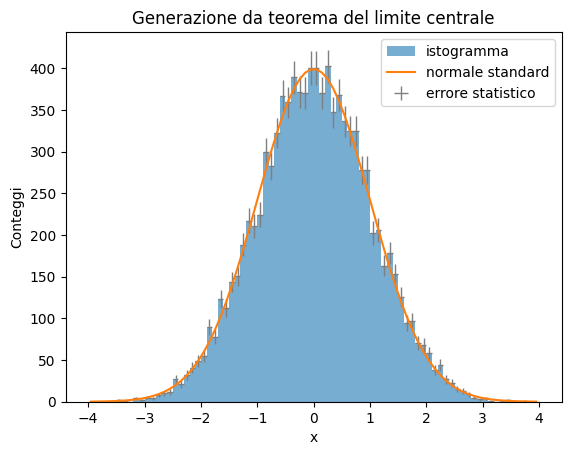
\includegraphics[width=0.48\textwidth]{Immagini/tlc.png}
    \hfill
    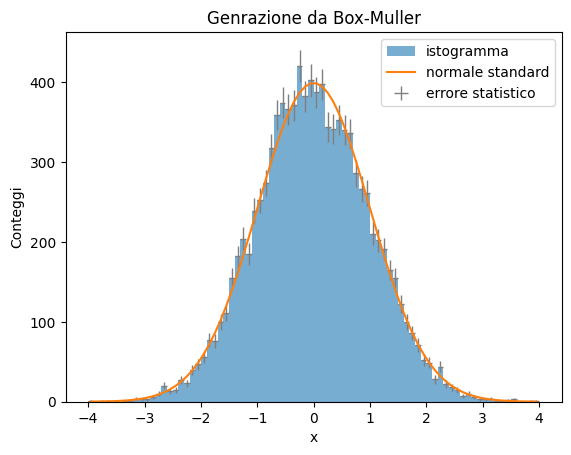
\includegraphics[width=0.48\textwidth]{Immagini/box_muller.png}
    \caption{A sinistra: generazione di una normale standard tramite il Teorema del Limite Centrale. A destra: generazione tramite il metodo di Box-Muller. Entrambi si sovrappongono perfettamente alla curva teorica.}
\end{figure}



\lezione{Distribuzione di Cauchy e Legge dei grandi numeri}{16 Marzo 2026}
\subsection{Distribuzione di Cauchy come rapporto di due normali standard}

Supponiamo che $x_1, x_2$ sono due variabili aleatorie indipendenti normali standard. La loro densità di probabilità congiunta è
\[
P_{x}(x_1, x_2) = \frac{1}{2\pi} \exp\left[ -(x_1^2 + x_2^2)/2 \right]
\]
Quello che ci interessa è studiare la variabile
\[
y_1 = \frac{x_1}{x_2}
\]
Per comodità ci conviene introdurre la variabile $y_2 = x_2$, in modo che la trasformazione diventi:
\[
\begin{cases}
y_1 = x_1 / x_2 \\
y_2 = x_2
\end{cases}
\quad \text{e viceversa} \quad
\begin{cases}
x_1 = y_1 y_2 \\
x_2 = y_2
\end{cases}
\]
Così facendo lo jacobiano della trasformazione è semplicemente
\[
\frac{\partial x_1}{\partial y_1} \frac{\partial x_2}{\partial y_2} - \frac{\partial x_1}{\partial y_2} \frac{\partial x_2}{\partial y_1} = y_2 - y_1 \cdot 0 = y_2
\]
Si ha quindi che
\[
P_y(y_1, y_2) = \frac{1}{2\pi} \exp\left[ -(x_1^2 + x_2^2)/2 \right] |y_2|
\]
Ora scrivo l'esponente in termini di $y_1$ e $y_2$ e ho
\[
- (x_1^2 + x_2^2)/2 = - \frac{(y_1 y_2)^2 + y_2^2}{2} = - \frac{y_2^2 (y_1^2 + 1)}{2}
\]
quindi sostituendo ho
\[
P_y(y_1, y_2) = \frac{|y_2|}{2\pi} \exp\left[ - \frac{y_2^2 (y_1^2 + 1)}{2} \right]
\]
Ora a me serve calcolare $P_y(y_1)$ e per farlo marginalizzo rispetto a $y_2$ cioè integro $P_y(y_1, y_2)$ rispetto a $y_2$
\[
P_y(y_1) = \int_{-\infty}^{+\infty} \frac{|y_2|}{2\pi} \exp\left[ - \frac{y_2^2 (y_1^2 + 1)}{2} \right] dy_2
\]
Essendo la funzione integranda pari in $y_2$ avremo
\[
P_y(y_1) = 2 \int_{0}^{+\infty} \frac{y_2}{2\pi} \exp\left[ - \frac{y_2^2 (y_1^2 + 1)}{2} \right] dy_2
\]
L'integrale che resta è del tipo $\int_{0}^{\infty} x e^{-ax^2} dx$ con $a = \frac{y_1^2 + 1}{2}$. Questo integrale si può risolvere facendo il cambiamento di variabile $u = ax^2 \implies du = 2ax \, dx \implies x \, dx = \frac{1}{2a} du$
\[
\int_{0}^{\infty} x e^{-ax^2} dx = \int_{0}^{\infty} \frac{1}{2a} du \, e^{-u} = \frac{1}{2a} \int_{0}^{\infty} e^{-u} du = \frac{1}{2a} \left[ -e^{-u} \right]_0^\infty = \frac{1}{2a}
\]
Sostituendo si ha quindi che
\[
P_y(y_1) = \frac{1}{\pi} \frac{1}{1 + y_1^2}
\]

La distribuzione di probabilità trovata è la funzione di Cauchy standard, il che dimostra che il rapporto fra due variabili normali segue la distribuzione di Cauchy. \\
Questa distribuzione, anche conosciuta come distribuzione di Breit-Wigner è molto usata in fisica delle particelle in cui la forma di solito è quella che si ottiene con un cambiamento di variabili del tipo $y_1 = \frac{x - x_0}{\Gamma} \implies x = \Gamma y_1 + x_0$
\[
P_X(x) = \frac{1}{\pi} \frac{1}{1 + \left( \frac{x - x_0}{\Gamma} \right)^2} \cdot \left| \frac{dy_1}{dx} \right| = \frac{1}{\pi} \frac{\Gamma^2}{\Gamma^2 + (x - x_0)^2} \cdot \frac{1}{\Gamma} = \frac{1}{\pi} \frac{\Gamma}{\Gamma^2 + (x - x_0)^2}
\]
Di solito questa funzione viene usata perché è una buona approssimazione per descrivere la massa invariante delle risonanze in fisica delle particelle o le intensità delle righe spettrali di emissione o assorbimento negli atomi. Nella formula $x_0$ rappresenta la locazione delle risonanze e $\Gamma$ ha a che fare con la sua larghezza.

La caratteristica di questa distribuzione è che, anche se è simmetrica rispetto a $x_0$ (oppure 0 nella formulazione di Cauchy) si vede che gli integrali
\[
\int_{-\infty}^{0} x P(x) dx \quad \text{e} \quad \int_{0}^{+\infty} x P(x) dx
\]
sono individualmente divergenti, il primo fa $-\infty$ e il secondo $+\infty$ e quindi tecnicamente il valore di aspettazione non è definito. \\
Intuitivamente il problema è che la distribuzione di Cauchy ha code così alte che la media non riesce a stabilizzarsi a un valore preciso. Quando si calcola la media di $n$ eventi, al crescere di $n$, si vede che all'inizio sembra che la media si stabilizzi a zero poi si iniziano a presentare dei salti che spostano la media. Questo perché visto che i valori nelle code della distribuzione non sono tanto rari, ne viene aggiunto uno alla somma con l'effetto di spostare la media. \\
Analogamente la varianza e tutti i momenti di ordine superiore sono divergenti.


\begin{center}
\begin{tikzpicture}[scale=1.2]
    % Asse x
    \draw[->, thick, gray] (-3,0) -- (4,0) node[right, text=black] {$x$};
    % Asse y
    \draw[->, thick, gray] (0,-0.2) -- (0,2.5) node[above, text=black] {$P(x)$};

    % Curva di Cauchy (Coda sinistra)
    \draw[thick, orange!80!black, domain=-3:-0.5, samples=50] plot (\x, {1.5/(1+\x*\x)});
    % Curva di Cauchy (Coda destra - accennata sotto la coda del gatto)
    \draw[dashed, orange!80!black, domain=0.5:3.8, samples=50] plot (\x, {1.5/(1+\x*\x)});

    % Corpo del gatto (seduto sul picco)
    \filldraw[orange!90!black] (0,1.0) ellipse (0.7 and 0.6);

    % La "Coda Pesante" (Fat tail) che ricalca la distribuzione
    \draw[line width=5pt, orange!90!black, cap=round] (0.5, 0.8) to[out=-20, in=170] (1.5, 0.45) to[out=-10, in=175] (3.8, 0.1);

    % Testa del gatto
    \filldraw[orange!90!black] (0.4, 1.5) circle (0.35);

    % Orecchie
    \filldraw[orange!90!black] (0.2, 1.7) -- (0.1, 2.1) -- (0.5, 1.8) -- cycle;
    \filldraw[orange!90!black] (0.6, 1.7) -- (0.7, 2.1) -- (0.4, 1.8) -- cycle;

    % Occhi e muso
    \filldraw[white] (0.5, 1.55) circle (0.07);
    \filldraw[white] (0.3, 1.55) circle (0.07);
    \filldraw[black] (0.5, 1.55) circle (0.02);
    \filldraw[black] (0.3, 1.55) circle (0.02);
    \filldraw[pink] (0.4, 1.4) -- (0.35, 1.45) -- (0.45, 1.45) -- cycle;

    % Baffi
    \draw[black, thin] (0.2, 1.4) -- (0.0, 1.3);
    \draw[black, thin] (0.2, 1.45) -- (-0.05, 1.45);
    \draw[black, thin] (0.6, 1.4) -- (0.8, 1.3);
    \draw[black, thin] (0.6, 1.45) -- (0.85, 1.45);

    % Fumetto
    \draw[white, fill=white, rounded corners=2pt, draw=black!50] (-3.2, 2.5) rectangle (-0.2, 1.6);
    \draw[white, fill=white, draw=black!50] (-0.2, 2.0) -- (0.1, 1.7) -- (-0.2, 1.8) -- cycle;
    \node[align=center] at (-1.7, 2.05) {\scriptsize Ho la coda così \\ \scriptsize pesante che la mia \\ \scriptsize media diverge...};

\end{tikzpicture}
\end{center}

\subsection{Legge dei grandi numeri}

La legge dei grandi numeri è un altro dei teoremi fondamentali della statistica che serve a capire perché ha senso usare la media aritmetica. In sostanza dice che se ripetiamo un esperimento molte volte, la media dei risultati ottenuti tende al valore di aspettazione della densità di probabilità alla base del fenomeno. \\
In realtà esistono varie formulazioni, quella descritta è la legge debole dei grandi numeri. \\
Per formularla in maniera più formale indichiamo con il simbolo $\text{Prob}(A)$ la probabilità che si verifichi un certo evento $A$. Più precisamente se $X$ è una variabile aleatoria con densità di probabilità $P(x)$ allora 
\[
\text{Prob}(X > a) = \int_{a}^{+\infty} P(x) dx
\]
Nel caso discreto cioè se $X$ non è reale e ad ogni $x_i$ posso associare una certa $p_i$ allora si avrà che 
\[
\text{Prob}(X > a) = \sum_{x_i > a}^{+\infty} p_i
\]
che si può scrivere anche $\text{Prob}(X > a) = \sum_{x_i > a} p_i$.

Matematicamente il modo in cui si formula la legge è: date $n$ variabili aleatorie $\{X_1, X_2, \dots, X_n\}$ indipendenti e con la stessa densità di probabilità, quindi con lo stesso valore di aspettazione $E[X_i] = E[X] = \mu$ e varianza $\text{Var}(X_i) = \text{Var}(X) = \sigma^2$ che devono esistere finite, allora $\forall \varepsilon > 0$
\[
\lim_{n \to \infty} \text{Prob}(|\bar{x} - \mu| \ge \varepsilon) = 0
\]
cioè la probabilità che la media aritmetica di $n$ variabili differisca dal valore di aspettazione va a zero per $n$ che tende a infinito.

\subsubsection*{Dimostrazione}
La dimostrazione richiede vari passaggi e dimostrazioni intermedie. Per semplicità consideriamo il caso di variabili discrete (si può passare al caso continuo sostituendo le sommatorie con gli integrali) e parto da una probabilità simile a quella della tesi ma non esattamente uguale cioè
\[
\text{Prob}(|X - \mu| \ge \varepsilon) = \sum_{|x_i - \mu| \ge \varepsilon} p_i
\]
quindi in questo caso la sommatoria è estesa solo ai valori di $X_i$ che soddisfano $|x_i - \mu| \ge \varepsilon$ dove $\mu = E[X]$. \\
Per arrivare a dire qualcosa su questa probabilità usiamo la definizione di varianza nel caso discreto
\[
\sigma^2 = E[(X - \mu)^2] = \sum_i p_i (x_i - \mu)^2
\]
dove in questo caso la sommatoria è estesa a tutti i valori di $i$ per cui $x_i$ esiste (tipicamente $-\infty, +\infty$). Se consideriamo solo i valori di $x_i : |x_i - \mu| \ge \varepsilon$ allora avremo un sottoinsieme di tutti i valori possibili di $x_i$, quindi
\[
\sigma^2 \ge \sum_{|x_i - \mu| \ge \varepsilon} p_i (x_i - \mu)^2 \ge \sum_{|x_i - \mu| \ge \varepsilon} p_i \varepsilon^2
\]
dove l'ultimo passaggio viene dal fatto che dato che la sommatoria vale per $|x_i - \mu| \ge \varepsilon$ varrà in particolar quando vale $|x_i - \mu| = \varepsilon$ quindi se lo sostituisco dentro la sommatoria avrò in generale qualcosa di più piccolo. \\
Nella sommatoria che rimane $\varepsilon^2$ non dipende da $i$ e quindi si può portare fuori:
\[
\sigma^2 \ge \varepsilon^2 \sum_{|x_i - \mu| \ge \varepsilon} p_i
\]
Qui posso sostituire la definizione iniziale
\[
\sigma^2 \ge \varepsilon^2 \text{Prob}(|X - \mu| \ge \varepsilon)
\]
E quindi invertendo ho
\[
\text{Prob}(|X - \mu| \ge \varepsilon) \le \frac{\sigma^2}{\varepsilon^2}
\]
Questa disuguaglianza è nota come \textbf{disuguaglianza di Chebyshev} che si può trovare in letteratura anche nella forma che si ottiene da questa ponendo $\varepsilon = K\sigma$ cioè
\[
\text{Prob}(|X - \mu| \ge K\sigma) \le \frac{1}{K^2}
\]
Useremo questa disuguaglianza per dimostrare la legge dei grandi numeri, ma prima vale la pena notare le sue implicazioni in generale. Senza aver fatto nessuna assunzione sulla densità di probabilità, questa disuguaglianza dà dei limiti superiori a quanto una qualunque variabile aleatoria $X$ si possa allontanare da $\mu$. Per esempio per $K=2$ si ha che $\text{Prob}(|X - \mu| \ge 2\sigma) \le \frac{1}{4} = 0.25$ \\
cioè la probabilità che $|X - \mu| \ge 2\sigma$ non può superare il 25\% o al contrario almeno nel 75\% dei casi si ha $|X - \mu| < 2\sigma$. Ovviamente questo è un limite inferiore e vale per qualsiasi distribuzione. Abbiamo visto che nel caso della gaussiana vale in particolare $P(|X - \mu| < 2\sigma) \sim 95\%$.



\begin{lstlisting}[caption={Calcolo probabilità e plot della Gaussiana (1, 2 e 3 deviazioni standard)}]
import numpy as np
import matplotlib.pyplot as plt
import math

# Parametri della gaussiana
mu = 0
sigma = 1

# Funzione densità di probabilità (PDF) della gaussiana con normale come default
def gaussian_pdf(x, mu=0, sigma=1):
    return (1 / (sigma * math.sqrt(2 * math.pi))) * np.exp(-((x - mu) ** 2) / (2 * sigma ** 2))

# Calcolo l'integrale con il metodo numerico dei rettangoli 
def integra(a, b, n=200000):
    # a partire dall'intervallo [a,b] costruisco n rettangolini tutti larghi uguali con base:
    base = (b - a) / n
    somma = 0.0
    # ora sommo le altezze di tutti i rettangolini
    for k in range(n):
        x_mid = a + (k + 0.5) * base
        somma += gaussian_pdf(x_mid)
    # uso la formula base*altezza per calcolare la somma delle aree di tutti i rettangolini
    return base * somma

print("Integrazione numerica della gaussiana standard\n")

for sigma in [1, 2, 3]:
    area = integra(-sigma, sigma)
    print(f"La probabilità che x assuma valori compresi entro {sigma} deviazioni standard è {area:.6f}")
    print(f"Viceversa la probabilità che x>{sigma}sigma è {1-area:.6f}\n")

# Metodo alternativo: estraggo numeri casuali con densità di probabilità gaussiana,
# creo un istogramma con questi numeri e poi sommo i contenuti dei bin

# estrazione dei numeri casuali
N = 300000
campioni = np.random.normal(0, 1, N)

# creo l'istogramma senza la parte grafica al momento
bins = np.linspace(-4, 4, 81)  # larghezza bin = 0.1
conteggi, bordi = np.histogram(campioni, bins=bins)

bin_width = bordi[1] - bordi[0]
centri = (bordi[:-1] + bordi[1:]) / 2

# Creo una mappa dei colori per intervalli sigma che userò successivamente per il grafico
for sigma, colore in zip([1,2,3], ['green','orange','purple']):
    colors =[]
    area = 0
    for c, h in zip(centri, conteggi):
        if abs(c) <= sigma:
            colors.append(colore)
            area += h
        else:
            colors.append('white')

    print(f"Area tra -{sigma} sigma e {sigma} sigma = {area/N:.6f}")

    # Disegno istogramma usando delle barre colorate con la mappa di prima
    plt.figure(figsize=(8,5))
    plt.bar(centri, conteggi, width=bin_width, color=colors, alpha=0.5, label = f"Integrale = {area/N:.4f}")

    # Gaussiana teorica moltiplicata per deltax e per N
    x = np.linspace(-4,4,1000)
    plt.plot(x, gaussian_pdf(x)*bin_width*np.sum(conteggi), 'r', linewidth=2, label="Gaussiana teorica")

    # Linea sigma
    plt.axvline(sigma, linestyle='--', color=colore, label=f"$\pm$ {sigma} sigma")
    plt.axvline(-sigma, linestyle='--', color=colore)

    plt.title("Istogramma con colori per intervalli ±n$\sigma$")
    plt.xlabel("$x$")
    plt.ylabel("Densità di probabilità")
    plt.legend()
    plt.grid(True)
    plt.margins(x=0)
    plt.show()
\end{lstlisting}


\begin{figure}[htbp]
    \centering
    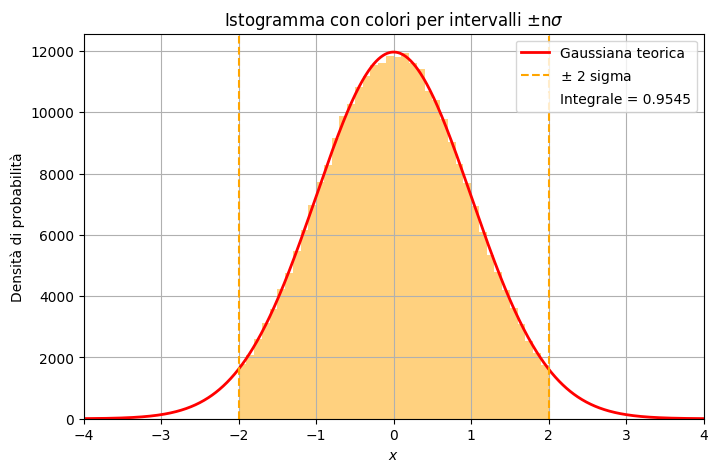
\includegraphics[width=0.7\textwidth]{Immagini/gauss_2sigma.png}
    \caption{Visualizzazione dell'area sottesa alla gaussiana standard nell'intervallo $\pm 2\sigma$. Come previsto dalla teoria, l'area copre circa il 95.4\% dei casi, un limite ben più stringente del 75\% garantito dalla disuguaglianza di Chebyshev.}
\end{figure}











Torniamo ora al caso della media $\bar{x}$ e applicando la disuguaglianza di prima avremo
\[
\text{Prob}(|\bar{x} - E[\bar{x}]| \ge \varepsilon) \le \frac{\text{Var}(\bar{x})}{\varepsilon^2}
\]
dove $E[\bar{x}] = E\left[ \frac{\sum_i x_i}{n} \right] = \frac{1}{n} \sum_i E[x_i] = \frac{1}{n} n\mu = \mu$ \\
mentre $\text{Var}(\bar{x}) = \text{Var}\left( \frac{1}{n} \sum_i x_i \right) = \frac{1}{n^2} \sum_i \text{Var}(x_i) = \frac{1}{n^2} n\sigma^2 = \frac{\sigma^2}{n}$ \\
Sostituendo si ha quindi
\[
\text{Prob}(|\bar{x} - \mu| \ge \varepsilon) \le \frac{\sigma^2}{n \varepsilon^2}
\]
Al limite per $n \to \infty$, $\frac{1}{n} \to 0$ per cui questo dimostra che
\[
\lim_{n \to \infty} \text{Prob}(|\bar{x} - \mu| \ge \varepsilon) = 0
\]

\vspace{0.5cm}
\noindent $\star \quad \text{Prob}(|X - \mu| \ge K\sigma) = 1 - \text{Prob}(|X - \mu| < K\sigma) \le \frac{1}{K^2}$ \\
$\implies \text{Prob}(|X - \mu| < K\sigma) \ge 1 - \frac{1}{K^2}$

\subsection{Cenni di Distribuzione Esponenziale}

\[
P_{\text{exp}}(x; \tau) = \frac{1}{\tau} e^{-x/\tau} \quad \quad 0 \le x \le +\infty
\]
Il valore di aspettazione e la varianza si calcolano facilmente dalla funzione generatrice dei momenti
\[
M_X(t) = E[e^{tx}] = \int_{0}^{\infty} e^{tx} \frac{1}{\tau} e^{-x/\tau} dx = \frac{1}{\tau} \int_{0}^{\infty} e^{(t - 1/\tau)x} dx
\]
\[
= \frac{1}{\tau} \frac{1}{t - 1/\tau} \left[ e^{(t - 1/\tau)x} \right]_0^\infty = \frac{1}{t\tau - 1} [0 - 1] = \frac{1}{1 - t\tau}
\]
Per calcolare il valore di aspettazione la derivo:
\[
M'_X(t) = \frac{-1}{(1 - t\tau)^2} (-\tau) = \frac{\tau}{(1 - t\tau)^2}
\]
\[
M'_X(0) = \tau = E[X]
\]
Calcolo la derivata seconda ($D(x^{-2}) = -2x^{-3}$)
\[
M''_X(t) = - \frac{2\tau}{(1 - t\tau)^3} (-\tau) = \frac{2\tau^2}{(1 - t\tau)^3}
\]
\[
M''_X(0) = 2\tau^2 = E[X^2]
\]
Ora calcolo la varianza come
\[
\text{Var}(X) = E[X^2] - (E[X])^2 = 2\tau^2 - \tau^2 = \tau^2
\]



\lezione{Processi di Poisson, Esponenziale ed Erlang}{19 Marzo 2026}

La distribuzione esponenziale descrive il tempo che intercorre tra due eventi consecutivi in un processo di Poisson.

Ricaviamola dalla \textbf{Distribuzione di Poisson}.
Se un fenomeno segue la \textbf{distribuzione di Poisson}, la probabilità di osservare $k$ eventi, dato un numero medio di eventi attesi $\nu$, è:
\begin{equation}
    P(k; \nu) = \frac{e^{-\nu} \nu^k}{k!}
\end{equation}

Se definiamo $\lambda$ come il numero di eventi attesi per \textbf{unità di tempo}, allora il numero medio di eventi attesi in un intervallo $t$ è $\lambda t$. La probabilità di osservare $k$ eventi nell'intervallo $t$ diventa:
\begin{equation}
    P(k; \lambda t) = \frac{e^{-\lambda t} (\lambda t)^k}{k!}
\end{equation}

Definiamo una nuova variabile casuale $T$ come l'intervallo di tempo che intercorre tra due eventi successivi.
Affinché il tempo di attesa $T$ sia maggiore di un certo valore $t$ ($T > t$), non deve verificarsi alcun evento nell'intervallo $[0, t]$.

Pertanto, la probabilità che $T > t$ coincide con la probabilità di osservare zero eventi nel periodo $t$:
\begin{equation}
    \text{Prob}(T > t) = P(0; \lambda t) = \frac{e^{-\lambda t} (\lambda t)^0}{0!} = e^{-\lambda t}
\end{equation}

\subsection{Richiami di Variabili casuali e CDF/PDF}
\ripasso{Variabili casuali e funzione di ripartizione}
Dato lo spazio di eventi elementare $\omega$ una \textit{variabile casuale} è una funzione $X$ tale che $X(\omega)=x$ dove $x\in$ R,
dunque una funzione che mi prende un campione casuale dal mio spazio campionario e gli associa un numero(ex: valore, altezza, \ldots).

Essa può essere discreta (numerabile) oppure continua, se almeno idealmente posso considerare $\Omega$ continuo.

\subsubsection{\color{red} Funzione di ripartizione}
Data una variabile casuale $X$, la funzione $F$ che fa corrispondere a un valore x la probabilità cumulativa $P(X \geq x)$ viene detta funzione di ripartizione

\[
F_X:\mathbf{R} \rightarrow [0,1] \; F_X(x)=P(X \leq x)
\]

La funzione di ripartizione è definita sia per le variabili casuali discrete che per le variabili casuali
continue.

Proprietà delle funzioni di ripartizioni:
\begin{enumerate}
    \item $0 \geq F_X(x) \geq 1$
    \item nel caso che il dominio sia \textbf{R}, allora $\displaystyle \lim_{x \rightarrow -\infty} F_X(x)=0 \; e \; \lim_{x \rightarrow \infty}F_X(x)=1$
    \item È una funzione monotona crescente;
    \item \( P(x_1 < X \leq x_2) = F_X(x_2) - F_X(x_1) \) dunque la funzione di ripartizione consente di stabilire la probabilità che la variabile casuale semplice \( X \) 
    assuma valori compresi in intervalli di tipo \((x_1, x_2]\) dove \( x_1, x_2 \in \mathbf{R} \), con \( x_1 < x_2 \). A partire da questo posso calcolare anche le altre probabilità, ad esempio:  
    \[ P(x_1 \leq X < x_2) = F_X(x_2) - F_X(x_1) + P(X = x_1) - P(X = x_2)\]
 
    \item Nel caso di una variabile casuale discreta, la funzione di ripartizione è continua a destra:  
    \[ \lim_{x \to x_0^+} F_X(x) = F_X(x_0).\]  
    mentre a sinistra abbiamo una discontinuità di 1° specie (o salto):  
    \[ \lim_{x \to x_0^-} F_X(x) \neq F_X(x_0)\]  
    Questo è dovuto al fatto che la probabilità di un evento elementare è diversa da zero, quindi la funzione di ripartizione ha un salto in corrispondenza di ogni valore che può assumere la variabile casuale discreta (pensa lancio dei dati dove cambia la probabilità)
\end{enumerate}

In un intervallo posso avere una \textbf{Probabilità uniforme}, ossia eventi in cui la funzione di probabilità è costante (ex nel caso dei dadi la funz. di ripartizione è a gradini)

\subsubsection{ \color{red} Densità di probabiità}

 Data la variabile casuale continua \( X: \Omega \to \mathbf{R} \) che associa valori dallo spazio campionario all'intervallo 
 \((a, b)\), con \( -\infty \leq a < b \leq +\infty \), la funzione di densità di probabilità (PDF) o funzione di distribuzione di probabilità è 
 la funzione \( f_X: \mathbf{R} \to \mathbf{R}^+ \) che ad ogni \( x \) associa il limite per \( dx \rightarrow 0\), del rapporto tra la probabilità 
 che la variabile casuale assuma valori nell'intervallo \((x, x + dx]\) e l'ampiezza \( dx \), ovverosia possiamo supporre la probabiità che un certo 
 evento cada in un intervallo.

 In simboli:
 
 \[ f_X: \mathbf{R} \to \mathbf{R}^+ : x \mapsto \lim_{dx \to 0} \left[ \frac{P(x < X \leq x + dx)}{dx} \right] = \lim_{dx \to 0} \frac{F_X(x+dx)- F_X(x)}{dx}\]

 Ogni evento deve essere ricondotto all'unione, negazione o intersezione di intervalli del tipo $( -\infty, x] $

 \textbf{Attenzione} a non confondere la funzione di densità con una probabilità.
 Essa mi determina la densità di probabilità che la variabile casuale sia nell'intervallo $dx$.

 Definimamo la \textbf{Funzione di distribuzione cumulativa}:
 \[
 F(x)=\int_{x_{min}}^x f_X(t)dt
 \]


\begin{center}
\begin{tikzpicture}[scale=1.5]
    
    % Asse x
    \draw[->] (-0.5,0) -- (4,0) node[right]{$x$};
    % Asse y
    \draw[->] (0,-0.5) -- (0,3) node[above]{$y$};
    
    % Etichette
    \node at (1.5,-0.2) {$a$};
    \node at (3,-0.2) {$b$};
    \node at (0.7,2.5) {$y = f_X(x)$};
    
    % Curva della PDF
    \draw[domain=0.5:3.5, smooth, variable=\x, blue] plot ({\x}, {2.5*exp(-0.5*(\x-2)^2)});
    
    % Area evidenziata
    \fill[blue!20] (1.5,0) -- plot[domain=1.5:3, smooth, variable=\x] ({\x}, {2.5*exp(-0.5*(\x-2)^2)}) -- (3,0) -- cycle;
    
    % Linee verticali
    \draw[dashed] (1.5,0) -- (1.5,{2.5*exp(-0.5*(1.5-2)^2)});
    \draw[dashed] (3,0) -- (3,{2.5*exp(-0.5*(3-2)^2)});
    
    % Etichetta probabilità
    \node at (2.25,0.7) {$P(a \leq X \leq b)=\int_{a}^{b}f_X(x)dx$};
\end{tikzpicture}
\end{center}

\subsubsection*{Proprietà della funzione densità di probabilità}
\begin{itemize}
    \item non può essere mai negativa (altrimenti avremmo una probabiità negativa per qualche $X$)
    \item condizione di normalizzazione: \[ \int_{- \infty}^{\infty} f(x)=1\]
    dunque si deve avere che: $\lim_{x \rightarrow \pm \infty} f_X(x)=0$
    \item la probabilità che una variabile casuale assuma un particolare valore dell'intervallo è $P(X=x)=0$, infatti ad un singolo valore corrisponde un intervallo con ampiezza nulla; questo mi porta a poter escludere gli estremi
\end{itemize}

\subsection{Proprietà dell'Esponenziale}
La \textbf{funzione di ripartizione} (o distribuzione cumulativa $F_X(x)$) indica la probabilità che una variabile $x'$ assuma un valore minore o uguale a $x$:
\begin{equation}
    F_X(x) = \text{Prob}(x' \le x) = \int_{-\infty}^{x} P_X(z) \, dz
\end{equation}
Dalle proprietà della probabilità, segue la normalizzazione: $\int_{-\infty}^{+\infty} P_X(x) \, dx = 1$.

Per la variabile tempo $T$, la funzione di ripartizione è:
\begin{equation}
    F_T(t) = \text{Prob}(T \le t) = 1 - \text{Prob}(T > t) = 1 - e^{-\lambda t}
\end{equation}

La \textbf{densità di probabilità} $P_T(t)$ si ottiene derivando la funzione di ripartizione:
\begin{equation}
    P_T(t) = \frac{d}{dt} F_T(t) = \frac{d}{dt} (1 - e^{-\lambda t}) = \lambda e^{-\lambda t}
\end{equation}
Questa è la densità di probabilità esponenziale. Indica che i tempi di attesa brevi sono più probabili, mentre quelli lunghi sono meno probabili.


\begin{figure}[ht!]
    \centering
    \begin{tikzpicture}
        \begin{axis}[
            standard,
            ylabel={$P(t), F(t)$},
            title={Confronto tra PDF e CDF Esponenziale ($\lambda=1$)},
            legend pos=north east
        ]
            \addplot [very thick, red, domain=0:4] {exp(-x)};
            \addlegendentry{PDF: $\lambda e^{-\lambda t}$}
            \addplot [very thick, blue, domain=0:4] {1 - exp(-x)};
            \addlegendentry{CDF: $1 - e^{-\lambda t}$}
            \draw [dashed, gray] (axis cs:0,1) -- (axis cs:4,1);
        \end{axis}
    \end{tikzpicture}
    \caption{La PDF decresce partendo da $\lambda$, mentre la CDF satura asintoticamente a 1.}
\end{figure}


\subsubsection*{Proprietà di Assenza di Memoria}
Una caratteristica fondamentale è l'\textbf{assenza di memoria}: il tempo che resta da aspettare affinché un evento si verifichi è indipendente da quanto abbiamo già aspettato.
Usando la probabilità condizionata $\text{Prob}(A|M) = \frac{\text{Prob}(A \cap M)}{\text{Prob}(M)}$:
\begin{itemize}
    \item $s$: tempo già aspettato.
    \item $t$: tempo addizionale da aspettare.
    \item $A \rightarrow T > s + t$
    \item $M \rightarrow T > s$
\end{itemize}
\begin{equation}
    \text{Prob}(T > s+t \mid T > s) = \frac{\text{Prob}(T > s+t)}{\text{Prob}(T > s)} = \frac{e^{-\lambda(s+t)}}{e^{-\lambda s}} = e^{-\lambda t} = P(T > t)
\end{equation}

\paragraph{Parametrizzazione con $\tau$}
Spesso si scrive la distribuzione utilizzando $\tau = 1/\lambda$, dove $\tau$ rappresenta il \textbf{tempo medio} tra due eventi (mentre $\lambda$ è la frequenza):
\begin{equation}
    P_{exp}(x; \tau) = \frac{1}{\tau} e^{-x/\tau} \quad \text{per } 0 \le x \le +\infty
\end{equation}



\subsection{Distribuzione di Erlang}
La distribuzione di Erlang è una generalizzazione della distribuzione esponenziale. Mentre l'esponenziale regola il tempo tra due eventi successivi ($k=1$), la distribuzione di Erlang regola il tempo di attesa per il \textbf{k-esimo evento}.



Sia $T_k$ il tempo di attesa fino al $k$-esimo evento.
\begin{itemize}
    \item $P_1(t; \lambda) = \lambda e^{-\lambda t}$ (Esponenziale)
    \item Per $P_2$, supponiamo che il primo evento avvenga a $x$ ($0 < x < t$) e il secondo nel tempo restante $t-x$:
\end{itemize}
\begin{equation}
    P_2(t; \lambda) = \int_0^t P_1(x; \lambda) P_1(t-x; \lambda) \, dx = \int_0^t \lambda e^{-\lambda x} \lambda e^{-\lambda(t-x)} \, dx = \lambda^2 t e^{-\lambda t}
\end{equation}

Procedendo per induzione per $P_3$:
\begin{equation}
    P_3(t; \lambda) = \int_0^t P_2(x; \lambda) P_1(t-x; \lambda) \, dx = \int_0^t \lambda^2 x e^{-\lambda x} \lambda e^{-\lambda(t-x)} \, dx = \frac{t^2}{2} \lambda^3 e^{-\lambda t}
\end{equation}




\begin{figure}[ht!]
    \centering
    \begin{tikzpicture}[scale=1.2]
        \draw[thick, ->] (0,0) -- (6,0) node[right]{$t$};
        \filldraw (0,0) circle (2pt) node[below]{$0$};
        \filldraw (2.5,0) circle (2pt) node[below]{$x$ (1° evento)};
        \filldraw (5,0) circle (2pt) node[below]{$t$ (2° evento)};
        
        \draw [decorate, decoration={brace, amplitude=6pt, raise=5pt}] (0,0) -- (2.5,0) node [midway, above=12pt] {$x$};
        \draw [decorate, decoration={brace, amplitude=6pt, raise=5pt}] (2.5,0) -- (5,0) node [midway, above=12pt] {$t-x$};
        \draw [decorate, decoration={brace, mirror, amplitude=10pt, raise=25pt}] (0,0) -- (5,0) node [midway, below=35pt] {$T_2 = t$};
    \end{tikzpicture}
    \caption{Schema temporale per il calcolo della distribuzione di Erlang $P_2$.}
\end{figure}


Continuando ricorsivamente, si ottiene la densità di probabilità di Erlang:
\begin{equation}
    P_k(t; \lambda) = \frac{t^{k-1}}{(k-1)!} \lambda^k e^{-\lambda t}
\end{equation}

\textbf{Momenti della distribuzione:}
\begin{itemize}
    \item Valore di aspettazione: $E[t] = \frac{k}{\lambda}$
    \item Varianza: $Var(t) = \frac{k}{\lambda^2}$
\end{itemize}

\subsubsection{Distribuzione Gamma}
Cosideriamo $\alpha$ e $\beta$ due costati maggiori di zero, allora la \textit{Gamma distribution} è definita come:
\begin{equation}
    f(x;\alpha,\beta)= \frac{1}{\Gamma(\alpha)\beta^\alpha}x^{\alpha-1}e^{-\frac{x}{\beta}} \label{eq: pdf Gamma}
\end{equation}
con la condizione di $0 \leqq x < \infty$.\\
Questa risulta normalizzata in base alla condizione sulla funzione gamma:
\begin{equation*}
    \Gamma(\alpha)= \int_{0}^{\infty} y^{\alpha-1} e^{-y} dy
\end{equation*}
con la condizione di $\alpha >0$; ricordiamo per correttezza la proprietà della funzione Gamma:
\begin{equation*}
    \Gamma(\alpha)= (\alpha -1 ) \gamma(\alpha -1)
\end{equation*}
\begin{figure}[htbp]
    \centering
    \includegraphics[width=0.7\textwidth]{Immagini/gamma_shapes.png}
    \caption{Al variare del parametro $\alpha$ trovo diverse pdf, il fattore $\beta$ rappresenta un riscalamento}
\end{figure} 
Nel caso in cui $\alpha \in\mathbb{N}$, vado a ritrovare la \textit{distribuzione di Erlang} 




\section{Metodi Monte Carlo}
I metodi Monte Carlo sono algoritmi computazionali che sfruttano la generazione di numeri casuali per risolvere problemi matematici complessi.
Questo campionamento casuale ha un certo numero di applicazioni, ma una delle più utili è che consente
di calcolare in modo pratico integrali altrimenti impossibili.  
\paragraph{Esempio}
Per calcolare l'area di una superficie irregolare:\\
1. Si lancia un numero $N$ di chicchi di riso a caso su un foglio di area nota. \\
2. Si conta quanti chicchi cadono dentro l'area cercata ($N_{in}$).\\
3. Il rapporto $N_{in}/N$ fornisce una stima dell'area, che diventa più accurata al crescere di $N$.

\subsection{Metodo Accept-Reject}
È un metodo generale per generare variabili continue secondo una distribuzione $f(x)$ non standard.
Dati un intervallo $[x_{min}, x_{max}]$ e un valore massimo della funzione $f_{max}$:
\begin{enumerate}
    \item Si genera $x_i$ con distribuzione uniforme tra $x_{min}$ e $x_{max}$: $x_i = x_{min} + r_1 (x_{max} - x_{min})$.
    \item Si genera $y_i$ con distribuzione uniforme tra 0 e $f_{max}$.
    \item Se $y_i < f(x_i)$, si \textbf{accetta} il valore $x_i$; altrimenti lo si rifiuta.
\end{enumerate}
L'efficienza $\eta$ è il rapporto tra l'area sotto $f(x)$ e l'area del rettangolo:
\begin{equation}
    \eta = \frac{1}{(x_{max} - x_{min}) f_{max}} \int_{x_{min}}^{x_{max}} f(x) \, dx
\end{equation}

\paragraph{Esempio: Algoritmo Hit-or-Miss in Python}
Il seguente script implementa il metodo Accept-Reject per campionare una distribuzione di probabilità legata allo scattering angolare (distribuzione di Cowen): $f(x) = \frac{3}{8}(1+x^2)$.

\begin{lstlisting}[language=Python, caption={Implementazione del metodo Accept-Reject}]
import numpy as np
import matplotlib.pyplot as plt

def mia_funz(x):
    return 3/8*(1+x**2)

# Parametri del dominio e numero di punti
xmin, xmax = -1, 1
fmax = 3/4
N = 5000

accepted_x, accepted_y = [], []
rejected_x, rejected_y = [], []

# Ciclo Accept-Reject
while len(accepted_x) < N:
    x = np.random.uniform(xmin, xmax)
    y = np.random.uniform(0, fmax)

    if y <= mia_funz(x):
        accepted_x.append(x)
        accepted_y.append(y)
    else:
        rejected_x.append(x)
        rejected_y.append(y)

# Visualizzazione dei risultati
plt.figure(figsize=(8,6))
x_plot = np.linspace(xmin, xmax, 400)
plt.plot(x_plot, mia_funz(x_plot), label='f(x) teorica', lw=3)
plt.scatter(accepted_x, accepted_y, color='tab:green', s=4, label='Accettati')
plt.scatter(rejected_x, rejected_y, color='tab:red', s=4, label='Rifiutati')
plt.legend()
plt.show()
\end{lstlisting}

\begin{figure}[H]
    \centering
    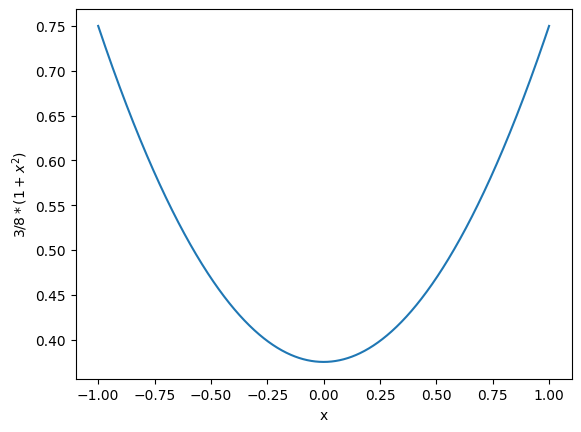
\includegraphics[width=0.6\textwidth]{Immagini/plot della funzione.png}
    \caption{Andamento della funzione teorica $f(x) = \frac{3}{8}(1+x^2)$ nell'intervallo $[-1, 1]$.}
\end{figure}

\begin{figure}[H]
    \centering
    
\includegraphics[width=0.8\textwidth]{immagini/funzione con accept reject.png}
    \caption{Visualizzazione del metodo Hit-or-Miss: i punti in verde sono accettati perché cadono sotto la curva, quelli in rosso sono rifiutati.}
\end{figure}

\begin{figure}[H]
    \centering
    
\includegraphics[width=0.8\textwidth]{immagini/confronto distribuzione tra f(x) teorica e campioni.png}
    \caption{Validazione del metodo: l'istogramma dei punti accettati segue fedelmente la curva teorica attesa (punti arancioni).}
\end{figure}



\subsection{Metodo della Funzione di Ripartizione (Inversione)}
Un metodo più efficiente dell'Accept-Reject si basa sull'inversione della CDF.
Dato che $F(x) = \int_{-\infty}^x P(z) \, dz$ ha valori compresi tra 0 e 1, se generiamo un numero casuale $u \sim \mathcal{U}(0,1)$, allora:
\begin{equation}
    x = F^{-1}(u)
\end{equation}
Il valore $x$ così ottenuto sarà distribuito secondo la $P(x)$ originale.

\textbf{Esempio per la distribuzione esponenziale:}
\begin{itemize}
    \item $P(x) = \frac{1}{\tau} \exp(-\frac{x}{\tau})$
    \item $F(x) = 1 - \exp(-\frac{x}{\tau}) = u$
    \item Invertendo: $x =   -\tau \ln(1 - u)$
\end{itemize}


\paragraph{Esempio: Integrazione Numerica e CDF}
Questo script mostra come calcolare numericamente la funzione di ripartizione (CDF) partendo dalla densità di probabilità (PDF) e come visualizzare il legame tra le due.

\begin{lstlisting}[language=Python, caption={Integrazione numerica della Gaussiana e PDF/CDF Esponenziale}]
import numpy as np
import matplotlib.pyplot as plt
import math

# Funzione densita di probabilita (PDF) Gaussiana
def gaussian_pdf(x, mu=0, sigma=1):
    return (1 / (sigma * math.sqrt(2 * math.pi))) * np.exp(-((x - mu) ** 2) / (2 * sigma ** 2))

# Integrazione numerica con il metodo dei rettangoli
def integra(a, b, n=200000):
    base = (b - a) / n
    somma = 0.0
    for k in range(n):
        x_mid = a + (k + 0.5) * base
        somma += gaussian_pdf(x_mid)
    return base * somma

# Esempio probabilita entro sigma
for s in [1, 2, 3]:
    area = integra(-s, s)
    print(f"Probabilita entro {s} sigma: {area:.6f}")

# Plot PDF e CDF per una distribuzione esponenziale
tau = 5
x_axis = np.arange(0, 30, 0.1)
func_exp = np.exp(-x_axis/tau)/tau
cum_exp = 1 - np.exp(-x_axis/tau)

fig, axes = plt.subplots(1, 2, figsize=(12, 5))
axes[0].plot(x_axis, func_exp, label='PDF Esponenziale')
axes[1].plot(x_axis, cum_exp, label='CDF Esponenziale', color='orange')
plt.show()
\end{lstlisting}



\begin{figure}[ht!]
    \centering
    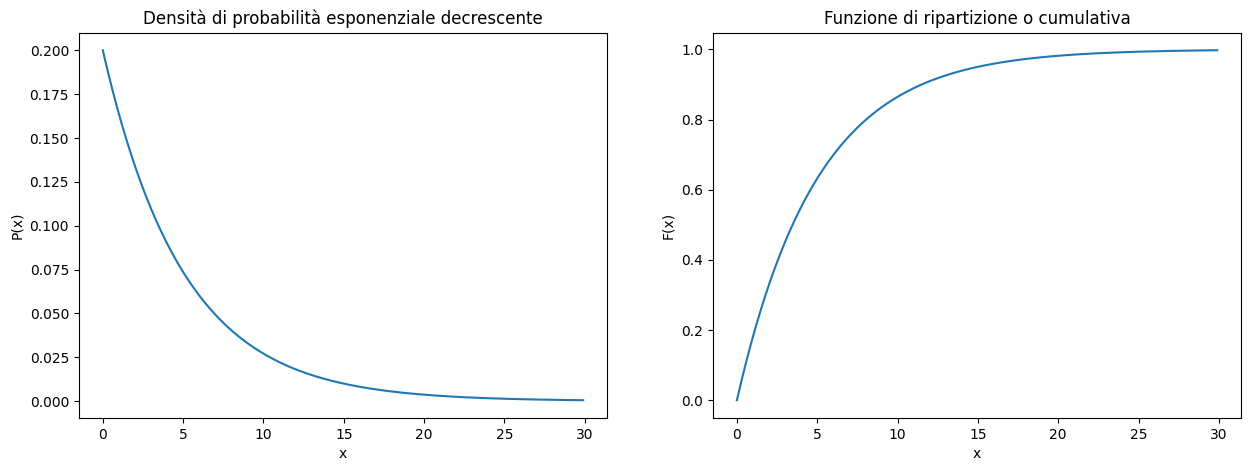
\includegraphics[width=0.9\textwidth]{Immagini/Funzione d ripartizione cumulativa e densità di probabilità esponenziale decrescente.png}
    \caption{Densità di probabilità (sinistra) e Funzione di ripartizione (destra) per la distribuzione esponenziale generata dal codice Python.}
    \label{fig:esponenziale_plot}
\end{figure}

\begin{figure}[ht!]
    \centering
    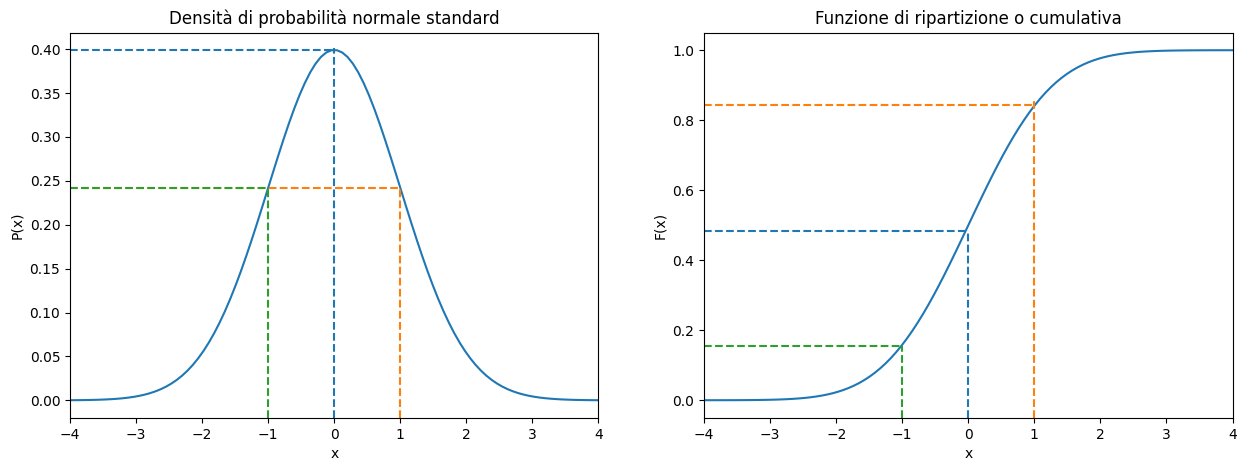
\includegraphics[width=0.9\textwidth]{Immagini/Funzione di ripartizione cumulativa e Densità di probabilità normale standard.png}
    \caption{Analisi della distribuzione normale: PDF (sinistra) e CDF (destra). Le linee tratteggiate indicano i valori corrispondenti a $\pm 1 \sigma$.}
    \label{fig:gauss_plot}
\end{figure}

\pagebreak  

%------------------------------------------------------------------------------

\lezione{Variabili Casuali bidimensionali}{23/03/2026}
\subsection{Distribuzioni congiunte, marginali e condizionate}
Abbiamo già accennato ad alcune proprietà delle distribuzioni di più variabili, adesso concentriamoci sul caso più semplice di distribuzione di più variabili, ovvero quando le variabili sono due.\\
Supponiamo allora di avere una coppia di variabili aleatorie $X$ e $Y$ (caso di un esperimento in cui si misurano due quantità).
\\
La \textbf{densità di probabilità congiunta} $P(x,y)$ indica la probabilità che una certa realizzazione $X$ di $x$ e una certa realizzazione $Y$ di $y$ abbiano valori, rispettivamente, in $(x, x+dx)$ e $(y, y+dy)$ per $dx \to 0$ e $dy \to 0$.
\\
Come nel caso unidimensionale, si può usare $P(x,y)$ per definire altre funzioni, per esempio la \textbf{funzione di distribuzione congiunta}:
\begin{equation}
    F(x,y) = \int_{-\infty}^{x} du \int_{-\infty}^{y} dv \, P(u,v) = Prob(X \le x, Y \le y)
\end{equation}
che indica la probabilità di ottenere valori delle due variabili non superiori a quantità prefissate $x, y$. A partire dalla $F(x,y)$ si può scrivere la condizione di normalizzazione come $F(+\infty, +\infty) = 1$, cioè:
\begin{equation}
    \int_{-\infty}^{+\infty} dx \int_{-\infty}^{+\infty} dy \, P(x,y) = 1
\end{equation}


A partire da $P(x,y)$ si può calcolare la densità di probabilità per una delle due variabili \textit{qualunque valore abbia l'altra}, cioè le funzioni di \textbf{distribuzioni marginali}:
\begin{equation}
    P_X(x) = \int_{-\infty}^{+\infty} P(x,y) \,dy \quad \text{e} \quad P_Y(y) = \int_{-\infty}^{+\infty} P(x,y) \,dx
\end{equation}

Altre distribuzioni che si definiscono nel caso di più variabili sono le \textbf{funzioni di distribuzione condizionate}, che rappresentano la densità di probabilità dei valori di una variabile fissato il valore dell'altra, che indicheremo con $\prod(x|y)$ e $\prod(y|x)$. La cui espressione si può ricavare dal calcolo:
\begin{equation}
    P(x,y)\,dx\,dy = P_X(x)\,dx \cdot \prod(y|x)\,dy = P_Y(y)\,dy \cdot \prod(x|y)\,dx
\end{equation}
Si ha quindi:
\begin{equation}
    \prod(y|x) = \frac{P(x,y)}{P_X(x)} \quad \text{e} \quad \prod(x|y) = \frac{P(x,y)}{P_Y(y)}
\end{equation}

Nel caso in cui $X$ e $Y$ siano \textbf{indipendenti}, allora aver fissato il valore di una variabile non dovrebbe alterare la distribuzione dell'altra, cioè ci aspettiamo che sia:
\begin{equation}
    \prod(x|y) = P_X(x) \quad \text{e} \quad \prod(y|x) = P_Y(y)
\end{equation}
Se sostituiamo in una delle equazioni precedenti, per esempio in $\pi(y|x) = P(x,y)/P_X(x)$, abbiamo:
\begin{equation}
    P_Y(y) = \frac{P(x,y)}{P_X(x)} \implies P(x,y) = P_X(x)P_Y(y)
\end{equation}



\subsection{Momenti: Matrice delle Covarianze e Combinazioni Lineari}

Come nel caso unidimensionale si può calcolare il valore di aspettazione, però stavolta per generalizzare, considero una qualunque funzione di $x$ e $y$, $f(x,y)$, e definisco il suo \textbf{valore di aspettazione} come:
\begin{equation}
    \mathbb{E}[f(x,y)] = \int_{-\infty}^{+\infty} \,dx \int_{-\infty}^{+\infty} \,dy \, f(x,y) P(x,y)
\end{equation}

A partire da ciò posso definire i \textbf{momenti rispetto all'origine} come:
\begin{equation}
    \mu_{mn} = \mathbb{E}[X^m Y^n]
\end{equation}
per cui:
\begin{align*}
    \mu_{00} &= \mathbb{E}[1] = \int_{-\infty}^{+\infty} \,dx \int_{-\infty}^{+\infty} \,dy \, P(x,y) = 1 \\
    \mu_{10} &= \mathbb{E}[X] \\
    \mu_{01} &= \mathbb{E}[Y]
\end{align*}

Analogamente è possibile definire i \textbf{momenti rispetto al valore di aspettazione} di $X$ e $Y$ (momenti centrali) come:
\begin{equation}
    \bar{\mu}_{mn} = \mathbb{E}\left[ (X - \mathbb{E}[X])^m (Y - \mathbb{E}[Y])^n \right]
\end{equation}
dove i più notevoli sono:
\begin{align*}
    \bar{\mu}_{20} &= \mathbb{E}\left[ (X - \mathbb{E}[X])^2 \right] = \text{Var}(X) \\
    \bar{\mu}_{02} &= \mathbb{E}\left[ (Y - \mathbb{E}[Y])^2 \right] = \text{Var}(Y) \\
    \bar{\mu}_{11} &= \mathbb{E}\left[ (X - \mathbb{E}[X])(Y - \mathbb{E}[Y]) \right] = \text{Cov}(X,Y)
\end{align*}

Quest'ultima quantità si chiama \textbf{covarianza} ed è un parametro importante nel caso di più variabili perché \textit{indica come sono correlate fra loro le variabili}. Infatti si può dimostrare che $\text{Cov}(X,Y) = 0$ se $X$ e $Y$ sono indipendenti l'una dall'altra.

\subsubsection*{Dimostrazione nel caso discreto}
Per dimostrarlo è conveniente trovare un altro modo di scrivere la covarianza che si ricava più facilmente assumendo il caso discreto.
Consideriamo il caso di 2 variabili discrete $X$ e $Y$; il valore di aspettazione di una determinata funzione è dato da: 
\[
\mathbb{E}[f(x,y] = \sum_{i,j} P_{X,Y}(x_i,y_i)f(x_i,y_i)
\]

dunque la covarianza è descrivibile da:

\begin{align*}
    \text{Cov}(X,Y) &= \mathbb{E}\left[ (X - \mathbb{E}[X])(Y - \mathbb{E}[Y]) \right] = \text{caso discreto} \\
    &= \sum_{i,j} P_{ij} (x_i - \mathbb{E}[X])(y_j - \mathbb{E}[Y]) = \quad \text{(svolgo il prodotto)} \\
    &= \sum_{i,j} P_{ij} x_i y_j - \sum_{i,j} P_{ij} x_i \mathbb{E}[Y] - \sum_{i,j} P_{ij} y_j \mathbb{E}[X] + \sum_{i,j} P_{ij} \mathbb{E}[X]\mathbb{E}[Y]
\end{align*}

Riconosciamo i vari termini:
\begin{itemize}
    \item $\sum_{i,j} P_{ij} x_i y_j = $ valore di aspettazione del prodotto $XY = \mathbb{E}[XY]$
    \item $\sum_{i,j} P_{ij} x_i = \mathbb{E}[X]$
    \item $\sum_{i,j} P_{ij} y_j = \mathbb{E}[Y]$
    \item $\sum_{i,j} P_{ij} \mathbb{E}[X]\mathbb{E}[Y] = \mathbb{E}[X]\mathbb{E}[Y] \sum_{i,j} P_{ij} = \mathbb{E}[X]\mathbb{E}[Y] \cdot 1 = \mathbb{E}[X]\mathbb{E}[Y]$
\end{itemize}

Quindi mettendo tutto insieme:
\begin{align}
    \text{Cov}(X,Y) &= \mathbb{E}[XY] - \mathbb{E}[X]\mathbb{E}[Y] - \mathbb{E}[Y]\mathbb{E}[X] + \mathbb{E}[X]\mathbb{E}[Y] \nonumber \\
              &= \mathbb{E}[XY] - \mathbb{E}[X]\mathbb{E}[Y]
\end{align}

Questa formula vale in generale, ma nel caso in cui le variabili siano indipendenti allora nella sommatoria il termine $P_{ij}$ si può scrivere come prodotto di un termine che dipende solo da $i$ (che indico con $P_{X,i}$) e un termine che dipende solo da $j$ (che indico con $P_{Y,j}$), in analogia a $P(x,y)=P_X(x)P_Y(y)$. Quindi:
\begin{equation*}
    \mathbb{E}[XY] = \sum_{i,j} P_{ij} x_i y_j = \sum_{i,j} P_{X,i} x_i P_{Y,j} y_j = \mathbb{E}[X]\mathbb{E}[Y]
\end{equation*}
Di conseguenza, in questo caso, $\text{Cov}(X,Y) = 0$.
\subsubsection*{Matrice delle covarianze (e combinazioni lineari di variabili)}

Quando si lavora con più variabili si costruisce di solito la matrice delle covarianze che serve a semplificare la notazione. Il tipico esempio che fa capire da dove salta fuori è il calcolo del valore di aspettazione e varianza per una nuova variabile ottenuta come combinazione lineare di altre variabili.

Il caso più semplice è quello di $Z = aX + bY$, dove $a$ e $b$ sono degli scalari e $X$ e $Y$ sono due variabili aleatorie che per semplicità supponiamo abbiano $\mathbb{E}[X] = \mathbb{E}[Y] = 0$.
Il valore di aspettazione di $Z$ vale:
\begin{equation*}
    \mathbb{E}[Z] = a\mathbb{E}[X] + b\mathbb{E}[Y] = 0
\end{equation*}

La varianza di $Z$ vale:
\begin{align*}
    \text{Var}(Z) &= \mathbb{E}[(Z - \mathbb{E}[Z])^2] = \mathbb{E}[Z^2] = \mathbb{E}[(aX + bY)^2] = \\
            &= \mathbb{E}[a^2 X^2] + \mathbb{E}[b^2 Y^2] + \mathbb{E}[2abXY] = \\
            &= a^2 \mathbb{E}[X^2] + b^2 \mathbb{E}[Y^2] + 2ab \mathbb{E}[XY]
\end{align*}
il che si può scrivere in funzione delle varianze e della covarianza dato che $\mathbb{E}[X]=\mathbb{E}[Y]=0$, cioè:
\begin{equation}
\boxed{
    \text{Var}(Z) = a^2 \text{Var}(X) + b^2 \text{Var}(Y) + 2ab \text{Cov}(X,Y)}
\end{equation}

Il risultato sulla varianza si può generalizzare al caso in cui $\mathbb{E}[X] \neq 0$ e $\mathbb{E}[Y] \neq 0$ perché basta fare il cambiamento di variabili $X' = X - \mathbb{E}[X]$ e $Y' = Y - \mathbb{E}[Y]$ che evidentemente hanno $\mathbb{E}[X'] = 0$ e $\mathbb{E}[Y'] = 0$. Inoltre:
\begin{equation*}
    \text{Var}(X') = \text{Var}(X - \mathbb{E}[X]) = \text{Var}(X)
\end{equation*}
(aggiungere o sottrarre una costante a una variabile non altera la varianza). Analogamente $\text{Var}(Y') = \text{Var}(Y)$, e infine si ha che:
\begin{equation*}
    \text{Cov}(X', Y') = \mathbb{E}\left[ (X' - \mathbb{E}[X'])(Y' - \mathbb{E}[Y']) \right] = \mathbb{E}\left[ (X - \mathbb{E}[X])(Y - \mathbb{E}[Y]) \right] = \text{Cov}(X,Y)
\end{equation*}
Quindi anche se le variabili non hanno valore di aspettazione nullo vale la stessa formula per $\text{Var}(Z)$.

\subsubsection*{Formulazione Matriciale}
Risulta utile esprimere questo risultato sotto forma di moltiplicazioni di matrici (soprattutto quando si estende a più dimensioni) ed è a questo punto che si definisce la \textbf{matrice delle covarianze} (che è simmetrica) come:
\begin{equation}
    V = \begin{pmatrix}
    \text{Var}(X) & \text{Cov}(X,Y) \\
    \text{Cov}(X,Y) & \text{Var}(Y)
    \end{pmatrix}
\end{equation}
Quindi $V$ ha nella diagonale principale le varianze e nelle altre le covarianze. Si definisce poi la matrice dei coefficienti $A = \begin{pmatrix} a \\ b \end{pmatrix}$, la cui trasposta è $A^T = (a \quad b)$, in modo che la formula di prima si può scrivere come:
\begin{equation}
    \text{Var}(Z) = A^T V A
\end{equation}

\begin{nota}
Ci si convince abbastanza facilmente del risultato se si fa il conto:
\begin{align*}
    (a \quad b) \begin{pmatrix} \text{Var}(X) & \text{Cov}(X,Y) \\ \text{Cov}(X,Y) & \text{Var}(Y) \end{pmatrix} \begin{pmatrix} a \\ b \end{pmatrix} 
    &= \big[ a\text{Var}(X) + b\text{Cov}(X,Y) \quad a\text{Cov}(X,Y) + b\text{Var}(Y) \big] \begin{pmatrix} a \\ b \end{pmatrix} \\
    &= a^2 \text{Var}(X) + ab \text{Cov}(X,Y) + ab \text{Cov}(X,Y) + b^2 \text{Var}(Y)
\end{align*}

Si può poi ancora di più generalizzare al caso di $N$ variabili aleatorie $X_i$ come $Z = \sum_{i=1}^{N} a_i X_i$, e avremo ancora $\text{Var}(Z) = A^T V A$, dove stavolta la matrice delle covarianze ha elementi $V_{ij} = \text{Cov}(X_i, X_j)$. Essendo la diagonale:
\begin{equation*}
    V_{ii} = \text{Cov}(X_i, X_i) = \mathbb{E}\left[ (X_i - \mathbb{E}[X_i])(X_i - \mathbb{E}[X_i]) \right] = \mathbb{E}\left[ (X_i - \mathbb{E}[X_i])^2 \right] = \text{Var}(X_i)
\end{equation*}
Quindi $V$ è qualcosa come:
\begin{equation}
    V = \begin{pmatrix}
    \text{Var}(X_1) & \text{Cov}(X_1, X_2) & \cdots & \text{Cov}(X_1, X_N) \\
    \text{Cov}(X_2, X_1) & \text{Var}(X_2) & \cdots & \text{Cov}(X_2, X_N) \\
    \vdots & \vdots & \ddots & \vdots \\
    \text{Cov}(X_N, X_1) & \text{Cov}(X_N, X_2) & \cdots & \text{Var}(X_N)
    \end{pmatrix}
\end{equation}
mentre la matrice $A = \begin{pmatrix} a_1 \\ a_2 \\ \vdots \\ a_N \end{pmatrix}$.
È chiaro che se le variabili $X_i$ sono indipendenti allora $V$ assume una forma molto semplice in cui gli elementi non nulli sono solo nella diagonale.
\end{nota}


\subsection{Coefficiente di correlazione}

Una ultima quantità che si introduce parlando del caso di due variabili casuali $X$ e $Y$ è il \textbf{coefficiente di correlazione lineare} ( che indica  la forza e la direzione della relazione lineare tra due variabili) definito come:

\begin{equation}
\boxed{
    \rho = \frac{\text{Cov}(X,Y)}{\sqrt{\text{Var}(X) \cdot \text{Var}(Y)}} = \frac{\text{Cov}(X,Y)}{\sigma_X \sigma_Y}
}
\end{equation}


È chiaro dalla definizione che $\rho$ è \textbf{adimensionale} (mentre la covarianza non lo è!), che $\rho = 0$ se $X$ e $Y$ sono statisticamente indipendenti (visto che in tal caso $\text{Cov}(X,Y)=0$), e si può dimostrare che:
\begin{equation}
    -1 \le \rho \le 1
\end{equation}

\textbf{Dimostrazione:} Esistono vari modi per dimostrarlo, una possibilità è definire la variabile $Z = \sigma_Y X - \sigma_X Y$ e calcolare $\text{Var}(Z)$ sfruttando la formula precedente:
\begin{equation*}
    \text{Var}(Z) = \sigma_Y^2 \text{Var}(X) + \sigma_X^2 \text{Var}(Y) - 2\sigma_X \sigma_Y \text{Cov}(X,Y)
\end{equation*}
ma $\text{Var}(X) = \sigma_X^2$ e $\text{Var}(Y) = \sigma_Y^2$, quindi:
\begin{equation*}
    \text{Var}(Z) = 2\sigma_X^2 \sigma_Y^2 - 2\sigma_X \sigma_Y \text{Cov}(X,Y)
\end{equation*}
Per come è definita sappiamo che $\text{Var}(Z) \ge 0$, quindi:
\begin{align*}
    & 2\sigma_X^2 \sigma_Y^2 - 2\sigma_X \sigma_Y \text{Cov}(X,Y) \ge 0 \\
    \implies & \sigma_X^2 \sigma_Y^2 \ge \sigma_X \sigma_Y \text{Cov}(X,Y) \\
    \implies & \frac{\text{Cov}(X,Y)}{\sigma_X \sigma_Y} \le 1 \implies \rho \le 1
\end{align*}
Viceversa se si definisce $Z = \sigma_Y X + \sigma_X Y$ e si fa lo stesso conto si trova $\rho \ge -1$.


\begin{example}
È istruttivo vedere quanto vale $\rho$ nel caso di due variabili legate da una relazione lineare come $Y = mX + q$, cioè l'equazione della retta. In questo caso si può calcolare $\rho$ partendo da:
\begin{itemize}
    \item $\mathbb{E}[Y] = m\mathbb{E}[X] + q$
    \item $\text{Var}(Y) = m^2 \text{Var}(X)$
    \item $\mathbb{E}[XY] = \mathbb{E}[X(mX + q)] = \mathbb{E}[mX^2 + qX] = m\mathbb{E}[X^2] + q\mathbb{E}[X]$
    \item $\text{Cov}(X,Y) = \mathbb{E}[XY] - \mathbb{E}[X]\mathbb{E}[Y] = \\
          = m\mathbb{E}[X^2] + q\mathbb{E}[X] - \mathbb{E}[X]\big(m\mathbb{E}[X] + q\big) = \\
          = m\mathbb{E}[X^2] + q\mathbb{E}[X] - m\{\mathbb{E}[X]\}^2 - q\mathbb{E}[X] = \\
          = m\left( \mathbb{E}[X^2] - \{\mathbb{E}[X]\}^2 \right) = m\text{Var}(X)$
\end{itemize}
Premesso questo posso calcolare $\rho$ come:
\begin{equation}
    \rho = \frac{\text{Cov}(X,Y)}{\sqrt{\text{Var}(X)\text{Var}(Y)}} = \frac{m \text{Var}(X)}{\sqrt{m^2 [\text{Var}(X)]^2}} = \frac{m}{|m|} = \pm 1
\end{equation}
Quindi $\rho$ vale $1$ con il \textit{segno} del coefficiente angolare della retta. Questo mostra che man mano che la relazione tra $X$ e $Y$ approssima una relazione lineare il valore di $|\rho|$ si avvicina a 1.

\end{example}


\subsubsection*{Visualizzazione dei casi}

% Disegno dei grafici di correlazione con TikZ
\begin{center}
\begin{tikzpicture}[scale=0.8]
    % rho = 0
    \begin{scope}[shift={(0,0)}]
        \draw[->, thick] (0,-0.2) -- (0,3) node[left] {$Y$};
        \draw[->, thick] (-0.2,0) -- (3,0) node[below] {$X$};
        \node at (2,2.5) {$\rho = 0$};
        \foreach \i in {1,...,50} {\filldraw (rand*0.8+1.5, rand*0.8+1.5) circle (1pt);}
    \end{scope}
    
    % rho > 0
    \begin{scope}[shift={(5,0)}]
        \draw[->, thick] (0,-0.2) -- (0,3) node[left] {$Y$};
        \draw[->, thick] (-0.2,0) -- (3,0) node[below] {$X$};
        \node at (2,2.5) {$\rho > 0$};
        \foreach \i in {1,...,40} {\filldraw (rand*0.6+1.5, {rand*0.6+1.5 + (\i*0.01 - 0.2)}) circle (1pt);}
        % Approximation of positive slope cloud
        \fill [white] (0,0) rectangle (3,3); % clear area to redraw accurately
        \draw[->, thick] (0,-0.2) -- (0,3) node[left] {$Y$};
        \draw[->, thick] (-0.2,0) -- (3,0) node[below] {$X$};
        \node at (2,2.5) {$\rho > 0$};
        \foreach \i in {1,...,60} {
            \pgfmathsetmacro{\x}{rand*0.7+1.5}
            \pgfmathsetmacro{\y}{\x*0.8 + rand*0.4 + 0.2}
            \filldraw (\x,\y) circle (1pt);
        }
    \end{scope}

    % rho < 0
    \begin{scope}[shift={(10,0)}]
        \draw[->, thick] (0,-0.2) -- (0,3) node[left] {$Y$};
        \draw[->, thick] (-0.2,0) -- (3,0) node[below] {$X$};
        \node at (2.5,2.5) {$\rho < 0$};
        \foreach \i in {1,...,60} {
            \pgfmathsetmacro{\x}{rand*0.7+1.5}
            \pgfmathsetmacro{\y}{-\x*0.7 + rand*0.4 + 2.5}
            \filldraw (\x,\y) circle (1pt);
        }
    \end{scope}

    % rho ~ 1
    \begin{scope}[shift={(2.5,-4)}]
        \draw[->, thick] (0,-0.2) -- (0,3) node[left] {$Y$};
        \draw[->, thick] (-0.2,0) -- (3,0) node[below] {$X$};
        \node at (2.5,2) {$\rho \sim 1$};
        \foreach \i in {1,...,40} {
            \pgfmathsetmacro{\x}{\i*0.06 + 0.3}
            \pgfmathsetmacro{\y}{\x + rand*0.1}
            \filldraw (\x,\y) circle (1pt);
        }
    \end{scope}

    % rho ~ -1
    \begin{scope}[shift={(7.5,-4)}]
        \draw[->, thick] (0,-0.2) -- (0,3) node[left] {$Y$};
        \draw[->, thick] (-0.2,0) -- (3,0) node[below] {$X$};
        \node at (2.5,2) {$\rho \sim -1$};
        \foreach \i in {1,...,40} {
            \pgfmathsetmacro{\x}{\i*0.06 + 0.3}
            \pgfmathsetmacro{\y}{-\x*1.1 + 3 + rand*0.1}
            \ifdim \y pt > 0 pt
                \filldraw (\x,\y) circle (1pt);
            \fi
        }
    \end{scope}
\end{tikzpicture}
\end{center}

Come in precedenza, quanto detto per due variabili si può facilmente estendere al caso di $N$ variabili $X_i$, e in tal caso il coefficiente di correlazione si calcola comunque per una coppia delle $N$ variabili:
\begin{equation}
    \rho_{ij} = \frac{\text{Cov}(X_i, X_j)}{\sigma_i \sigma_j}
\end{equation}
Si noti anche che da questo segue che $\text{Cov}(X_i, X_j) = \sigma_i \sigma_j \rho_{ij}$ e quindi la matrice delle covarianze si può anche scrivere come:
\begin{equation}
    V_{ij} = \sigma_i \sigma_j \rho_{ij}
\end{equation}

\subsection*{(Approfondimento facoltativo: Significato quantitativo di $\rho$) \footnote{Fonte: John R. Taylor, \textit{Introduzione all'analisi degli errori - Lo studio delle incertezze nelle misure fisiche}, 3\textsuperscript{a} ed., Bologna, Zanichelli Editore SpA, 2023}}



Finora abbiamo definito il coefficiente di correlazione e le sue proprietà teoriche. Tuttavia, in un caso reale, ci si trova sempre a lavorare con un \textbf{campione finito} di $N$ coppie di misure $(x_i, y_i)$. 
\\
\\
Supponiamo di calcolare il coefficiente di correlazione per i nostri dati misurati e di ottenere un valore, che chiameremo $\rho_{oss}$ (correlazione \textit{osservata}), per esempio $\rho_{oss} = 0,8$. La domanda sorge spontanea: \textit{questo valore è sufficiente per affermare con certezza che le variabili sono correlate linearmente?}
\\
\\
Per rispondere, dobbiamo fare un ragionamento al contrario, basato sul calcolo delle probabilità. Supponiamo che le variabili $X$ e $Y$ siano in realtà \textbf{completamente non correlate} (ovvero, nel limite di infinite misure avremmo $\rho = 0$). Poiché abbiamo effettuato solo un numero finito $N$ di misure, è quasi impossibile che il calcolo dia esattamente $0$; per puro caso, i dati mostreranno sempre una qualche correlazione spuria. 

Si definisce quindi la probabilità:
\begin{equation}
    P_N(|\rho| \ge |\rho_{oss}|)
\end{equation}
che rappresenta la probabilità che $N$ misure di due variabili \textit{non correlate} producano, per puro caso, un coefficiente di correlazione in valore assoluto grande almeno quanto quello osservato. 

\begin{itemize}
    \item Se questa probabilità è \textbf{alta}, il valore $\rho_{oss}$ ottenuto potrebbe benissimo essere frutto del caso. Non abbiamo prove di una vera correlazione.
    \item Se questa probabilità è \textbf{bassa}, è estremamente improbabile che variabili scorrelate abbiano prodotto quel valore. Concludiamo quindi che le variabili sono quasi certamente correlate.
\end{itemize}

Per convenzione, si considera una correlazione:
\begin{itemize}
    \item \textbf{Significativa:} se la probabilità è $\le 5\%$
    \item \textbf{Altamente significativa:} se la probabilità è $\le 1\%$
\end{itemize}

Il calcolo esatto di queste probabilità è complesso, ma i risultati per alcuni valori rappresentativi sono riportati nella tabella seguente:

\begin{table}[h!]
    \centering
    \caption{Probabilità percentuale $P_N(|\rho| \ge |\rho_{oss}|)$ che $N$ misure di due variabili non correlate producano un coefficiente di correlazione $\ge |\rho_{oss}|$. Gli spazi vuoti indicano valori inferiori allo $0,05\%$.}
    \vspace{2mm}
    \renewcommand{\arraystretch}{1.2} % Migliora la spaziatura verticale delle righe
    \begin{tabular}{c | c c c c c c c c c c c}
        \hline
        & \multicolumn{11}{c}{$|\rho_{oss}|$} \\
        $N$ & $0$ & $0,1$ & $0,2$ & $0,3$ & $0,4$ & $0,5$ & $0,6$ & $0,7$ & $0,8$ & $0,9$ & $1$ \\
        \hline
        3  & 100 & 94 & 87 & 81 & 74  & 67 & 59  & 51  & 41  & 29 & 0 \\
        6  & 100 & 85 & 70 & 56 & 43  & 31 & 21  & 12  & 6   & 1  & 0 \\
        10 & 100 & 78 & 58 & 40 & 25  & 14 & 7   & 2   & 0,5 &    & 0 \\
        20 & 100 & 67 & 40 & 20 & 8   & 2  & 0,5 & 0,1 &     &    & 0 \\
        50 & 100 & 49 & 16 & 3  & 0,4 &    &     &     &     &    & 0 \\
        \hline
    \end{tabular}
\end{table}

\begin{example}
Facendo riferimento alla tabella, si può notare come il numero di dati $N$ influenzi drasticamente la significatività di un risultato. Supponiamo di aver calcolato un coefficiente $\rho_{oss} = 0,7$:
\begin{itemize}
    \item Con sole \textbf{$N=3$} misure, la probabilità che variabili totalmente scorrelate diano $|\rho| \ge 0,7$ per puro caso è del \textbf{51\%}. Il risultato non dimostra assolutamente nulla.
    \item Con \textbf{$N=6$} misure, la probabilità scende al \textbf{12\%}. La situazione migliora, ma non è ancora considerabile "significativa" (siamo sopra la soglia del 5\%).
    \item Con \textbf{$N=20$} misure, la probabilità crolla allo \textbf{0,1\%}. In questo caso l'evidenza è fortissima ("altamente significativa"): possiamo escludere quasi con certezza che le variabili non siano correlate.
\end{itemize}
In sintesi, un coefficiente di correlazione non ha significato pratico se non viene contestualizzato rispetto al numero di misurazioni effettuate.
\end{example}

\section{Distribuzione normale in più dimensioni (o multinormale)}
\subsection{Caso di variabili indipendenti}
La distribuzione gaussiana che abbiamo visto in una dimensione si può estendere al caso di due o più dimensioni partendo dal caso più semplice in cui le variabili sono indipendenti. Supponiamo quindi che $X$ abbia densità di probabilità:
\begin{equation}
    P_X(x) = \frac{1}{\sigma_X \sqrt{2\pi}} \exp\left[ -\frac{(x-\mu_X)^2}{2\sigma_X^2} \right]
\end{equation}
e analogamente $Y$ ha densità di probabilità:
\begin{equation}
    P_Y(y) = \frac{1}{\sigma_Y \sqrt{2\pi}} \exp\left[ -\frac{(y-\mu_Y)^2}{2\sigma_Y^2} \right]
\end{equation}

Essendo indipendenti, la densità di probabilità congiunta sarà:
\begin{align*}
    P(x,y) &= P_X(x) P_Y(y) \\
           &= \frac{1}{2\pi \sigma_X \sigma_Y} \exp\left[ -\frac{(x-\mu_X)^2}{2\sigma_X^2} \right] \cdot \exp\left[ -\frac{(y-\mu_Y)^2}{2\sigma_Y^2} \right]
\end{align*}
Essendo $e^a e^b = e^{a+b}$ posso riscrivere come:
\begin{equation}
    P(x,y) = \frac{1}{2\pi \sigma_X \sigma_Y} \cdot \exp\left\{ -\left[ \frac{(x-\mu_X)^2}{2\sigma_X^2} + \frac{(y-\mu_Y)^2}{2\sigma_Y^2} \right] \right\}
\end{equation}
Se si definisce la quantità:
\begin{equation}
    Q^2 = \frac{(x-\mu_X)^2}{\sigma_X^2} + \frac{(y-\mu_Y)^2}{\sigma_Y^2}
\end{equation}
allora si può riscrivere la probabilità come:
\begin{equation}
    P(x,y) = \frac{1}{2\pi \sigma_X \sigma_Y} \cdot \exp\left( -\frac{Q^2}{2} \right)
\end{equation}

La definizione di $Q^2$ è utile perché le intersezioni di $P(x,y)$ con piani paralleli al piano $XY$ sono definite proprio dall'equazione $Q^2 = \text{costante}$. Questo si capisce facilmente perché occorre fare l'intersezione con il piano $Z=K$, quindi servono valori di $X$ e $Y$ tali che $P(x,y) = K$, ma l'unica dipendenza da $X$ e $Y$ è contenuta in $Q$, per il resto si tratta di costanti:
\begin{align*}
    \frac{1}{2\pi \sigma_X \sigma_Y} \exp\left( -\frac{Q^2}{2} \right) &= K \\
    \exp\left( -\frac{Q^2}{2} \right) &= K \, 2\pi \sigma_X \sigma_Y \\
    -\frac{Q^2}{2} &= \ln(2\pi \sigma_X \sigma_Y K) \\
    Q^2 &= -2\ln(2\pi \sigma_X \sigma_Y K) = C
\end{align*}
Scrivendo esplicitamente si ha:
\begin{equation}
    \frac{(x-\mu_X)^2}{\sigma_X^2} + \frac{(y-\mu_Y)^2}{\sigma_Y^2} = C
\end{equation}
che è l'equazione di un'\textbf{ellisse centrata in} $(\mu_X, \mu_Y)$.


\begin{figure}[h]
    \centering
    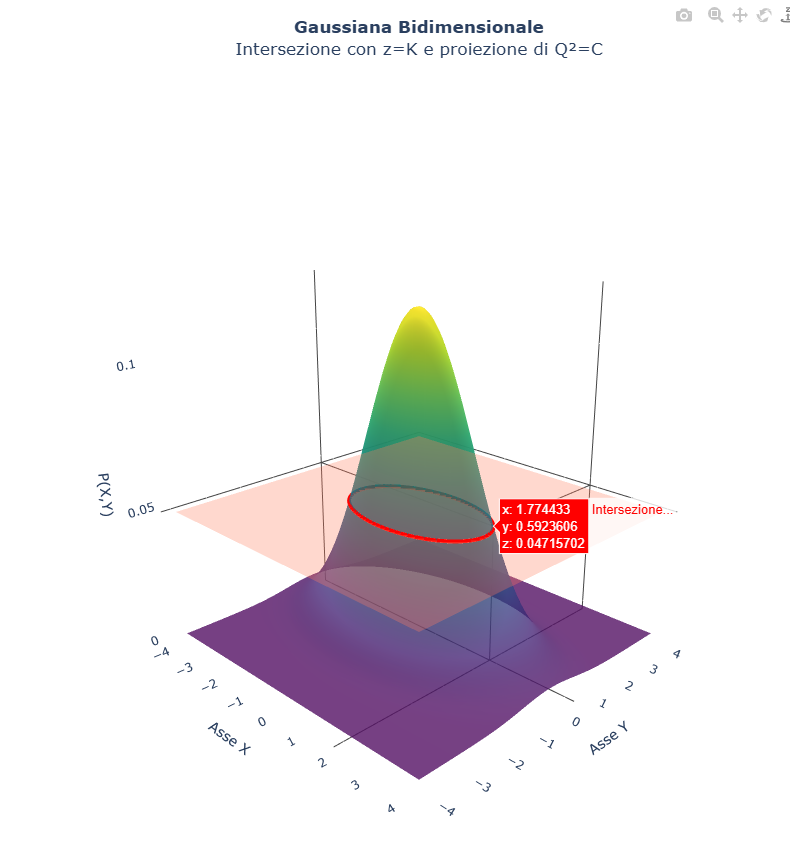
\includegraphics[width=0.8\textwidth]{Immagini/gaussiana_3d.png}
    \caption{Rappresentazione 3D della densità di probabilità congiunta. La linea rossa rappresenta l'intersezione con il piano $z=K$, la cui proiezione sul piano $XY$ è un'ellisse di equazione $Q^2 = C$. Per provare il grafico interattivo: \url{https://colab.research.google.com/drive/1mZmU06E-0UsUTA-w0U_cUEBHEPlPrn5u?usp=sharing}}
    \label{fig:gaussiana_3d}
\end{figure}




Essendo $Q^2$ dato dalla somma di quadrati di variabili normali, si può dimostrare che la sua distribuzione di probabilità è una distribuzione notevole che si chiama \textbf{distribuzione del chi quadro}, indicata con $\chi^2$, che vedremo meglio più avanti. Per ora quello che  è utile sapere è che si può calcolare, per ogni valore di $C$, la probabilità che il generico punto $(X,Y)$ cada dentro l'ellisse $Q^2 \le C$. 

Per esempio, per $C=1$ (il che equivale al caso in cui l'ellisse ha come semiassi $\sigma_X$ e $\sigma_Y$) si vede che tale probabilità è \textbf{0.39}.

\begin{center}
\begin{tikzpicture}[scale=1.5]
    % Assi
    \draw[->, thick] (0,-0.5) -- (0,3) node[left] {$Y$};
    \draw[->, thick] (-0.5,0) -- (4,0) node[below] {$X$};
    
    % Centro
    \filldraw (2,1.5) circle (1pt);
    \node[below] at (2,0) {$\mu_X$};
    \node[left] at (0,1.5) {$\mu_Y$};
    \draw[dashed] (2,0) -- (2,1.5) -- (0,1.5);
    
    % Ellisse
    \draw[thick] (2,1.5) ellipse (1.2cm and 0.8cm);
    
    % Rettangolo circoscritto
    \draw[dashed] (0.8, 0.7) rectangle (3.2, 2.3);
    
    % Etichette su X
    \draw (0.8, 0.1) -- (0.8, -0.1) node[below] {$\mu_X - \sigma_X$};
    \draw (3.2, 0.1) -- (3.2, -0.1) node[below] {$\mu_X + \sigma_X$};
    
    % Etichette su Y
    \draw (0.1, 0.7) -- (-0.1, 0.7) node[left] {$\mu_Y - \sigma_Y$};
    \draw (0.1, 2.3) -- (-0.1, 2.3) node[left] {$\mu_Y + \sigma_Y$};
\end{tikzpicture}
\end{center}

Si noti che se io considerassi il rettangolo che circoscrive l'ellisse, mi aspetterei \footnote{Ricordando che integrando la gaussiana entro un sigma ottengo una probabilità del 68\%}:
\begin{align*}
    \text{Prob}\Big( \mu_X - \sigma_X \le X \le \mu_X + \sigma_X \ &\&\ \mu_Y - \sigma_Y \le Y \le \mu_Y + \sigma_Y \Big) = \\
    &= 0.68 \cdot 0.68 = 0.46
\end{align*}

In maniera analoga è facile graficamente intuire che forma avranno le \textbf{densità di probabilità condizionate} $\prod(x|y)$ e $\prod(y|x)$: nel caso di variabili indipendenti saranno ancora delle gaussiane e rappresentano le intersezioni con i piani del tipo $X = \text{costante}$ e $Y = \text{costante}$.










\lezione{Distribuzione Multi-normale (Variabili dipendenti)}{26 Marzo 2026}
\subsection*{Richiamo al caso di variabili indipendenti}
Abbiamo visto che per due variabili indipendenti con distribuzione normale si trova:
\begin{equation}
P(x,y) = \frac{1}{2\pi\sigma_x\sigma_y} \cdot \exp\left(-\frac{Q^2}{2}\right)
\end{equation}
essendo la forma quadratica $Q^2$ definita come:
\begin{equation}
Q^2 = \frac{(x-\mu_x)^2}{\sigma_x^2} + \frac{(y-\mu_y)^2}{\sigma_y^2}
\end{equation}

Per estendere il discorso al caso di variabili \emph{correlate}, è utile esprimere $Q^2$ sotto forma di prodotto di matrici usando la \textbf{matrice delle covarianze} $V$, che per due variabili indipendenti ha la forma diagonale:
\begin{equation}
V = \begin{pmatrix}
\sigma_x^2 & 0 \\
0 & \sigma_y^2
\end{pmatrix}
\end{equation}

Se si indicano i vettori colonna:
\begin{equation*}
\vec{x} = \begin{pmatrix} x \\ y \end{pmatrix} \quad \text{e} \quad \vec{\mu} = \begin{pmatrix} \mu_x \\ \mu_y \end{pmatrix}
\end{equation*}

allora si vede che la rappresentazione compatta di $Q^2$ è:
\begin{equation}
Q^2 = (\vec{x} - \vec{\mu})^T V^{-1} (\vec{x} - \vec{\mu})
\end{equation}

Questo si può verificare facilmente ricavando innanzitutto quanto vale $V^{-1}$. Ricordiamo che per una generica matrice $2 \times 2$ del tipo $M = \begin{pmatrix} a & b \\ c & d \end{pmatrix}$, la sua inversa è $M^{-1} = \frac{1}{\det M} \begin{pmatrix} d & -b \\ -c & a \end{pmatrix}$. 
Nel nostro caso, $\det V = \sigma_x^2 \sigma_y^2$, quindi:
\begin{equation}
V^{-1} = \frac{1}{\sigma_x^2\sigma_y^2} \begin{pmatrix} \sigma_y^2 & 0 \\ 0 & \sigma_x^2 \end{pmatrix} = \begin{pmatrix} \sigma_x^{-2} & 0 \\ 0 & \sigma_y^{-2} \end{pmatrix}
\end{equation}

Sostituendo si ottiene esattamente l'espressione nota di $Q^2$:
\begin{align*}
(\vec{x} - \vec{\mu})^T V^{-1} (\vec{x} - \vec{\mu}) &= \begin{pmatrix} x-\mu_x & y-\mu_y \end{pmatrix} \begin{pmatrix} \sigma_x^{-2} & 0 \\ 0 & \sigma_y^{-2} \end{pmatrix} \begin{pmatrix} x-\mu_x \\ y-\mu_y \end{pmatrix} \\
&= \begin{pmatrix} \frac{x-\mu_x}{\sigma_x^2} & \frac{y-\mu_y}{\sigma_y^2} \end{pmatrix} \begin{pmatrix} x-\mu_x \\ y-\mu_y \end{pmatrix} \\
&= \frac{(x-\mu_x)^2}{\sigma_x^2} + \frac{(y-\mu_y)^2}{\sigma_y^2} = Q^2
\end{align*}

\subsection*{Generalizzazione a $n$ dimensioni}
Mettendo tutto insieme ed estendendo al caso di $n$ dimensioni (e usando $\det V$ al posto di $\sigma_x^2\sigma_y^2$), si ottiene l'espressione generale:
\begin{equation}
P(\vec{x}) = \frac{1}{(2\pi)^{n/2} |\det V|^{1/2}} \exp\left[ -\frac{1}{2}(\vec{x}-\vec{\mu})^T V^{-1} (\vec{x}-\vec{\mu}) \right]
\end{equation}

\subsection*{Il caso binormale correlato}
Scritta così, l'espressione vale \emph{anche nel caso in cui le variabili non siano indipendenti}. Ritornando al caso particolare di 2 variabili, la matrice $V$ assume la forma:
\begin{equation}
V = \begin{pmatrix}
\text{var}(x) & \text{cov}(x,y) \\
\text{cov}(x,y) & \text{var}(y)
\end{pmatrix} = \begin{pmatrix}
\sigma_x^2 & \rho \sigma_x \sigma_y \\
\rho \sigma_x \sigma_y & \sigma_y^2
\end{pmatrix}
\end{equation}

Il suo determinante è:
\begin{equation}
\det V = \sigma_x^2 \sigma_y^2 - \rho^2 \sigma_x^2 \sigma_y^2 = \sigma_x^2 \sigma_y^2 (1 - \rho^2)
\end{equation}

Per calcolare $Q^2$ bisogna calcolare $V^{-1}$, che in questo caso vale:
\begin{equation}
V^{-1} = \frac{1}{\sigma_x^2\sigma_y^2(1-\rho^2)} \begin{pmatrix}
\sigma_y^2 & -\rho\sigma_x\sigma_y \\
-\rho\sigma_x\sigma_y & \sigma_x^2
\end{pmatrix}
\end{equation}

Svolgendo tutti i calcoli matriciali, si trova la forma quadratica espansa:
\begin{equation}
Q^2 = \frac{1}{1-\rho^2} \left[ \frac{(x-\mu_x)^2}{\sigma_x^2} - 2\rho\frac{(x-\mu_x)(y-\mu_y)}{\sigma_x\sigma_y} + \frac{(y-\mu_y)^2}{\sigma_y^2} \right]
\end{equation}
E la gaussiana in 2D diventa:
\begin{equation}
P(x,y) = \frac{1}{2\pi\sigma_x\sigma_y\sqrt{1-\rho^2}} \exp\left(-\frac{Q^2}{2}\right)
\end{equation}

\subsection{Interpretazione geometrica: L'ellisse}
La cosa interessante è che ponendo $Q^2 = c$ si ottiene ancora un'ellisse, ma stavolta è \emph{inclinata}, cioè non ha gli assi paralleli agli assi cartesiani $x$ ed $y$.

Data la geometria del problema, dalla forma dell'ellisse si potrebbe riuscire a ricavare $\rho$. Infatti:
\begin{itemize}
    \item La retta $x = \mu_x$ interseca l'ellisse nei punti di coordinate $y = \mu_y \pm \sigma_y\sqrt{1-\rho^2}$.
    \item La retta $y = \mu_y$ interseca l'ellisse nei punti di coordinate $x = \mu_x \pm \sigma_x\sqrt{1-\rho^2}$.
\end{itemize}

Invece, le rette di equazione $x = \mu_x \pm \sigma_x$ (parallele all'asse $y$) sono tangenti all'ellisse, e i punti di intersezione/tangenza hanno coordinate $y = \mu_y \pm \sigma_y\rho$.
Analogamente, le rette $y = \mu_y \pm \sigma_y$ sono tangenti all'ellisse nei punti di coordinate $x = \mu_x \pm \rho\sigma_x$.

\begin{nota}
Anche in questo caso, la probabilità che una misurazione $(x,y)$ cada dentro l'ellisse $Q^2 \leq 1$ è approssimativamente $0.39$.
\end{nota}
\begin{figure}[htbp]
\centering
\begin{tikzpicture}[scale=1.2, every node/.style={scale=0.9}]
    
    % Assi cartesiani principali
    \draw[->, thick] (-1, 0) -- (9, 0) node[right] {$x$};
    \draw[->, thick] (0, -1) -- (0, 6.5) node[above] {$y$};

    % --- Parametri usati per il disegno ---
    % \mu_x = 4, \mu_y = 3
    % \sigma_x = 3, \sigma_y = 2
    % \rho = 0.6  (il che implica \sqrt{1-\rho^2} = 0.8)
    
    % Rettangolo di contenimento (Bounding box) corrispondente a \mu \pm \sigma
    \draw[dashed, gray] (1, 1) rectangle (7, 5);
    
    % Proiezioni della bounding box sugli assi cartesiani
    \draw[dashed, gray] (1, 1) -- (1, 0) node[below] {$\mu_x - \sigma_x$};
    \draw[dashed, gray] (7, 1) -- (7, 0) node[below] {$\mu_x + \sigma_x$};
    \draw[dashed, gray] (1, 1) -- (0, 1) node[left] {$\mu_y - \sigma_y$};
    \draw[dashed, gray] (1, 5) -- (0, 5) node[left] {$\mu_y + \sigma_y$};
    
    % Rette passanti per il centro (\mu_x, \mu_y)
    \draw[dashed, darkgray] (4, 0) node[below] {$\mu_x$} -- (4, 6);
    \draw[dashed, darkgray] (0, 3) node[left] {$\mu_y$} -- (8, 3);

    % --- Disegno dell'Ellisse ---
    % Equazione parametrica esatta derivata dalla forma quadratica Q^2 = 1
    % x(t) = \mu_x + \sigma_x \cos(t)
    % y(t) = \mu_y + \sigma_y (\rho \cos(t) + \sqrt{1-\rho^2} \sin(t))
    \draw[thick, blue, domain=0:360, samples=100] 
        plot ({4 + 3*cos(\x)}, {3 + 2*(0.6*cos(\x) + 0.8*sin(\x))});
        
    % --- Punti di tangenza con il bounding box (Rossi, come negli appunti) ---
    \filldraw[red] (7, 4.2) circle (2pt);   % Tangenza destra
    \filldraw[red] (1, 1.8) circle (2pt);   % Tangenza sinistra
    \filldraw[red] (5.8, 5) circle (2pt);   % Tangenza superiore
    \filldraw[red] (2.2, 1) circle (2pt);   % Tangenza inferiore
    
    % --- Punti di intersezione con le medie (Neri) ---
    \filldraw[black] (6.4, 3) circle (2pt); % Intersezione asse \mu_y (destra)
    \filldraw[black] (1.6, 3) circle (2pt); % Intersezione asse \mu_y (sinistra)
    \filldraw[black] (4, 4.6) circle (2pt); % Intersezione asse \mu_x (sopra)
    \filldraw[black] (4, 1.4) circle (2pt); % Intersezione asse \mu_x (sotto)

    % --- Frecce e Quote per indicare le distanze ---
    % Distanza: \sigma_x \sqrt{1-\rho^2}
    \draw[<->, >=stealth] (4, 3.2) -- (6.4, 3.2) 
        node[midway, above, font=\footnotesize] {$\sigma_x\sqrt{1-\rho^2}$};
        
    % Distanza: \rho \sigma_x
    \draw[<->, >=stealth] (4, 5.2) -- (5.8, 5.2) 
        node[midway, above, font=\footnotesize] {$\rho\sigma_x$};
        
    % Distanza: \sigma_y \sqrt{1-\rho^2}
    \draw[<->, >=stealth] (4.2, 3) -- (4.2, 4.6) 
        node[midway, right, font=\footnotesize] {$\sigma_y\sqrt{1-\rho^2}$};
        
    % Distanza: \rho \sigma_y
    \draw[<->, >=stealth] (7.2, 3) -- (7.2, 4.2) 
        node[midway, right, font=\footnotesize] {$\rho\sigma_y$};

\end{tikzpicture}
\caption{Rappresentazione geometrica dell'ellisse di equazione $Q^2 = c$. Si notano le intersezioni con gli assi passanti per il centro e i punti di tangenza con il box $\mu \pm \sigma$, che permettono di ricavare visivamente il coefficiente di correlazione $\rho$.}
\label{fig:ellisse_covarianza}
\end{figure}


\subsection{Distribuzioni Marginali e Condizionate per la Multinormale}

Per definizione, le distribuzioni marginali sono date da:
\begin{equation}
P_x(x) = \int_{-\infty}^{+\infty} P(x,y) \, dy \quad \text{e} \quad P_y(y) = \int_{-\infty}^{+\infty} P(x,y) \, dx
\end{equation}

Nel caso in cui $x$ e $y$ siano \textbf{indipendenti}, per una binormale è ovvio che $P_x(x)$ e $P_y(y)$ rappresentano le singole gaussiane. Infatti:
\begin{equation*}
P_x(x) = \int_{-\infty}^{+\infty} P_x(x)P_y(y) \, dy = P_x(x) \underbrace{\int_{-\infty}^{+\infty} P_y(y) \, dy}_{=1} = P_x(x)
\end{equation*}
Quindi $P_x(x) = \mathcal{N}(\mu_x, \sigma_x^2)$ e $P_y(y) = \mathcal{N}(\mu_y, \sigma_y^2)$.

Se $x$ e $y$ \textbf{non sono indipendenti}, si arriva allo stesso risultato ma con più passaggi. La sostanza del calcolo si basa sul fatto che $Q^2$ dipende dai quadrati dei termini $(x-\mu_x)^2$ e $(y-\mu_y)^2$; con un po' di passaggi algebrici si riescono ad ottenere due gaussiane.

\subsubsection*{Distribuzioni Condizionate}
È più istruttivo calcolare con più dettaglio le \textbf{distribuzioni condizionate}. Si vede che anche queste sono gaussiane, ma con $\mu$ e $\sigma$ alterati da $\rho$.
Dalla definizione sappiamo che:
\begin{equation}
\pi(x|y) = \frac{P(x,y)}{P_y(y)} = \frac{F \exp[-Q^2/2]}{F_1 \exp[-Q_1^2/2]}
\end{equation}
dove abbiamo scritto schematicamente le probabilità come prodotto di un fattore di normalizzazione ($F$ e $F_1$) per degli esponenziali, ponendo $Q_1^2 = \frac{(y-\mu_y)^2}{\sigma_y^2}$.

Il calcolo più facile da fare è il rapporto dei coefficienti:
\begin{equation}
\frac{F}{F_1} = \frac{\frac{1}{2\pi\sigma_x\sigma_y\sqrt{1-\rho^2}}}{\frac{1}{\sqrt{2\pi}\sigma_y}} = \frac{1}{\sqrt{2\pi}\sigma_x\sqrt{1-\rho^2}}
\end{equation}
Da questo si nota che per avere la forma di una gaussiana normalizzata, la nuova deviazione standard deve essere:
\begin{equation}
\sigma_{x|y} = \sigma_x \sqrt{1-\rho^2}
\end{equation}
(Si noti che per $\rho = 0$ si ritrova $\sigma_{x|y} = \sigma_x$).

\subsubsection*{Calcolo della media condizionata}
Per ricavare come varia $\mu$ bisogna calcolare come varia l'esponente. Per semplificare la notazione utilizziamo il cambiamento di variabili:
$u = x - \mu_x$ e $v = y - \mu_y$.

Con questa scelta, il rapporto tra i due esponenziali è dipendente da:
\begin{equation*}
Q^2 - Q_1^2 = \frac{1}{1-\rho^2} \left( \frac{u^2}{\sigma_x^2} + \frac{v^2}{\sigma_y^2} - 2\rho\frac{uv}{\sigma_x\sigma_y} \right) - \frac{v^2}{\sigma_y^2}
\end{equation*}

Separiamo i termini che dipendono da $x$ (cioè $u$) e quelli che dipendono solo da $y$ (cioè $v$):
\begin{align*}
Q^2 - Q_1^2 &= \frac{1}{1-\rho^2} \left( \frac{u^2}{\sigma_x^2} - 2\rho\frac{uv}{\sigma_x\sigma_y} \right) - \left[ \frac{1}{1-\rho^2} - 1 \right] \frac{v^2}{\sigma_y^2} \\
\end{align*}
Riscriviamo il termine in parentesi quadra come un quadrato di binomio mettendo in evidenza $\frac{1}{\sigma_x^2}$:
\begin{equation*}
\frac{1}{\sigma_x^2} (u^2 - 2\rho\frac{\sigma_x}{\sigma_y}uv) = \frac{1}{\sigma_x^2} \left[ \left(u - \rho\frac{\sigma_x}{\sigma_y}v\right)^2 - \rho^2\frac{\sigma_x^2}{\sigma_y^2}v^2 \right]
\end{equation*}

Sostituendo nell'espressione precedente e semplificando i termini in $v^2$:
\begin{align*}
Q^2 - Q_1^2 &= \frac{1}{1-\rho^2} \left[ \frac{1}{\sigma_x^2} \left( u - \rho\frac{\sigma_x}{\sigma_y}v \right)^2 - \rho^2\frac{v^2}{\sigma_y^2} + \rho^2\frac{v^2}{\sigma_y^2} \right] \\
&= \frac{1}{(1-\rho^2)\sigma_x^2} \left( u - \rho\frac{\sigma_x}{\sigma_y}v \right)^2
\end{align*}

Tornando alle variabili originarie $x$ e $y$:
\begin{equation}
Q^2 - Q_1^2 = \frac{1}{(1-\rho^2)\sigma_x^2} \left\{ \left(x-\mu_x\right) - \rho\frac{\sigma_x}{\sigma_y}(y-\mu_y) \right\}^2
\end{equation}

Da qui si evince che l'espressione di $\pi(x|y)$ è ancora una gaussiana con deviazione standard $\sigma_{x|y} = \sigma_x\sqrt{1-\rho^2}$ (come visto prima) e con valore atteso:
\begin{equation}
\mu_{x|y} = \mu_x + \rho\frac{\sigma_x}{\sigma_y}(y-\mu_y)
\end{equation}
Anche in questo caso, se $\rho = 0$ si ha $\mu_{x|y} = \mu_x$, mentre se $\rho \neq 0$, il valore atteso è spostato rispetto al valore $\mu_x$ originale in base al valore di $y$.


\section{Teoria della Stima dei Parametri}

Finora abbiamo parlato molto di distribuzioni teoriche, ma il problema che ci si trova spesso ad affrontare è trovare un modo di risalire ai \textbf{parametri della distribuzione della popolazione}, dato un insieme di misure di un campione.

Detto in maniera più formale, supponiamo che la densità di probabilità $P(x;\theta)$ di una variabile casuale $x$ dipenda da un parametro $\theta$, il cui \textbf{valore vero} $\theta_v$ ci sia ignoto (per esempio, se $P$ è una gaussiana, avremo due parametri: $\mu$ e $\sigma$).

Avendo a disposizione $N$ misure $x_i$ della grandezza $x$, vogliamo trovare una funzione:
\begin{equation*}
\hat{\theta} = \hat{\theta}(x_1, x_2, \dots, x_N)
\end{equation*}
che, a partire da esse, ci permetta di ricavare il valore di $\theta_v$. Le funzioni $\hat{\theta}$ di questo tipo si chiamano \textbf{stime} (o stimatori).

Ovviamente si possono immaginare molte stime possibili, ma si cerca di preferire quelle che hanno tre proprietà fondamentali: \textbf{consistenza}, \textbf{imparzialità} ed \textbf{efficienza}.

\subsection{Proprietà degli Stimatori (Consistenza, Imparzialità)}
\subsubsection*{Consistenza}
\begin{definizione} \textbf{Stimatore Consistente}:
Una stima si dice \emph{consistente} quando tende al valore vero del parametro al tendere all'infinito del numero di campioni, cioè se:
\begin{equation*}
\lim_{N \to \infty} \hat{\theta} = \theta_v
\end{equation*}
\end{definizione}

Per esempio, la legge dei grandi numeri ci garantisce che $\lim_{N \to \infty} \bar{x} = \mu$. Quindi la media aritmetica è una stima consistente del valore di aspettazione della distribuzione teorica che regola la popolazione.

\subsubsection*{Imparzialità (Non distorsione)}
\begin{definizione} \textbf{Stimatore Imparziale}
Una stima si dice \emph{imparziale} (o non distorta, in inglese \emph{unbiased}) se il suo valore di aspettazione è uguale al valore vero, cioè:
\begin{equation*}
\mathbb{E}[\hat{\theta}] = \theta_v
\end{equation*}
\end{definizione}

Si noti che, essendo $\hat{\theta}$ una funzione di variabili casuali, è essa stessa una variabile casuale, e quindi per questo si può parlare del suo valore atteso $\mathbb{E}[\hat{\theta}]$.
 
Per esempio, nel caso della \textbf{media aritmetica} $\bar{x}$, si può facilmente verificare che soddisfa questa proprietà:
\begin{equation}
\mathbb{E}[\bar{x}] = \mathbb{E}\left[ \frac{1}{N} \sum_{i=1}^N x_i \right] = \frac{1}{N} \sum_{i=1}^N \mathbb{E}[x_i]
\end{equation}
Se tutte le $x_i$ seguono la stessa $P(x)$ (cioè sono misure della stessa grandezza fisica), allora i valori attesi delle singole $x_i$ sono tutti uguali: $\mathbb{E}[x_i] = \mathbb{E}[x]$. Sostituendo si ottiene:
\begin{equation*}
\mathbb{E}[\bar{x}] = \frac{1}{N} \cdot N \cdot \mathbb{E}[x] = \mathbb{E}[x] = \mu
\end{equation*}
Quindi la media aritmetica è una stima non distorta del valore atteso della popolazione.

\subsubsection*{Efficienza}
\begin{definizione} \textbf{Efficienza} 
La proprietà dell'efficienza della stima ha a che fare con la dispersione della stima attorno al suo valore di aspettazione, misurata dalla \textbf{varianza}. In altre parole, una stima è \emph{più efficiente} di un'altra se la sua \emph{varianza è più piccola}.
\end{definizione}

Se la varianza è più piccola, il suo valore è più prossimo a $\mathbb{E}[\hat{\theta}]$, che coincide con $\theta_v$ se la stima è imparziale.

La scelta della migliore stima da usare non è sempre banale e richiede lo studio del singolo caso. Per esempio, l'efficienza di una stima può dipendere dal particolare problema considerato, oppure confrontando due stime si può trovare che la più efficiente è anche \emph{distorta}; in tal caso bisogna decidere (in base al problema) se è più accettabile la distorsione o la bassa efficienza.

\subsection{La media aritmetica come stima ottimale}
Consideriamo lo stimatore della media aritmetica: $\hat{\mu} = \bar{x}$.
Abbiamo già notato che la media è una buona stima di $\mu$ perché è \textbf{consistente} e \textbf{imparziale}.

Inoltre, dal Teorema del Limite Centrale, sappiamo che la sua varianza è:
\begin{equation*}
\text{var}(\bar{x}) = \frac{\sigma^2}{N}
\end{equation*}
dove $\sigma$ è la deviazione standard della popolazione.
In generale si vede che questa stima è la \textbf{più efficiente}, o almeno lo è per le densità di probabilità gaussiane.


\lezione{Stime, Propagazione e Likelihood}{30 Marzo 2026}

\subsection{Stima della Varianza e Correzione di Bessel}

Si è visto nelle prime lezioni che il modo più naturale per misurare la dispersione rispetto alla media del campione è lo scarto quadratico medio, che indichiamo qui per comodità come $s^2$:
\begin{equation}
s^2 = \frac{1}{N} \sum_{i=1}^N (x_i - \bar{x})^2
\end{equation}

Si può quindi pensare che questa sia una buona stima della varianza della popolazione. Tuttavia si vede abbastanza facilmente che \textbf{questa stima è distorta}. Infatti, preso un qualsiasi valore di $x$ che indico con $\tilde{x}$, posso calcolare la quantità:
\begin{align*}
\frac{1}{N} \sum_{i=1}^N (x_i - \tilde{x})^2 &= \frac{1}{N} \sum_{i=1}^N \left[ (x_i - \bar{x}) + (\bar{x} - \tilde{x}) \right]^2 \\
&= \frac{1}{N} \left[ \sum_{i=1}^N (x_i - \bar{x})^2 + \underbrace{\sum_{i=1}^N (\bar{x} - \tilde{x})^2}_{\text{non dipende da } i} + 2 \sum_{i=1}^N (x_i - \bar{x})(\bar{x} - \tilde{x}) \right]
\end{align*}

Analizzando l'ultimo termine, notiamo che $(\bar{x} - \tilde{x})$ si può tirare fuori dalla sommatoria, e rimane $\sum_{i} (x_i - \bar{x}) = \sum_{i} x_i - N\bar{x} = N\bar{x} - N\bar{x} = 0$. Il termine misto si annulla. L'espressione si riduce quindi a:
\begin{align*}
\frac{1}{N} \sum_{i=1}^N (x_i - \tilde{x})^2 &= \frac{1}{N} \left[ \sum_{i=1}^N (x_i - \bar{x})^2 + N(\bar{x} - \tilde{x})^2 \right] \\
&= s^2 + (\bar{x} - \tilde{x})^2
\end{align*}

Invertendo il risultato si ricava che $s^2$ si può scrivere come:
\begin{equation}
s^2 = \frac{1}{N} \sum_{i=1}^N (x_i - \tilde{x})^2 - (\bar{x} - \tilde{x})^2
\end{equation}
Questo vale per un qualunque $\tilde{x}$ e quindi in particolare per il valore vero della media, cioè il valore di aspettazione $\mu$:
\begin{equation}
s^2 = \frac{1}{N} \sum_{i=1}^N (x_i - \mu)^2 - (\bar{x} - \mu)^2
\end{equation}

Se si calcola il valore di aspettazione di $s^2$ ho:
\begin{equation}
\mathbb{E}[s^2] = \frac{1}{N} \sum_{i=1}^N \mathbb{E}\left[(x_i - \mu)^2\right] - \mathbb{E}\left[(\bar{x} - \mu)^2\right]
\end{equation}

Se le $x_i$ hanno tutte la stessa densità di probabilità, allora $\mathbb{E}[(x_i - \mu)^2] = \mathbb{E}[(x - \mu)^2] = \text{Var}(x)$. Viceversa, essendo $\mathbb{E}[\bar{x}] = \mu$, allora il termine $\mathbb{E}[(\bar{x} - \mu)^2] = \mathbb{E}[(\bar{x} - \mathbb{E}[\bar{x}])^2] = \text{Var}(\bar{x}) = \frac{\text{Var}(x)}{N}$.

Sostituendo si ha quindi:
\begin{equation}
\mathbb{E}[s^2] = \frac{1}{N} N \text{Var}(x) - \frac{\text{Var}(x)}{N} = \frac{N-1}{N} \text{Var}(x)
\end{equation}

In sostanza $s^2$ è una \textbf{stima distorta} della varianza e tende ad essere più piccola della varianza di un fattore $(N-1)/N$.
Riflettendoci, si capisce che il risultato deriva dal fatto che nel caso ideale si vorrebbe conoscere $\mu$ e calcolare gli scarti rispetto a $\mu$, invece che rispetto a $\bar{x}$, e da questo segue che $\mathbb{E}[s^2] < \text{Var}(x)$.

\paragraph{Correzione di Bessel}
Avendo però quantificato la relazione tra $\mathbb{E}[s^2]$ e la varianza vera, si può correggere il nostro calcolo definendo una nuova stima della varianza:


\begin{equation}
\sigma_m^2 = \frac{N}{N-1} s^2 = \frac{1}{N-1} \sum_{i=1}^N (x_i - \bar{x})^2
\end{equation}
Questa espressione prende il nome di \emph{correzione di Bessel} e fornisce uno stimatore non distorto per la varianza.

\emph{Nota: si usa il pedice $m$ per ricordare che questa è la stima della varianza a partire dalle misure.}

\subsection{Stima della Covarianza}
Abbiamo visto che, date due variabili aleatorie $x$ e $y$, la loro covarianza si calcola come:
\begin{equation}
\text{cov}(x,y) = \mathbb{E}\left[ (x - \mathbb{E}[x])(y - \mathbb{E}[y]) \right]
\end{equation}
e nel caso in cui $x=y \implies \text{cov}(x,x) = \text{Var}(x)$.

Allora è abbastanza naturale utilizzare come stima della covarianza la quantità $\frac{1}{N} \sum_{i} (x_i - \bar{x})(y_i - \bar{y})$. 
Però, di nuovo, per la discussione fatta sulla varianza, questa stima è distorta. Quindi, per analogia, una stima migliore (imparziale) è:
\begin{equation}
\hat{\text{cov}}(x,y) = \frac{1}{N-1} \sum_{i=1}^N (x_i - \bar{x})(y_i - \bar{y})
\end{equation}


\subsubsection*{Note sull'esercitazione: Errori Sistematici}
In questa esercitazione simuleremo il caso di due misure indipendenti che diventano correlate quando c'è un errore sistematico.

Per considerare un esempio semplice, simuleremo le misure di due lunghezze il cui valore vero è $L1_v$ e $L2_v$, aggiungendo degli errori casuali gaussiani:
\begin{align*}
L1 &= L1_v + e_1 \\
L2 &= L2_v + e_2
\end{align*}
dove $e_1 \sim \mathcal{N}(0, \sigma^2)$ e $e_2 \sim \mathcal{N}(0, \sigma^2)$ sono i due errori con la stessa $\sigma$. 
Essendo $L1_v$ e $L2_v$ delle costanti, questo equivale a simulare $L1 \sim \mathcal{N}(L1_v, \sigma^2)$ e $L2 \sim \mathcal{N}(L2_v, \sigma^2)$.

Ora introduciamo un \textbf{errore sistematico}, per esempio una deformazione dello strumento dovuta alla temperatura esterna. Questo vuol dire che le due misure vengono alterate nello stesso modo, per esempio di un valore $S$. Le misure saranno in questo caso:
\begin{align*}
L1_s &= L1 + S \\
L2_s &= L2 + S
\end{align*}
e supponiamo che $S \sim \mathcal{N}(0, \sigma_S^2)$.

Se facciamo $N$ misure e simuliamo anche $N$ errori di tipo $S$, ogni coppia di misure $L1[i]$ e $L2[i]$ sarà affetta dallo \emph{stesso} errore $S[i]$ (ma in generale per un altro indice $j$ l'errore $S[j]$ sarà diverso).
Possiamo studiare la binormale ottenuta da $(L1_s, L2_s)$ e notare che $\text{cov}(L1_s, L2_s) \neq 0$, perché l'aggiunta di $S$ ha creato una correlazione tra le due variabili.

Il valore di questa covarianza ci dà un'informazione su $S$. Per vederlo usiamo una notazione semplificata $x_s = x + S$ e $y_s = y + S$:
\begin{align*}
\text{cov}(x_s, y_s) &= \mathbb{E}[x_s y_s] - \mathbb{E}[x_s]\mathbb{E}[y_s] \\
&= \mathbb{E}[(x+S)(y+S)] - \mathbb{E}[x+S]\mathbb{E}[y+S] \\
&= \mathbb{E}[xy] + \mathbb{E}[xS] + \mathbb{E}[Sy] + \mathbb{E}[S^2] - \mathbb{E}[x]\mathbb{E}[y] - \mathbb{E}[x]\mathbb{E}[S] - \mathbb{E}[y]\mathbb{E}[S] - \mathbb{E}[S]^2 \\
&= \text{cov}(x,y) + \text{cov}(x,S) + \text{cov}(y,S) + \text{cov}(S,S) \\
&= \text{Var}(S)
\end{align*}
L'ultimo passaggio dipende dal fatto che le coppie $(x,y)$, $(x,S)$ e $(y,S)$ sono indipendenti (covarianza nulla).
Nel nostro caso avremo quindi che:
\begin{equation}
\text{cov}(L1_s, L2_s) = \text{Var}(S)
\end{equation}

Dato che il valore di $S$ cambia in ogni misura, non è facile risalire al valore del singolo $S$ e qui l'unico modo per eliminarlo è calcolare la differenza tra le due lunghezze:
\begin{equation*}
L1_s - L2_s = L1 + S - (L2 + S) = L1 - L2
\end{equation*}

In questo caso serve un riferimento esterno per stimare l'errore sistematico. Per esempio, prima di misurare le lunghezze incognite, facciamo la stessa procedura con due lunghezze \emph{note}. In tal caso, una stima di $S$ può venire dalla media delle misure:
\begin{equation*}
m = \frac{L1_s + L2_s}{2} = \frac{L1_v + e_1 + S + L2_v + e_2 + S}{2} = \frac{L1_v + L2_v}{2} + \frac{e_1 + e_2}{2} + S
\end{equation*}

Quindi $\hat{S}$ si può stimare togliendo da $m$ la media delle misure vere che conosco:
\begin{equation}
\hat{S} = \frac{L1_s + L2_s}{2} - \frac{L1_v + L2_v}{2} = S + \frac{e_1 + e_2}{2}
\end{equation}
Si ottiene quindi una sovrastima di $S$ (spesso per gli errori sistematici si ha una sovrastima).


\subsection{Dimostrazione della Propagazione degli Errori}

Per completare il discorso sugli errori vediamo velocemente da dove viene la formula di propagazione degli errori.
Se abbiamo una variabile $y = ax + b$, abbiamo visto dalle proprietà della varianza che:
\begin{equation*}
\text{Var}(y) = \text{Var}(ax+b) = \text{Var}(ax) = a^2 \text{Var}(x)
\end{equation*}

Se ora supponiamo di avere una generica funzione $f(x)$ che sviluppiamo con la tipica formula di Taylor attorno a $x_0$, e tronchiamo lo sviluppo al primo ordine, avremo:
\begin{equation}
f(x) \simeq f(x_0) + (x - x_0) \left. \frac{df}{dx} \right|_{x=x_0}
\end{equation}

Applicando ora le formule precedenti (notando che $f(x_0) \to b$ e $\left.\frac{df}{dx}\right|_{x_0} \to a$), abbiamo:
\begin{equation}
\text{Var}(f) \approx \left( \frac{df}{dx} \right)^2 \text{Var}(x)
\end{equation}
La formula ha senso per errori piccoli e la derivata va calcolata in $x_0$, che di solito si assume essere il valore misurato.

\subsubsection{Caso Multivariato}
Nel caso di più variabili si procede in modo analogo. Per esempio nel caso di due variabili:
\begin{equation*}
f(x,y) \simeq f(x_0, y_0) + (x - x_0)\left.\frac{\partial f}{\partial x}\right|_{x=x_0} + (y - y_0)\left.\frac{\partial f}{\partial y}\right|_{y=y_0}
\end{equation*}

Di nuovo la varianza si può calcolare in analogia al caso lineare $z = ax + by$, per cui abbiamo visto che:
\begin{equation*}
\text{Var}(z) = a^2\text{Var}(x) + b^2\text{Var}(y) + 2ab \, \text{cov}(x,y)
\end{equation*}
L'espressione precedente è più del tipo $z' = ax + by + c$, ma $\text{Var}(z') = \text{Var}(z)$. Quindi possiamo ricavare la varianza di $f$ per analogia:
\begin{equation}
\text{Var}(f) = \left( \frac{\partial f}{\partial x} \right)^2 \text{Var}(x) + \left( \frac{\partial f}{\partial y} \right)^2 \text{Var}(y) + 2 \left(\frac{\partial f}{\partial x}\right) \left(\frac{\partial f}{\partial y}\right) \text{cov}(x,y)
\end{equation}
che, nel caso in cui le variabili siano indipendenti (covarianza nulla), si riduce alla formula che si conosce.

Nel caso più generale in cui $f$ sia funzione di $n$ variabili $f(x_1, x_2, \dots, x_n)$, allora:
\begin{equation}
\text{Var}(f) = \sum_{i=1}^n \left( \frac{\partial f}{\partial x_i} \right)^2 \text{Var}(x_i) + 2 \sum_{i < j} \frac{\partial f}{\partial x_i} \frac{\partial f}{\partial x_j} \text{cov}(x_i, x_j)
\end{equation}


\subsection{Metodo della Massima Verosimiglianza (MLE), (Maximum Likelihood)}

Supponiamo di avere $N$ misure $\{x_1, x_2, \dots, x_N\}$ di una certa grandezza fisica $x$. Queste misure sono delle variabili aleatorie descritte da una certa densità di probabilità $P$ che dipende da un certo parametro $\theta$ il cui \textbf{valore vero $\theta_v$ è incognito}, cioè per ognuna ho $P(x_i ; \theta_v)$.

Se si mette insieme, la densità congiunta è $\prod_i P(x_i ; \theta_v)$ (se le $x_i$ sono indipendenti). 
Se ora si prova a "ribaltare" il problema e assumo che, fissate le $x_i$ (quindi avendo fissato un set di misure), si voglia ricavare $\theta_v$, allora si può  riscrivere la produttoria di prima come una funzione di $\theta$:

\begin{definizione}\textbf{Funzione di Likelihood}
\begin{equation}
\mathscr{L}(x_1, x_2, \dots, x_N ; \theta) = \prod_{i=1}^N P(x_i ; \theta)
\end{equation}
Questa quantità si chiama \emph{Likelihood} e indica la probabilità che il \emph{particolare set di misure} $x_1, x_2, \dots, x_N$ sia prodotto da un dato $\theta$ (quindi fisso le $x$ e la mia variabile incognita è $\theta$).
\end{definizione}

Il metodo della massima verosimiglianza consiste nell'adottare come stima del parametro $\theta$ quel valore $\hat{\theta}$ che \textbf{rende massima la funzione di Likelihood}, cioè tale che:
\begin{equation}
\frac{d\mathscr{L}}{d\theta} = 0
\end{equation}

\begin{figure}[H]
\centering
\begin{tikzpicture}[scale=1.2]
    
    % Assi cartesiani
    \draw[->, thick] (-1, 0) -- (6, 0) node[right] {$\theta$};
    \draw[->, thick] (0, -0.5) -- (0, 4.5) node[above] {$\mathscr{L}(\theta)$};

    % Curva della Likelihood (Parabola rivolta verso il basso)
    % Vertice impostato in (3, 3.5)
    \draw[thick, blue, domain=0.5:5.5, samples=100] 
        plot (\x, {-0.4*(\x-3)*(\x-3) + 3.5});

    % Indicazione del massimo (tangente orizzontale)
    \draw[thick, red] (1.5, 3.5) -- (4.5, 3.5) 
        node[right, text=black] {$\frac{d\mathscr{L}}{d\theta} = 0$};
    
    % Punto di massimo
    \filldraw[red] (3, 3.5) circle (2pt);

    % Proiezioni sugli assi
    \draw[dashed, darkgray] (3, 3.5) -- (3, 0) node[below] {$\hat{\theta}$};
    \draw[dashed, darkgray] (3, 3.5) -- (0, 3.5) node[left] {$\mathscr{L}_{max}$};

\end{tikzpicture}
\caption{Rappresentazione grafica della funzione di Likelihood $\mathscr{L}(\theta)$. Il metodo della massima verosimiglianza individua il valore stimato $\hat{\theta}$ in corrispondenza del picco della curva, dove la derivata prima si annulla.}
\label{fig:likelihood_parabola}
\end{figure}

 Questo certe volte consente di ottenere un'equazione che si può risolvere analiticamente per ottenere $\hat{\theta}$, a volte invece bisogna ricorrere a soluzioni numeriche.

\subsection{La Log-Likelihood}
Spesso risulta scomodo lavorare con $\mathscr{L}$ e si preferisce utilizzare il suo logaritmo, di solito in base $e$. Essendo $\ln(\mathscr{L})$ una funzione monotona crescente con il suo argomento, il massimo di $\ln(\mathscr{L})$ si trova per i valori dei parametri che rendono massima la $\mathscr{L}$.
Quindi di solito il problema diventa trovare i valori di $\theta$ per cui:
\begin{equation}
\frac{d(\ln \mathscr{L})}{d\theta} = 0
\end{equation}

\subsection{Esempio: Funzione Esponenziale}
Un esempio semplice di applicazione del metodo del Maximum Likelihood è il caso di un processo la cui densità di probabilità è data da:
\begin{equation}
P(t ; \tau) = \frac{1}{\tau} e^{-t/\tau}
\end{equation}
e abbiamo visto che questo regola i tempi di attesa tra due eventi consecutivi, se gli eventi seguono la statistica di Poisson, cioè eventi casuali con media fissa. Per esempio i decadimenti radioattivi sono un esempio di questo tipo di fenomeno.

Supponiamo quindi di aver accumulato $N$ misure dei tempi $t_i$ e vogliamo usarle per trovare $\hat{\tau}$ usando il metodo di ML.
Dobbiamo innanzitutto trovare $\mathscr{L}$ che per definizione è data da:
\begin{equation}
\mathscr{L}(t_1, t_2, \dots, t_N ; \tau) = \prod_{i=1}^N P(t_i ; \tau) = \prod_{i=1}^N \frac{1}{\tau} e^{-t_i/\tau}
\end{equation}

Come detto, qui è comodo prendere il logaritmo così i prodotti diventano somme:
\begin{align*}
\ln \mathscr{L}(x_1, \dots, x_N ; \tau) &= \ln \left( \prod_{i=1}^N \frac{1}{\tau} e^{-t_i/\tau} \right) \\
&= \sum_{i=1}^N \ln \left( \frac{1}{\tau} e^{-t_i/\tau} \right) \\
&= \sum_{i=1}^N \left( -\ln \tau - \frac{t_i}{\tau} \right) \\
&= -N \ln \tau - \sum_{i=1}^N \frac{t_i}{\tau}
\end{align*}

Di questa dobbiamo trovare il massimo derivando rispetto a $\tau$:
\begin{align*}
\frac{d\ln \mathscr{L}}{d\tau} &= \frac{d}{d\tau} \left( -N \ln \tau - \sum_i \frac{t_i}{\tau} \right) \\
&= -N \frac{1}{\tau} - \sum_i t_i \left( -\frac{1}{\tau^2} \right) \\
&= -\frac{N}{\tau} + \frac{\sum_i t_i}{\tau^2}
\end{align*}

La stima di $\tau$, $\hat{\tau}$, sarà data dai valori che soddisfano:
\begin{equation}
-\frac{N}{\hat{\tau}} + \sum_i \frac{t_i}{\hat{\tau}^2} = 0
\end{equation}
Raccogliamo a fattore comune:
\begin{equation}
\underbrace{\frac{N}{\hat{\tau}^2}}_{\text{sempre } > 0} \left( -\hat{\tau} + \frac{1}{N} \sum_i t_i \right) = 0
\end{equation}

Affinché l'espressione sia nulla, deve annullarsi il termine in parentesi:
\begin{equation}
-\hat{\tau} + \frac{1}{N} \sum_i t_i = 0 \implies \hat{\tau} = \frac{1}{N} \sum_{i=1}^N t_i
\end{equation}

Quindi la stima del valore atteso medio $\tau$ è data semplicemente dalla media aritmetica dei $t_i$.

\lezione{PDF Gaussiane e Limite di Cramér-Rao}{02 Aprile 2026}

\subsection{Proprietà della Massima Verosimiglianza}

\subsubsection*{Chiarimenti sulla stima ML}

Si era visto che il procedimento standard consiste nel trovare lo stimatore $\hat{\theta}$ per cui si annulla la derivata della funzione di verosimiglianza (Likelihood):
\begin{equation}
    \hat{\theta} : \frac{\partial \mathscr{L}}{\partial \theta} = 0
\end{equation}
In teoria bisognerebbe anche controllare che:
\begin{equation}
    \frac{\partial^2 \mathscr{L}}{\partial \theta^2} \Bigg|_{\hat{\theta}} < 0
\end{equation}
per essere certi che si tratti di un massimo e non di un minimo o di un flesso.
Di solito questo non si fa perché la $\mathscr{L}$ è spesso concava e ha sempre $\mathscr{L}'' < 0$ (o perlomeno questo è vero per i modelli più comuni), oppure perché è complicato da calcolare. Nei libri di solito si trova scritto: se $\mathscr{L}' = 0$ ha più soluzioni, si sceglie quella che massimizza $\mathscr{L}$, piuttosto che controllare $\mathscr{L}''$.

\subsubsection{Stima ML per la media e varianza Gaussiana}

Un altro tipico esempio di uso del metodo Maximum Likelihood (ML) restituisce il valore noto della media. Supponiamo di avere $N$ misure $\{x_1, x_2, \dots, x_N\}$ di una certa quantità $x$ e supponiamo che tutte le misure abbiano lo stesso valore atteso $\mu$ incognito, e ognuna una deviazione standard $\sigma_i$ nota, cioè:
\begin{equation}
    P(x_i; \mu, \sigma_i) = \frac{1}{\sigma_i \sqrt{2\pi}} \exp\left[ -\frac{(x_i - \mu)^2}{2\sigma_i^2} \right]
\end{equation}
La funzione di verosimiglianza è:
\begin{equation}
    \mathscr{L}(x_i; \mu) = \frac{1}{(2\pi)^{N/2}} \prod_i \frac{1}{\sigma_i} \exp\left[ -\frac{(x_i - \mu)^2}{2\sigma_i^2} \right]
\end{equation}
Passando al logaritmo naturale (Log-Likelihood):
\begin{equation}
    \ln \mathscr{L}(x_i; \mu) = -\frac{N}{2}\ln(2\pi) + \sum_i \ln\left(\frac{1}{\sigma_i}\right) - \sum_i \frac{(x_i - \mu)^2}{2\sigma_i^2}
\end{equation}
Ora calcoliamo la derivata rispetto a $\mu$:
\begin{align*}
    \frac{\partial \ln \mathscr{L}}{\partial \mu} &= \frac{\partial}{\partial \mu} \left[ -\sum_i \frac{(x_i - \mu)^2}{2\sigma_i^2} \right] \\
    &= -\sum_i \frac{1}{2\sigma_i^2} \left[ \frac{\partial}{\partial \mu} (x_i - \mu)^2 \right] \\
    &= -\sum_i \frac{1}{2\sigma_i^2} \left[ -2(x_i - \mu) \right] = \sum_i \frac{x_i - \mu}{\sigma_i^2}
\end{align*}
Da qui il massimo si trova ponendo a zero la derivata, quindi $\hat{\mu}$ è il valore per cui:
\begin{equation}
    \sum_i \frac{x_i - \hat{\mu}}{\sigma_i^2} = 0 \implies \sum_i \frac{x_i}{\sigma_i^2} - \sum_i \frac{\hat{\mu}}{\sigma_i^2} = 0 \implies \sum_i \frac{x_i}{\sigma_i^2} = \hat{\mu} \sum_i \frac{1}{\sigma_i^2}
\end{equation}
Da cui ricaviamo:
\begin{equation}
    \boxed{ \hat{\mu} = \frac{\sum_i (x_i / \sigma_i^2)}{\sum_i (1 / \sigma_i^2)} }
\end{equation}
Il risultato ottenuto è quindi la \textbf{media pesata} in cui ogni $x_i$ è pesato con $1/\sigma_i^2$.

Con un procedimento analogo si ricava che se le $\sigma_i$ sono \textbf{tutte uguali} ($\sigma_i = \sigma$), allora si possono portare fuori dalla sommatoria:
\begin{equation}
    \frac{\partial \ln \mathscr{L}}{\partial \mu} = 0 \implies \frac{1}{\sigma^2} \sum_i (x_i - \hat{\mu}) = 0 \implies \sum_i (x_i - \hat{\mu}) = 0 \implies \sum_i x_i - N\hat{\mu} = 0
\end{equation}
\begin{equation}
    \boxed{ \hat{\mu} = \frac{1}{N} \sum_i x_i }
\end{equation}
che è la normale media aritmetica.

Se ora supponiamo che le $\sigma$ siano tutte uguali ma \textbf{incognite}, allora per ricavare la stima di $\sigma$ dovremo risolvere $\frac{\partial \ln \mathscr{L}}{\partial \sigma} = 0$. Calcoliamo prima la derivata parziale:
\begin{align*}
    \frac{\partial \ln \mathscr{L}}{\partial \sigma} &= \frac{\partial}{\partial \sigma} \left[ -\frac{N}{2}\ln(2\pi) + \sum_i \ln\left(\frac{1}{\sigma}\right) - \sum_i \frac{(x_i - \mu)^2}{2\sigma^2} \right] \\
    &= \frac{\partial}{\partial \sigma} \left[ -N \ln(\sigma) - \frac{1}{2\sigma^2} \sum_i (x_i - \mu)^2 \right] \\
    &= -\frac{N}{\sigma} - \frac{(-2)}{2\sigma^3} \sum_i (x_i - \mu)^2 = -\frac{N}{\sigma} + \frac{1}{\sigma^3} \sum_i (x_i - \mu)^2
\end{align*}
Si deve trovare $\hat{\sigma}$ tale che:
\begin{equation}
    -\frac{N}{\hat{\sigma}} + \frac{1}{\hat{\sigma}^3} \sum_i (x_i - \mu)^2 = 0 \implies \frac{1}{\hat{\sigma}^3} \sum_i (x_i - \mu)^2 = \frac{N}{\hat{\sigma}}
\end{equation}
\begin{equation}
    \boxed{ \hat{\sigma}^2 = \frac{1}{N} \sum_i (x_i - \mu)^2 }
\end{equation}

Come si può notare, questa è una stima \textit{biased} (distorta) della varianza. È importante ricordare, tuttavia, che asintoticamente (per $N \to \infty$) questa stima converge, coincidendo con quella non distorta. La presenza di un bias su campioni di dimensione finita è una problematica tipica delle stime di $\sigma$ ottenute con il metodo della Massima Verosimiglianza.

\subsubsection{Invarianza per trasformazioni dei parametri}

Un grande vantaggio del metodo ML, in compenso, è che si può dimostrare che tali stime sono \textit{invarianti per trasformazione dei parametri}. Questo significa che, se si ha a disposizione lo stimatore $\hat{\theta}$ per un certo parametro $\theta$, e si applica una trasformazione $f(\theta)$, è equivalente ricercare lo stimatore della funzione calcolando semplicemente la funzione dello stimatore:
\begin{equation}
    \widehat{f(\theta)} = f(\hat{\theta})
\end{equation}
Per esempio, nel calcolo precedente saremmo arrivati allo stesso risultato se invece di calcolare $\frac{\partial \mathscr{L}}{\partial \sigma}$ avessimo calcolato $\frac{\partial \mathscr{L}}{\partial \sigma^2}$.

Questa è una proprietà molto comoda, che in generale non si applica a tutte le stime. Da questa proprietà deriva spesso il fatto che la stima di ML può risultare distorta: la stima di $f(\theta)$ è legata alla stima di $\theta$ dalla derivata $df/d\theta$, cioè \footnote{in generale questo avviene quando $f$ non è lineare, infatti dalla \textit{diseguaglianza di Jensen}: $\mathbb{E}[f(\theta)] \neq f(\mathbb{E}[\theta])$}:
\begin{equation}
    \frac{\partial \mathscr{L}}{\partial \theta} = \frac{\partial \mathscr{L}}{\partial f} \frac{df}{d\theta}
\end{equation}
L'aggiunta di questo $df/d\theta$ fa sì che se una stima $\hat{\theta}$ non è distorta, l'altra ${f(\hat \theta)}$ potrebbe esserlo.

\subsection{Efficienza e Disuguaglianza di Cramér-Rao}

Una volta ottenuta la stima $\hat{\theta}$ di un parametro, è fondamentale quantificare l'incertezza statistica ad essa associata, la quale è rappresentata dalla varianza:
\begin{equation}
    \mathrm{Var}(\hat{\theta}) = \mathbb{E}\left[ (\hat{\theta} - \mathbb{E}[\hat{\theta}])^2 \right]
\end{equation}

In molti casi si conosce già questa quantità per via analitica. Infatti, qualora lo stimatore coincida con la media campionaria\footnote{Basti vedere, ad esempio, il caso del parametro $\tau$ della distribuzione esponenziale studiato precedentemente.} ($\hat{\mu} = \bar{x}$), si ottiene direttamente che:
\begin{equation}
    \mathrm{Var}(\hat{\mu}) = \frac{\sigma^2}{N}
\end{equation}

Un'alternativa, qualora il calcolo analitico risulti complesso (ad esempio supponendo di aver stimato un parametro $\hat{\tau}$ ma di non riuscire a calcolarne la varianza), è ricorrere a simulazioni \textbf{Monte Carlo}. Si procede in questo modo: si esegue la simulazione della stima di $\tau$ per $M$ volte indipendenti e si riportano i risultati in un istogramma. Per il Teorema del Limite Centrale, queste stime avranno una distribuzione normale; ricavando la varianza empirica $\sigma^2$ da tale distribuzione, la si può considerare come un'ottima approssimazione numerica della $\mathrm{Var}(\hat{\tau})$.

Oltre a questi approcci, si può sfruttare la \textbf{disuguaglianza di Cramér-Rao}. Questo importante teorema fornisce un \textit{limite inferiore} (lower bound) teorico alla varianza di una stima, indipendentemente dal metodo con cui essa è stata calcolata (anche se differisce dal ML):
\begin{equation}
    \boxed{ \mathrm{Var}(\hat{\theta}) \geq \frac{1}{-\mathbb{E}\left[ \frac{\partial^2 \ln \mathscr{L}}{\partial \theta^2} \right]} } \label{eq:var_like}
\end{equation}
Per applicare questa disuguaglianza bisogna fare attenzione a un requisito fondamentale: è richiesto che $\hat{\theta}$ sia una stima \textit{unbiased} (non distorta), cioè che il suo valore atteso coincida col parametro vero, $\mathbb{E}[\hat{\theta}] = \theta_{vero}$.

Essendo questo un limite inferiore assoluto, quando si riesce a ottenere uno stimatore la cui varianza soddisfa l'uguaglianza, si può affermare con certezza che la stima effettuata è \textbf{efficiente} (ha la minima varianza possibile).
\begin{equation}
    \boxed{ \mathrm{Var}(\hat{\theta}) \geq \frac{1}{\mathbb{E}\left[ \left( \frac{\partial \ln \mathscr{L}}{\partial \theta} \right)^2 \right]} }
\end{equation}
che, come si può vedere, si scrive in maniera equivalente come:
\begin{equation}
    \boxed{ \mathrm{Var}(\hat{\theta}) \geq \frac{1}{\mathbb{E}\left[ -\frac{\partial^2 \ln \mathscr{L}}{\partial \theta^2} \right]} }
\end{equation}

Se $\hat{\theta}$ è \textit{biased}, cioè ha una distorsione $b$, allora nel numeratore di queste formule si aggiunge un ulteriore termine che dipende dall'entità del bias, e precisamente vale:
\begin{equation}
    \left( 1 + \frac{\partial b}{\partial \theta} \right)^2
\end{equation}
Consideriamo per il momento il caso più semplice senza bias, anche perché in tutti i casi che abbiamo visto il bias si elimina per $N \to \infty$.

In generale, quando la disuguaglianza vale con il \textbf{segno uguale}, allora la stima si può dire \textbf{efficiente} (nel senso che è la più efficiente dato che ha la varianza minima possibile).


\paragraph{Esempio 1: Efficienza della media Gaussiana}
Nel caso di una distribuzione gaussiana, la media aritmetica è una stima efficiente di $\mu$ perché si può vedere facilmente che la disuguaglianza vale col segno di uguale.
Infatti abbiamo appena visto che se $x_i$ seguono distribuzioni gaussiane con la stessa $\mu$ e la stessa $\sigma$, allora:
\begin{equation}
    \ln \mathscr{L}(x_i; \mu) = -\frac{N}{2} \ln(2\pi) + \sum_i \ln\left(\frac{1}{\sigma}\right) - \sum_i \frac{(x_i - \mu)^2}{2\sigma^2}
\end{equation}
\begin{equation}
    \frac{\partial \ln \mathscr{L}}{\partial \mu} = \frac{1}{\sigma^2} \sum_i (x_i - \mu) = \frac{1}{\sigma^2} \left[ \left(\sum_i x_i\right) - N\mu \right]
\end{equation}
Se ora calcoliamo la derivata seconda avremo:
\begin{equation}
    \frac{\partial^2 \ln \mathscr{L}}{\partial \mu^2} = -\frac{N}{\sigma^2}
\end{equation}
Dato che questo non dipende più da $x$, allora il suo valore di aspettazione è il valore ottenuto, cioè:
\begin{equation}
    \mathbb{E}\left[ \frac{\partial^2 \ln \mathscr{L}}{\partial \mu^2} \right] = \mathbb{E}\left[ -\frac{N}{\sigma^2} \right] = -\frac{N}{\sigma^2}
\end{equation}
Da cui invertendo si ricava che per la disuguaglianza di Cramér-Rao dovremmo avere:
\begin{equation}
    \mathrm{Var}(\hat{\mu}) \geq \frac{\sigma^2}{N}
\end{equation}
Però da altre considerazioni avevamo ricavato che $\mathrm{Var}(\hat{\mu}) = \frac{\mathrm{Var}(x)}{N} = \frac{\sigma^2}{N}$. Quindi in questo caso la disuguaglianza vale col segno di "$=$" ed è una \textbf{stima efficiente}.

\paragraph{Esempio 2: Efficienza del parametro Esponenziale}
Un altro esempio analogo è quello dell'esponenziale decrescente. In quel caso se per il singolo $t_i$ avevamo:
\begin{equation}
    P(t_i; \tau) = \frac{1}{\tau} e^{-t_i/\tau}
\end{equation}
avevamo trovato che:
\begin{equation}
    \ln \mathscr{L} = -N\ln \tau - \sum_i \frac{t_i}{\tau}
\end{equation}
e
\begin{equation}
    \frac{\partial \ln \mathscr{L}}{\partial \tau} = -\frac{N}{\tau} + \sum_i \frac{t_i}{\tau^2}
\end{equation}
Per cui la derivata seconda è:
\begin{equation}
    \frac{\partial^2 \ln \mathscr{L}}{\partial \tau^2} = \frac{N}{\tau^2} - 2\frac{\sum_i t_i}{\tau^3} = \frac{N}{\tau^2} \left( 1 - 2\frac{\hat{\tau}}{\tau} \right)
\end{equation}
Avendo usato $\hat{\tau} = \frac{1}{N}\sum_i t_i$.
Essendo $\hat{\tau} = \bar{t}$ allora $\mathbb{E}[\hat{\tau}] = \mathbb{E}[\bar{t}] = \tau$, per cui:
\begin{equation}
    \mathbb{E}\left[ \frac{\partial^2 \ln \mathscr{L}}{\partial \tau^2} \right] = \mathbb{E}\left[ \frac{N}{\tau^2}\left(1 - 2\frac{\hat{\tau}}{\tau}\right) \right] = \frac{N}{\tau^2} \left(1 - 2\frac{\tau}{\tau}\right) = -\frac{N}{\tau^2}
\end{equation}
Di nuovo, sostituendo nella disuguaglianza avremo:
\begin{equation}
    \mathrm{Var}(\hat{\tau}) \geq \frac{\tau^2}{N}
\end{equation}
e avendo visto prima che $\mathrm{Var}(\hat{\tau}) = \frac{\tau^2}{N}$, di nuovo questa è una stima efficiente.

\textit{Nota:} si è visto che in generale $\mathbb{E}[\hat{\theta}] = \theta_{vero}$, ma qui l'approccio è: $\theta_{vero}$ è fissato ma io non lo conosco. Quindi uso $\theta$ invece di $\theta_{vero}$ e considero come cambia $\mathbb{E}[\hat{\theta}]$ al variare di $\theta$, e per semplificare uso $\mathbb{E}[\hat{\theta}] = \theta$. (In generale dovrei scrivere $\mathbb{E}[\hat{\theta}] = f(\theta)$ e fare il conto da lì).


\subsection{Dimostrazione della Disuguaglianza di Cramér-Rao}

La dimostrazione della disuguaglianza procede attraverso vari passaggi.

\subsubsection*{Parte 1: Condizione di stima non distorta}Parto dalla definizione di stima \textit{unbiased}, cioè $\mathbb{E}[\hat{\theta}] = \theta$, che scritto esplicitamente è:
\begin{equation}
    \int_{-\infty}^{+\infty} dx_1 \int_{-\infty}^{+\infty} dx_2 \dots \int_{-\infty}^{+\infty} dx_N \hat{\theta} \mathscr{L}(x_1, x_2, \dots, x_N; \theta) = \theta
\end{equation}
Per semplificare uso la seguente notazione compatta:
\begin{equation}
    \int_{-\infty}^{+\infty} \hat{\theta} \mathscr{L}(\vec{x}; \theta) d\vec{x} = \theta
\end{equation}
(Per semplicità sto supponendo che gli estremi di integrazione siano $-\infty, +\infty$, ma in realtà il conto torna purché gli estremi di integrazione \textbf{non dipendano da $\theta$}).

Ora calcolo la derivata rispetto a $\theta$ di ambo i membri dell'equazione precedente. Visto che $\hat{\theta}$ dipende solo dalle $x_i$, la derivata ha effetto solo su $\mathscr{L}$ e quindi ho:
\begin{equation}
    \boxed{ \int_{-\infty}^{+\infty} \hat{\theta} \frac{\partial \mathscr{L}}{\partial \theta} d\vec{x} = \frac{\partial \theta}{\partial \theta} = 1 }
\end{equation}
Ora scriviamo la derivata sfruttando il fatto che:
\begin{equation}
    \frac{\partial \ln \mathscr{L}}{\partial \theta} = \frac{1}{\mathscr{L}} \frac{\partial \mathscr{L}}{\partial \theta} \implies \frac{\partial \mathscr{L}}{\partial \theta} = \mathscr{L} \frac{\partial \ln \mathscr{L}}{\partial \theta}
\end{equation}
e sostituendo ho:
\begin{equation}\tag{1}
    \boxed{ \int_{-\infty}^{+\infty} \hat{\theta} \frac{\partial \ln \mathscr{L}}{\partial \theta} \mathscr{L}(\vec{x}; \theta) d\vec{x} = 1 }
\end{equation}

\subsubsection*{Parte 2: Condizione di normalizzazione}
Questa volta partiamo dalla condizione di normalizzazione di $\mathscr{L}$:
\begin{equation}
    \int_{-\infty}^{+\infty} \mathscr{L}(\vec{x}; \theta) d\vec{x} = 1
\end{equation}
Manipoliamo come prima questa equazione calcolando la derivata rispetto a $\theta$:
\begin{equation}
    \int_{-\infty}^{+\infty} \frac{\partial \mathscr{L}}{\partial \theta} d\vec{x} = \frac{\partial (1)}{\partial \theta} = 0
\end{equation}
e poi introduciamo la derivata del logaritmo:
\begin{equation}\tag{2}
    \boxed{ \int_{-\infty}^{+\infty} \frac{\partial \ln \mathscr{L}}{\partial \theta} \mathscr{L}(\vec{x}; \theta) d\vec{x} = 0 }
\end{equation}
e si noti che la (2) equivale a dire che $\mathbb{E}\left[ \frac{\partial \ln \mathscr{L}}{\partial \theta} \right] = 0$.

\subsubsection*{Parte 3: Applicazione della Disuguaglianza di Schwarz}
Ora moltiplichiamo la (2) per $\theta$ e lo sottraiamo alla (1), cioè calcoliamo $(1) - \theta \cdot (2)$ e avremo:
\begin{equation}
    \int_{-\infty}^{+\infty} \hat{\theta} \frac{\partial \ln \mathscr{L}}{\partial \theta} \mathscr{L}(\vec{x}; \theta) d\vec{x} - \int_{-\infty}^{+\infty} \theta \frac{\partial \ln \mathscr{L}}{\partial \theta} \mathscr{L}(\vec{x}; \theta) d\vec{x} = 1 - 0
\end{equation}
e scrivendo tutto come un unico integrale ho:
\begin{equation}\tag{3}
    \boxed{ \int_{-\infty}^{+\infty} (\hat{\theta} - \theta) \frac{\partial \ln \mathscr{L}}{\partial \theta} \mathscr{L}(\vec{x}; \theta) d\vec{x} = 1 }
\end{equation}

A questo punto si usa la \textbf{disuguaglianza di Schwarz}:
\begin{equation}
    \left( \int_a^b f^2(x) dx \right) \left( \int_a^b g^2(x) dx \right) \geq \left( \int_a^b f(x)g(x) dx \right)^2
\end{equation}
estendendola al nostro caso con $N$ dimensioni e usando come:
\begin{align*}
    f(\vec{x}) &= (\hat{\theta} - \theta)\sqrt{\mathscr{L}(\vec{x}; \theta)} \\
    g(\vec{x}) &= \frac{\partial \ln \mathscr{L}}{\partial \theta}\sqrt{\mathscr{L}(\vec{x}; \theta)}
\end{align*}
in modo che $f(\vec{x})g(\vec{x})$ dà proprio la funzione integranda della (3) e se quindi sostituisco nella disuguaglianza di Schwarz avrò $1^2 = 1$ al secondo membro, e la disuguaglianza diventa:
\begin{equation}
    \underbrace{\left( \int_{-\infty}^{+\infty} (\hat{\theta} - \theta)^2 \mathscr{L}(\vec{x}; \theta) d\vec{x} \right)}_{\mathbb{E}[(\hat{\theta} - \theta)^2] = \mathbb{E}[(\hat{\theta} - \mathbb{E}[\hat{\theta}])^2] = \mathrm{Var}(\hat{\theta})}
    \underbrace{\left( \int_{-\infty}^{+\infty} \left( \frac{\partial \ln \mathscr{L}}{\partial \theta} \right)^2 \mathscr{L}(\vec{x}; \theta) d\vec{x} \right)}_{\mathbb{E}\left[ \left(\frac{\partial \ln \mathscr{L}}{\partial \theta}\right)^2 \right]}
    \geq 1
\end{equation}
Sostituendo ho quindi:
\begin{equation}
    \mathrm{Var}(\hat{\theta}) \cdot \mathbb{E}\left[ \left( \frac{\partial \ln \mathscr{L}}{\partial \theta} \right)^2 \right] \geq 1 \implies \mathrm{Var}(\hat{\theta}) \geq \frac{1}{\mathbb{E}\left[ \left( \frac{\partial \ln \mathscr{L}}{\partial \theta} \right)^2 \right]}
\end{equation}
che è proprio una delle formulazioni della disuguaglianza di Cramér-Rao. La quantità al denominatore si chiama spesso \textbf{Informazione} seguendo una denominazione introdotta da Fisher e viene indicata con $I(\theta)$.

\subsubsection*{Parte 4: Formulazione alternativa della derivata seconda}
Per ottenere l'altra formulazione della disuguaglianza si può partire dalla (2) e facendo di nuovo la derivata rispetto a $\theta$ si ottiene (ricordando che $D[f(x)g(x)] = f'(x)g(x) + f(x)g'(x)$):
\begin{equation}
    \int_{-\infty}^{+\infty} \left[ \frac{\partial^2 \ln \mathscr{L}}{\partial \theta^2} \mathscr{L}(\vec{x}; \theta) + \frac{\partial \ln \mathscr{L}}{\partial \theta} \frac{\partial \mathscr{L}}{\partial \theta} \right] d\vec{x} = 0
\end{equation}
e da qui, sfruttando di nuovo il fatto che $\frac{\partial \mathscr{L}}{\partial \theta} = \mathscr{L} \frac{\partial \ln \mathscr{L}}{\partial \theta}$, si ha:
\begin{equation}
    \int_{-\infty}^{+\infty} \frac{\partial^2 \ln \mathscr{L}}{\partial \theta^2} \mathscr{L}(\vec{x}; \theta) d\vec{x} = -\int_{-\infty}^{+\infty} \left( \frac{\partial \ln \mathscr{L}}{\partial \theta} \right)^2 \mathscr{L}(\vec{x}; \theta) d\vec{x}
\end{equation}
che equivale alla relazione tra i valori di aspettazione:
\begin{equation}\tag{4}
    \boxed{ \mathbb{E}\left[ \frac{\partial^2 \ln \mathscr{L}}{\partial \theta^2} \right] = -\mathbb{E}\left[ \left( \frac{\partial \ln \mathscr{L}}{\partial \theta} \right)^2 \right] }
\end{equation}
e quindi sostituendo si passa alla formulazione:
\begin{equation}
    \mathrm{Var}(\hat{\theta}) \geq \frac{1}{-\mathbb{E}\left[ \frac{\partial^2 \ln \mathscr{L}}{\partial \theta^2} \right]}
\end{equation}

Si noti che il primo passaggio della dimostrazione sfrutta il fatto che la stima \textbf{non è deformata} (unbiased); se lo fosse, bisognerebbe sostituire $\mathbb{E}[\hat{\theta}] = \theta + b(\theta)$ e questo darebbe al numeratore un termine:
\begin{equation}
    \left( 1 + \frac{\partial b}{\partial \theta} \right)^2
\end{equation}

\newpage

\lezione{Rilevatore Geiger e studio dei dati}{09 Aprile 2026}
I dati delle prossime esercitazioni saranno dovuti dall'analisi di dati provenienti da un contatore Geiger.
Esso serve ad analizzare i \textit{decadimenti gamma}, la cui distribuzione è data da una \textit{Poissoniana}.\\
Per il loro rivelamento si è usato un tubo Geiger, che è un cilindro di metallo con all'interno un gas a bassa pressione. Quando una particella ionizzante attraversa il tubo, ionizza il gas e genera una scarica elettrica che viene rilevata da un circuito elettronico.
Il segnale così rilevato viene poi convertito in digitale attraverso un arduino, il quale, tramite l'accensione e lo spegnimento del circuito, misura la differenza di tempo fra 2 eventi. L'arduino lavora a $48GHz$.\\
\subsection{Esercitazione 4}
\begin{enumerate}
    \item Utilizziamo i dati forniti e grafichiamo l'istrogramma dei tempi d'attesa;
    \item Utilizziamo il metodo ML per calcolare analiticamente la stima di $\tau$ ($\hat{\tau}=\bar{t}$) e la sua varianza ($\sigma_{\hat{\tau}}=\sqrt{\frac{{\bar{t}}}{n}}$, dove $n$ e' il numero di misure);
    \item Verifichiamo col metodo grafico, spiegato di seguito, se otteniamo valori compatibili. Ricordando che plottando la distribuzione dobbiamo graficare entro $2/3 \sigma_{\hat{\tau}}$, altrimenti non dovremo il massimo;
    \item Attuiamo una stima Monte-Carlo per ricavare $\sigma_{\hat{\tau}}$:
    \begin{enumerate}
        \item simulo $n$ (uguale a quello dei dati) eventi $\frac{1}{\tau}e^{\frac{-t}{\tau}}$ con $\tau=\hat{\tau}$;
        \item ripeto per $m$ volte in modo da avere $m$ stime di $\hat{\tau}$;
        \item costruisco un grafico con le $m$ stime, mi aspetto una gaussiana centrata in $\hat{\tau}$ e con deviazione standard dato da $ \sum_i{\frac{(\hat{\tau}_i - \hat{\tau})^2}{n}}$, e dovrei trovare che 
                quest'ultimo è compatibile con i $\sigma_{\hat{\tau}}$ trovati prima;
    \end{enumerate}
\end{enumerate}


\section{Varianza della stima}
Si è visto chela stima della varianza del mio paramentro è dato dalla disuguaglianza di Cramer-Rao \refeq{eq:var_like}.
Inanziatutto, notiamo che, se supponiamo di avere $N$ misure indipendenti e che la distribuzione di ogni $x_i$ sia data da $P(x_i; \theta)$, allora la funzione di Likelihood è data da:
\begin{equation}
    \mathscr{L}(\theta) = \prod_{i=1}^{N} P(x_i; \theta)    \rightarrow \ln \mathscr{L}(\theta) = \sum_{i=1}^{N} \ln P(x_i; \theta) = N \cdot \ln P(x_i; \theta)
\end{equation}
allora dalla \refeq{eq:var_like} abbiamo che la varianza decresce come $1/N$.

Si può vedere che quando siamo nel limite di $ N \rightarrow \infty$, allora vale:
\begin{equation}
    var(\hat{\theta}) = - \frac{1}{\frac{d^2 ln \mathscr{L}}{d \theta^2} \left. \right|_{\theta = \theta_v} }
\end{equation}
Ma poichè $\theta_v$ è ignoto, lo approssimo con $\hat{\theta}$, e quindi si ottiene:
\begin{equation}
     var(\hat{\theta}) \approx  - \frac{1}{\frac{d^2 ln \mathscr{L}}{d \theta^2} \left. \right|_{\theta = \hat{\theta}} }
\end{equation}

Se vado ora a sviluppare $\ln(\mathscr{L}(\theta))$ intorno a $\hat{\theta}$, allora vado a trovare \footnote{la derivata prima si annulla per definizione di $\hat{\theta}$}:
\begin{equation*}
    \ln(\mathscr{L}(\theta)) \approx \ln(\mathscr{L}(\hat{\theta})) - \frac{1}{2}\frac{{(\theta - \hat{\theta})}^2}{var(\hat{\theta})}
\end{equation*}
Essa è una una parabola dell'intorno di $\hat{\theta}$, ponendo $\tilde{\theta}$, tale che valga: 
\begin{equation}
    \frac{{(\tilde{\theta} - \hat{\theta})}^2}{var(\hat{\theta})}= 1 \; \rightarrow \; \tilde{\theta}= \hat{\theta} \pm \sigma_{\hat{\theta}}
    \label{eq:appunto}
\end{equation}
\begin{figure}[H]
\centering
\begin{tikzpicture}[scale=1.2]
    
    % Assi cartesiani
    \draw[->, thick] (-1, 0) -- (6, 0) node[right] {$\theta$};
    \draw[->, thick] (0, -0.5) -- (0, 4.5) node[above] {$\mathscr{L}(\theta)$};

    % Curva della Likelihood (Parabola rivolta verso il basso)
    % Vertice impostato in (3, 3.5)
    \draw[thick, blue, domain=0.5:5.5, samples=100] 
        plot (\x, {-0.4*(\x-3)*(\x-3) + 3.5});

    % Indicazione del massimo (tangente orizzontale)
    \draw[thick, red] (1.5, 3.5) -- (4.5, 3.5) 
        node[right, text=black] {$\frac{d\mathscr{L}}{d\theta} = 0$};
    
    \draw[thick, red] (0.5, 2.5) -- (5.5, 2.5) 
        node[right, text=black] {$\mathscr{L}_{max}-\frac{1}{2}$};

    % Punto di massimo
    \filldraw[red] (3, 3.5) circle (2pt);

    % Proiezioni sugli assi
    \draw[dashed, darkgray] (3, 3.5) -- (3, 0) node[below] {$\hat{\theta}$};
    \draw[dashed, darkgray] (3, 3.5) -- (0, 3.5) node[left] {$\mathscr{L}_{max}$};

\end{tikzpicture}
\label{fig:likelihood_parabola}
\end{figure}

\subsubsection{Approfondimento dal Rotondi sull' equazione \refeq{eq:appunto}}
Consideriamo l'espansione di Taylor eseguita in precedenza:
\begin{equation*}
    \ln(\mathscr{L}(\theta)) \approx \ln(\mathscr{L}(\hat{\theta})) - \frac{1}{2}\frac{{(\theta - \hat{\theta})}^2}{var(\hat{\theta})}
\end{equation*}
poichè sappiamo che la funzione ML è invariante sotto riparametrizzazzioni di $\theta$, allora cerchiamo una funzione $\nu(\theta)$ tale che $\frac{1}{var(\hat{\theta})}= 1$ 

Possiamo allora riformulare l'espansione di Taylor come:
\begin{equation*}
       2 \left[\ln(\mathscr{L}(\hat{\nu})) - \ln(\mathscr{L}(\nu)) \right] \approx ( \hat{\nu} -\nu)^2
\end{equation*}
poichè per N grande $\hat{\nu} \sim \mathcal{N}(\nu,1)$ allora ho l'intervallo di confidenza del $68.3\%$ (1$\sigma$) per $\hat{\nu} \pm 1$, da cui risolvendo per $\nu$:
\begin{equation*}
     \ln(\mathscr{L}(\hat{\nu})) - \ln(\mathscr{L}(\nu)) = 0.5
\end{equation*}

\subsection{Likelihood di più parametri}
Cosideriamo un set di $N$ misure indipendenti, la cui distirbuzione dipende da $n$ parametri $\theta_1, \theta_2, \dots, \theta_n$. Per trovare questi parametri:
\begin{equation*}
    \frac{\partial \mathscr{L}(x_1, x_2, \dots, x_N ; \theta_1, \theta_2, \dots, \theta_n)}{\partial \theta_i} \; i= 1,2, \dots, n
\end{equation*}
Il quale è un sistema di $n$ equazioni, la stima dei parametri si trova trovando le $n$ incognite.

Si può dimostrare che per $N \rightarrow \infty$ la funzione di Likelihood tende ad una gaussiana $n$ dimensionale. 

In questo caso otterremo una matrice di covarianza $V$ che è data da, in analogia con la \refeq{eq:var_like}:
\begin{equation*}
 V^{-1} = cov(\theta_i, \theta_j) = - \mathbb{E}\left[\frac{\partial^2}{\partial \theta_i \partial \theta_j}\right] \approx - \left[ \frac{\partial^2 \ln \mathscr{L}}{\partial \theta_i \partial \theta_j}\left.\right|_{\theta={\hat{\theta}}} \right]
\end{equation*}
Nel caso $n=2$ otteniamo un ellisse (se selezioniamo la superfice di livello $\ln{\mathscr{L}}=\ln{\mathscr{L}}_{max}-\frac{1}{2}$).
\subsection{Binned ML}
In generale calcolare la funzione di Likelihood per $N$ misure può essere complicato, soprattutto se $N$ è grande. Usiamo quindi un approccio alternativo, detto \textbf{Binned ML}.

Consideriamo il caso di $n$ misure che sono distribuite egualmente come: $x_i \thicksim P(x, \theta)$. 
L'idea è di graficare queste misure in un istrogramma e lavorare con i conteggi $n_i$ in ogni bin.
Il valore di aspettazione di $n$ conteggi in un determinato bin è allora dato da:
\begin{equation}
    E[n_i]= Np_i \simeq N P(\bar{x_i}, \theta) \Delta x= \nu_i(\theta) \label{eq_E}
\end{equation} 
La mia funzione di Likelihood sarà una \textit{multinomiale}, ovvero (utilizzando la \eqref{eq_E}):
\begin{equation}
    \mathscr{L}(n_1, n_2, \dots, n_N ; \theta)= \frac{N!}{n_1! \dots n_m!}\prod_{i=1}^{m} p_{i}^{n_i} =  \frac{N!}{n_1! \dots n_m1}\prod_{i=1}^{m} {[\frac{{\nu(\theta)}_{i}}{N}]}^{n_i} 
\end{equation}
dove abbiamo $n_m$ possibili risultati (bin) e si vuole conoscere quanti eventi $n_1, n_2, \dots, n_m$ si sono verificati rispettivamente, su un totale di $N$ estrazioni. Passando ai lorgaritmi, otteniamo:
\begin{equation}
    \ln(\mathscr{L}(n_1, n_2, \dots, n_N ; \theta))= \sum_{i}^{m} n_i \ln(\frac{{\nu_{i}(\theta)}}{N}) + cost
\end{equation}
dove i termini costanti non dipendono da $\theta$ e quindi non influenzano la sua stima.

Poichè tale funzione di Likelihood risulta complicata da calcolare, utilizziamo il metodo grafico per ricavare $\hat{\theta}$ e $\sigma_{\hat{\theta}}$:

\subsection{Extended ML}
In questo caso consideriamo come variabile aletoria anche il numero di conteggi $N$. 
Definiamo allora una nuova funzione di Likelihood, detta \textbf{Extended ML}, che è data da:
\begin{equation}   
 \mathscr{L}^{ext}(n_1, n_2, \dots, n_N ; \theta, \nu)= e^{-\nu} \cdot \frac{\nu^N}{N!} \prod_{i=1} P(x_i; \theta) 
\end{equation}
passando ai logaritmi, otteniamo:
\begin{equation}
    \ln(\mathscr{L}^{ext}(n_1, n_2, \dots, n_N ; \theta, \nu))= \sum_i \ln (\nu P(x_i; \theta)) -\nu 
\end{equation}
e ritorniamo nel caso della funzione di Likelihood dipendente da 2 parametri. Nel caso in cui $\nu$ e $\theta$ siano
indipendenti, ottengo:
\[
\frac{\partial  \ln(\mathscr{L}^{ext})}{\partial \nu} = \frac{N}{\nu} - 1 = 0 \; \rightarrow \; \hat{\nu} = N
\]
L'utilità di questa nuova funzione di Likelihood traspare quando abbiamo due tipologie di eventi: $N_f$ eventi di fondo e $N_s$ eventi di segnale, da cui si ottiene una Likelihood dipendente da 4 parametri:

\begin{equation}
<<<<<<< HEAD
   \ln(\mathscr{L}^{ext}(n_1, n_2, \dots, n_N ; \theta, \nu_f, \nu_s))= (v_f + v_s) \sum_i \ln \left(\frac{v_f P_f(x_i; \theta) + v_s P_s(x_i; \theta)}{1}\right)
=======
 \ln(\mathscr{L}^{ext}(n_1, n_2, \dots, n_N ; \theta, \nu_f, \nu_s))= (v_f + v_s) \sum_i \ln {v_f P_f(x_i; \theta) + v_s P_s(x_i; \theta)}
>>>>>>> 9f81cc78d59c09b8063ae501033b060244e152f5
\end{equation}

\lezione{Metodo dei minimi quadrati}{16 Aprile 2026}
Supponiamo di avere una serie di misure $(x,y) \rightarrow \{x_i, y_i\}$ e supponiamo che le $x_i$ non possediano errori, mentre le $y_i$ sì. 
Inoltre supponiamo esista un modello $f$ che descrive la relazione tra $x$ e $y$: $f(x, \theta)=y$.

Data la densità di probabilità gaussiana $P(y_i, \theta) = \frac{1}{\sqrt{2\pi \sigma^2}}e^{-\frac{(y_i-f(x_i, \theta))^2}{2\sigma^2}}$, utilizzando il fatto costruiamo la funzione di Likelihood, che è data da:
\begin{equation}
    \ln(\mathscr{L}(\vec{y}, \theta)) = -\sum_i \ln(\sigma_i \sqrt{2\pi}) - \frac{1}{2} \sum_i \frac{(y_i - f(x_i, \theta))^2}{\sigma_i^2}
\end{equation}
poichè l'unico termine dipendente da $\theta$ è il secondo, defininiamo:
\[
\chi^2 = \sum_i \frac{(y_i - f(x_i, \theta))^2}{\sigma_i^2}
\]
allora se $\hat \theta \rightarrow \text{max} \ln(\mathscr{L}(\vec{y}, \theta)) $ cercherò in modo identico $\hat \theta \rightarrow \text{min}\chi^2 $:
\begin{equation}
    \frac{\partial \chi^2}{\partial \theta} = 0
\end{equation}
Se abbiamo più parametri, risolviamo il sistema:
\begin{equation}
    \frac{\partial \chi^2}{\partial \theta_i} = 0 \; i=1,2, \dots, n
\end{equation}
Supponendo che vi sia stato un errore sistemiatico sulle misure la $y_i$ è data da:
\begin{equation}
    y_i= f(x_i, \theta ) + \epsilon_i 
\end{equation}
con $\epsilon_i \thicksim \mathcal{N}(0, \sigma^2)$ e dunque posso definire la quantità: $\nu_i = \frac{y_i - f(x_i, \theta)}{\sigma_i}$ e controllare che sia distribiutiso secondo $\mathcal{N}(0, 1)$.

\subsection{Caso y=mx+q, $\sigma_i = \sigma$}
Sostituendo da sopra:
\begin{equation}
    \chi^2 = \sum_i \frac{(y_i - mx_i - q)^2}{\sigma_i^2} = \frac{1}{\sigma^2} \sum_i (y_i - mx_i - q)^2
\end{equation}
Volendo minimizzare $\chi^2$:
\begin{equation}
    \begin{cases}
        \frac{\partial \chi^2}{\partial m} = 0 \rightarrow \sum_i \frac{\partial}{\partial m} (y_i - mx_i -q)^2 = 0 \hspace{0.5cm} \circnum1\\ 
        \frac{\partial \chi^2}{\partial q} = 0 \rightarrow \sum_i \frac{\partial}{\partial q} (y_i - mx_i -q)^2 = 0 \hspace{0.5cm} \circnum2
    \end{cases}
\end{equation}
Che, sviluppate:
\begin{equation}
    \begin{cases}
        \begin{aligned}
            &\circnum{2} \sum_i 2(-1)(y_i - mx_i - q) = 0 \implies m \sum_i x_i + q N = \sum_i y_i \implies q= \bar{y} - m \bar{x} \\[1ex]
            &\circnum{1} \sum_i 2(-x_i)(y_i - mx_i - q) = 0 \implies \bar{xy} - m \bar{x^2} -q = 0 \\
            &\quad \implies \bar{xy}- m \bar{x^2} - \bar{x} (\bar{y} - m \bar{x}) = 0 \\
            &\quad \implies \bar{xy} - m \bar{x^2} - \bar{x}\bar{y} + m \bar{x}^2 = 0 \implies m= \frac{\bar{xy} - \bar{x}\bar{y}}{\bar{x^2} - \bar{x}^2} \\[1ex]
            &\implies \circnum{2} \quad q = \bar{y} - \frac{\bar{xy} - \bar{x}\bar{y}}{\bar{x^2} - \bar{x}^2} \bar{x} = \frac{\bar{y}\bar{x^2} - \bar{xy}\bar{x}}{\bar{x^2} - \bar{x}^2}
        \end{aligned}
    \end{cases}
\end{equation}

Generalmente, viste le numerose divisioni, si definiscono le quantità:
\[
S_{xy} = \sum_i x_i y_i, \quad S_x = \sum_i x_i, \quad S_y = \sum_i y_i, \quad S_{xx} = \sum_i x_i^2
\]

Riscrivendo le soluzioni:
\begin{equation}
    \begin{cases}
        m = \dfrac{S_{xy} - \frac{S_x S_y}{N}}{S_{xx} - \frac{S_x^2}{N}} \\[3ex]
        q = \dfrac{S_y S_{xx} - S_x S_{xy}}{N S_{xx} - S_x^2}
    \end{cases}
\end{equation}
Infine, si definisce $D = N S_{xx} - S_x^2$: 
\begin{equation}
    \begin{cases}
        m = \dfrac{N S_{xy} - S_x S_y}{D} \\[3ex]
        q = \dfrac{S_y S_{xx} - S_x S_{xy}}{D}
    \end{cases}
\end{equation}
Scrivendo in maniera esplicita la $\bar y$:
\begin{equation}
    \hat m = \dfrac{ \sum_i \frac{x_iy_i}{N} - \bar{x} \sum_i \frac{y_i}{N}}{\bar{x^2} - \bar{x}^2} = \sum_i \left(\frac{x_i - \bar{x}}{\bar{x^2} - \bar{x}^2}\right)\left(\frac{y_i}{N}\right)
\end{equation}
e utilizzando la legge di propagazione degli errori:
\begin{equation}
    \sigma_m^2 = \sum_i \left(\frac{\partial \hat m}{\partial y_i}\right)^2 \sigma^2 = 
    \sum_i \left(\frac{x_i - \bar{x}}{\bar{x^2} - \bar{x}^2} \frac{1}{N}\right)^2 \sigma_i^2 \stackrel{*}{=} \frac{\sigma^2}{N(\bar{x^2} - \bar{x}^2)} = \frac{N \sigma^2}{D}
\end{equation}
Ricordando in * si è utilizzata la definizione di varianza $\displaystyle var(x) = \frac{1}{N} \sum_i (x_i - \bar{x})^2= \bar{x^2} - (\bar{x})^2$. Similmente per $ \displaystyle \sigma_q^2 = \frac{\sigma^2 S_{xx}}{D}$.

\subsubsection{Estrapolazione}
Suppiamo, una volta trovata la retta di best fit $y=\hat{m} x + \hat{q}$, vogliamo sapere l'errore di una nuova $y$, corrispondendente a una nuova $x$. Ricordiamo:
\begin{equation}
    z = a \tilde{x} + b \tilde{y} \; \rightarrow \; \sigma_z^2 = a^2 \sigma_{\tilde{x}}^2 + b^2 \sigma_{\tilde{y}}^2 + 2ab \cdot cov(\tilde{x}, \tilde{y})
\end{equation}  
nel nostro caso $m$ e $q$ sono le variabili aleatorie, mentre $x$ è una costante, quindi:
\begin{equation}
    \sigma_y^2 = x^2 \sigma_{\hat{m}}^2 + \sigma_{\hat{q}}^2 + 2x \cdot cov(\hat{m}, \hat{q})
\end{equation}
non svolgiamo il conto per $cov(m, q)$, che risulta:
\begin{equation}
    cov(\hat m, \hat q) = cov (\hat m, \bar y - \hat{m}\bar{x}) = \underbrace{cov (\hat m, \bar y)}_{\text{si dimostra che} =0} - \bar{x} cov(\hat m, \hat m) = -\bar{x} \sigma_{\hat{m}}^2
\end{equation}
dunque se $\bar x = 0$ allora $cov(\hat m, \hat q) = 0$, per questo è frequente fare questo cambio di varibile: 
\[
    x' = x - \bar{x} 
\]
\subsection{Caso y=mx+q, $\sigma_i$ differenti}
Le medie diventano delle medie pesate, con peso $\frac{1}{\sigma_i^2}$, definiamo come prima:
\begin{equation}
        W_x = \sum_i \frac{x_i}{\sigma_i^2} \hspace{0.5cm}
        W_y = \sum_i \frac{y_i}{\sigma_i^2} \hspace{0.5cm}
        W_{xx} = \sum_i \frac{x_i^2}{\sigma_i^2} \hspace{0.5cm}      
        W_{xy} = \sum_i \frac{x_i y_i}{\sigma_i^2} \hspace{0.5cm}
        D_W = \sum_i \frac{1}{\sigma_i^2} W_{xx} - W_x^2
\end{equation}
E le stime divengono:
\begin{equation}
    \begin{cases}
        \hat m = \dfrac{W_{xy}\frac{1}{\sigma_i^2} - W_x W_y}{D_W} \\[3ex]
        \hat q = \dfrac{W_y W_{xx} - W_x W_{xy}}{D_W} \\[3ex]
        \sigma_{\hat{m}}^2 = \dfrac{W_{xx}}{D_W} \\[3ex]
        \sigma_{\hat{q}}^2 = \dfrac{\sum_i \frac{1}{\sigma_i^2}}{D_W}
    \end{cases}
\end{equation}
quindi posso svolgrere un fit di una retta dati dei dati, ma se non conosco gli errori non possono conoscere l'errore su $m$ e $q$.

\subsection{Istogramma e minimi quadrati}
Supponiamo di aver preso delle misure di \textbf{1 sola grandezza}, supponiamo di conoscere la ditribuzione di probabilità $P(x,\theta)$ che i dati debbano seguire.
Possiamo egualmente applicare il metodo dei minimi quadrati, ponendo:
\begin{equation}
    \begin{cases}
    y_i = n_i  \\
    f(x, \theta) = \mathbb{E}[n_i] = \nu_i(\theta) = \left(\int_{\tilde{x_i} - \frac{\Delta x}{2}}^{\tilde{x_i} + \frac{\Delta x}{2}} P(x, \theta) \, dx \right) \approx N P(\tilde{x_i}, \theta) \Delta x\\
    \sigma_i = \sqrt{n_i}
    \end{cases}
\end{equation}
dove $n_i$ è il numero di eventi nel bin $i$.
Il $\chi^2$ si calcola come $\chi^2 = \sum_i \frac{(n_i - \nu_i(\theta))^2}{\nu_i(\theta)} \approx  \sum_i \frac{(n_i - \nu_i(\theta))^2}{n_i}$ (se $n_i \neq 0$),
dove abbiamo posto $n_i = \nu_i(\theta)$ poichè $\nu_i(\theta)$ generalemente complicata


















































\section{da integrare dopo}

\ripasso{Proprietà generali e Propagazione degli Errori}

In questa sezione richiamiamo alcuni concetti generali sulle funzioni di distribuzione a più variabili e sulla propagazione degli errori, utili per il prosieguo.

\subsubsection*{Funzione di distribuzione per variabili casuali n-dimensionali}
Se la funzione di densità di probabilità $f(\vec{x})$ dipende da $n$ variabili, indicate con il vettore $\vec{x}=(x_1, \ldots, x_n)$, il \textbf{valore di aspettazione} è dato da:
\begin{equation}
    \mathbb{E}[\vec{x}] = \int \vec{x} f(\vec{x}) \, d\vec{x}
\end{equation}

Per un singolo valore $x_i$ si ha:
\begin{equation}
    \mathbb{E}[x_i] = \int x_i f(\vec{x}) \, d\vec{x}
\end{equation}

Si definisce allora il generico elemento $ij$ della \textbf{matrice della covarianza} $V$ come:
\begin{equation}
    V_{ij} = \mathbb{E}[(x_i-\mu_i)(x_j-\mu_j)] = \int (x_i-\mu_i)(x_j-\mu_j) f(\vec{x}) \, d\vec{x}
\end{equation}
da cui deduciamo che:
\begin{itemize}
    \item Gli elementi sulla diagonale ($i = j$) sono le varianze: $V_{ii} = \sigma_i^2$
    \item Gli elementi fuori dalla diagonale ($i \neq j$) rappresentano le covarianze tra le diverse variabili.
\end{itemize}

È utile definire il \textbf{coefficiente di correlazione}:
\begin{equation}
    \rho(x_i,x_j) = \frac{\text{Cov}(x_i,x_j)}{\sigma_i \sigma_j}
\end{equation}

\subsubsection*{Indipendenza e funzione marginale}
La funzione di distribuzione congiunta rappresenta la probabilità che le $n$ variabili casuali cadano contemporaneamente all'interno di certi intervalli. Essa gode delle stesse proprietà della funzione di distribuzione usuale. 

È possibile definire la \textbf{funzione di distribuzione marginale} per una singola variabile $x_i$, ottenuta integrando la funzione congiunta su tutti i domini delle restanti variabili $x_j$ (con $j \neq i$).

Si ha così una definizione rigorosa per variabili \textbf{indipendenti}:
\begin{itemize}
    \item La distribuzione congiunta fattorizza: $f(\vec{x}) = f_1(x_1)f_2(x_2)\cdots f_n(x_n)$
    \item I valori di aspettazione si separano: $\mathbb{E}[x_i x_j] = \mathbb{E}[x_i]\mathbb{E}[x_j]$
    \item Di conseguenza: $\text{Cov}(x_i,x_j) = 0$ e $\rho(x_i,x_j) = 0$.
\end{itemize}

A livello campionario (misurazioni sperimentali), la covarianza tra due variabili $X$ e $Y$ si stima come:
\begin{equation}
    \text{Cov}(X, Y) = \frac{1}{n - 1} \sum_{i=1}^{n} (x_i - \bar{x})(y_i - \bar{y})
\end{equation}

\subsubsection*{La distribuzione normale multivariata}
Se le variabili sono \textit{indipendenti}, la funzione di distribuzione di Gauss per la singola variabile è:
\begin{equation}
    f(x_i) = \frac{1}{\sqrt{2\pi}\sigma_i} \exp\left[-\frac{(x_i-\mu_i)^2}{2\sigma_i^2}\right]
\end{equation}
La distribuzione congiunta diventa quindi il prodotto delle singole marginali:
\begin{equation}
    f(x_1, \ldots, x_n) = \prod_{i=1}^n f(x_i) = \frac{1}{(2\pi)^{n/2} \prod_{i=1}^n \sigma_i} \exp\left[ -\frac{1}{2} \sum_{i=1}^{n} \frac{(x_i-\mu_i)^2}{\sigma_i^2} \right]
\end{equation}

\subsection{Trasformazione di variabili casuali}

Data una variabile casuale $Y = y(X)$ dipendente da un'altra variabile casuale $X$, vogliamo ricavare la densità di probabilità $g(y)$ conoscendo $f(x)$.

Nel caso di \textbf{corrispondenza biunivoca} (es. $y = ax + b$), la conservazione della probabilità impone che $f(x)dx = g(y)dy$. Se esiste la funzione inversa $x = x(y)$, la determinazione di $g(y)$ si riduce ad una trasformazione di variabile:
\begin{equation}
    g(y) = f(x(y))\left|\frac{dx(y)}{dy}\right|
\end{equation}

Nel caso di funzioni \textbf{non biunivoche}, cioè in cui esistono $m$ rami invertibili per cui $y = y(x_i)$ (es. $y = ax^2$), allora si "sommano le diverse componenti biunivoche":
\begin{equation}
    g(y) = \sum_{i=1}^{m} f(x_i(y))\left|\frac{dx_i(y)}{dy}\right|
\end{equation}

\subsection{Legge di propagazione degli errori}
Se risulta difficile calcolare analiticamente $g(y)$, ci si accontenta di calcolare il \textbf{valore di aspettazione} e la \textbf{varianza} della nuova variabile:
\begin{align*}
    \mu_y &= \mathbb{E}[y] = \int y \, g(y) \, dy = \int y(x) f(x) \, dx \\
    \sigma_y^2 &= \mathbb{E}[(y - \mu_y)^2] = \int (y(x) - \mu_y)^2 f(x) \, dx
\end{align*}

Se l'andamento è \textbf{lineare} ($y(x) = ax + b$), si ha banalmente:
\begin{equation}
    \mathbb{E}[y(x)] = a\mathbb{E}[x] + b \quad \implies \quad \sigma_y^2 = \mathbb{E}[y^2] - \mu_y^2 = a^2\sigma_x^2
\end{equation}

Se $y(x)$ \textbf{non è lineare}, si utilizza lo sviluppo di Taylor centrato in $\mu_x$. Troncando lo sviluppo per il valore di aspettazione al secondo ordine:
\begin{align*}
    \mu_y = \mathbb{E}[y] &= \mathbb{E} \left[ y(\mu_x) + \left. \frac{dy}{dx} \right|_{\mu_x} (x - \mu_x) + \frac{1}{2} \left. \frac{d^2y}{dx^2} \right|_{\mu_x} (x - \mu_x)^2 + \cdots \right] \\
    &= y(\mu_x) + \left. \frac{dy}{dx} \right|_{\mu_x} \mathbb{E}[x - \mu_x] + \frac{1}{2} \left. \frac{d^2y}{dx^2} \right|_{\mu_x} \mathbb{E}[(x - \mu_x)^2] + \cdots \\
    &\approx y(\mu_x) + \frac{1}{2} \left. \frac{d^2y}{dx^2} \right|_{\mu_x} \sigma_x^2
\end{align*}
(Il termine del primo ordine scompare perché $\mathbb{E}[x - \mu_x] = \mu_x - \mu_x = 0$).

Per la varianza, approssimando al primo ordine, otteniamo la nota \textbf{legge di propagazione della varianza}:
\begin{align*}
    \sigma_y^2 &= \mathbb{E}[(y - \mu_y)^2] \approx \mathbb{E} \left[ \left( y(\mu_x) + \left. \frac{dy}{dx} \right|_{\mu_x} (x - \mu_x) - y(\mu_x) \right)^2 \right] \\
    &= \mathbb{E} \left[ \left( \left. \frac{dy}{dx} \right|_{\mu_x} \right)^2 (x - \mu_x)^2 \right] = \left( \left. \frac{dy}{dx} \right|_{\mu_x} \right)^2 \sigma_x^2
\end{align*}

\subsubsection{Generalizzazione a più variabili}
Per funzioni a più variabili $y(x_1, \ldots, x_n)$, lo sviluppo in serie di Taylor nell'intorno del punto medio $\vec{\mu}_x$ genera termini con le derivate parziali. La varianza finale, assumendo variabili \textit{indipendenti} (per cui i termini incrociati $\text{Cov}(x_i, x_j)=0$), risulta essere:
\begin{equation}
    \sigma_y^2 = \sum_{i=1}^n \left( \frac{\partial y}{\partial x_i} \right)^2_{\vec{\mu}_x} \sigma_{x_i}^2
\end{equation}

\begin{nota}
Ricordiamo inoltre un caso notevole: se la funzione è un \textbf{prodotto} del tipo $y = \prod_{i=1}^n x_i^{\alpha_i}$, applicando la formula precedente si ottiene la relazione per la \textit{propagazione dell'errore relativo}:
\begin{equation}
    \frac{\sigma_y^2}{y^2} = \sum_{i=1}^n \alpha_i^2 \left( \frac{\sigma_{x_i}}{x_i} \right)^2
\end{equation}
da cui si può dedurre rapidamente quali incertezze sono dominanti e quali trascurabili.
\end{nota}

\subsection{Varianza della media e Compatibilità}

Vediamo il caso di una variabile che è la media di $n$ misure indipendenti:
\begin{equation}
    \overline{x} = \frac{1}{n}\sum_{i=1}^n x_i
\end{equation}
Applicando la propagazione degli errori, la varianza della media è:
\begin{equation}
    \sigma_{\overline{x}}^2 = \sum_{i=1}^n \left(\frac{\partial \overline{x}}{\partial x_i}\right)^2 \sigma_{x_i}^2
\end{equation}
Essendo che questa derivata vale sempre $1/n$, se assumiamo che tutte le misure provengano dalla stessa distribuzione (e abbiano quindi la stessa varianza $\sigma_i^2 = \sigma^2$), si ottiene il celebre risultato dell'\textbf{errore della media}:
\begin{equation}
    \sigma_{\overline{x}}^2 = \frac{1}{n^2} \sum_{i=1}^n \sigma^2 = \frac{n\sigma^2}{n^2} = \frac{\sigma^2}{n} \quad \implies \quad \sigma_{\overline{x}} = \frac{\sigma}{\sqrt{n}}
\end{equation}

\paragraph{Compatibilità tra due misure.} 
Se ho compiuto 2 misure e mi chiedo se esse siano \textbf{compatibili}, costruisco una nuova variabile casuale come $y = x_1 - x_2$ (differenza fra le misure). Supponiamo $\sigma_1 \neq \sigma_2$ e $\mathbb{E}[x_1] = \mathbb{E}[x_2] = \mu$.

Il valore atteso della differenza è:
\begin{equation}
    \mathbb{E}[y] = \mathbb{E}[x_1 - x_2] = 0
\end{equation}   
Mentre la varianza della differenza (sempre per la propagazione degli errori) è:
\begin{equation}
    \sigma_y^2 = \left(\frac{\partial y}{\partial x_1}\right)^2 \sigma_1^2 + \left(\frac{\partial y}{\partial x_2}\right)^2 \sigma_2^2 = (1)^2\sigma_1^2 + (-1)^2\sigma_2^2 = \sigma_1^2 + \sigma_2^2
\end{equation}
La funzione di distribuzione gaussiana associata a $y$ sarà:
\begin{equation}
    f(y) = \frac{1}{\sqrt{2\pi \sigma_y^2}}\exp\left[-\frac{y^2}{2\sigma_y^2}\right]
\end{equation}
Si ha statistica \textbf{compatibilità} (entro 3 deviazioni standard) quando:
\begin{equation}
    \left| x_1 - x_2 \right| \leq 3\sqrt{\sigma_1^2 + \sigma_2^2}
\end{equation}


\subsection{\color{red} Funzione di distribuzione congiunta}
Da un set di misure indipendenti posso costruire la "funzione di distribuzione congiunta" (prodotto fra le funzioni gaussiane delle n variabili):
\begin{equation*}
    f(x_1, x_2, \ldots, x_n) = \frac{1}{(2\pi)^{n/2} \prod_{i=1}^{N}\sigma_i} e^{-\sum_{i=1}^n \frac{(x_i - \mu_i)^2}{2\sigma_i^2}} \: per \; \mu \; e \; \sigma=cost. \rightarrow \frac{1}{(2\pi)^{n/2} \sigma^n} e^{\frac{-\sum_{i=1}^n (x_i - \mu)^2}{2\sigma^{2n}}}
    \end{equation*}

    \begin{equation*}
        P(x_1^m - \Delta x \leq x_1 \leq x_1^m + \Delta x, \ldots, x_n^m - \Delta x \leq x_n \leq x_n^m + \Delta x) = \frac{(\Delta x)^n}{(2\pi)^{n/2} \sigma^n} e^{-\frac{\sum_{i=1}^n (x_i - \mu)^2}{2\sigma^2}}
        \end{equation*}

\subsubsection{\color{red} Stima dei parametri}
Posso ottenere una stima dei parametri della funzione di distribuzione, voglio che sia a minima varianza (rispetto ai dati sperimentali che ho raccolto) e che il valore sia centrato nel valore vero, posso usare:
\begin{itemize}
    \item \textbf{Metodo della massima verosimiglianza} (o Likelihood)
    \item \textbf{Metodo dei minimi quadrati}, meno preciso rispetto al primo
\end{itemize}

Dato un set di misure ho che la funzione di distribuzione cumuluativa (o congiunta) 
$f(x_1, \dots, x_n, \lambda_1, \dots \lambda_n)$, dove $\lambda_i$ sono i parametri da stimare.
Voglio trovare i valori $\lambda_1,\dots \lambda_m$ che minimizzano il valore di $\mathfrak{L}=f(x_1^m, \dots, x_n^m, \lambda_1, \dots \lambda_m)$, dove $x_i^m$ sono i valori misurati.

Questo perchè voglio massimizzare la probabilità di trovare i miei valori misurati all'interno di $x_i \pm \Delta x$

In realtà però si punta a massimizzare il logaritmo di $\mathfrak{L}$, per esempio per delle misure con distribuzione gaussiana
\[
\ln(\mathfrak{L})= \ln\frac{1}{2\pi\sigma^n} - \frac{\sum_{i=1}^n (x_i - \mu_x)^2}{2\sigma_x^2}
\]

Le equazioni di Likelihood sono:

\[
\frac{\partial \mathfrak{L}}{\partial \mu}=0 \quad  \frac{\partial^2 \mathfrak{L}}{\partial \sigma^2}<0
\]
Da cui si ottengono: 
\[ \mu=\frac{1}{n} \sum_{i=1}^n x_i \hspace{1cm} e \hspace{1cm} \sigma^2=\sum_{i=1}^n \frac{(x_i-\mu)^2}{n} 
\]

ma facendo qualche calcolo
\[
(x-\mu)^2=(x-\overline{x}+\overline{x}-\mu)^2=(x-\overline{x})^2+-2(\overline{x}-\mu)(x-\overline{x})+(\overline{x}-\mu)^2
\]
da cui:
\[
E\left[(x-\mu)^2\right]=E\left[(x-\overline{x})^2\right]+E\left[2(\overline{x}-\mu)(x-\overline{x})\right]+\left[(\overline{x}-\mu)^2\right]
\]
\[\sigma^2=E\left[(x-\overline{x})^2\right]+\frac{\sigma^2}{n}                     
\]
e raccogliendo \[\sigma^2=\frac{1}{n-1}\sum {(x_i-\overline{x})^2}\]

Supponiamo di avere più misure con $\sigma$ differenti, in questo caso allora la misura $x_1$ avrà una funzione di distribuzione gaussiana e la distribuzione congiunta sarà una produttoria di queste funzioni.
In questo caso la funzione di distribuzione manterrà la sommatoria anche per i $\sigma_i$:
\begin{equation*}
    f(x_1, x_2, \cdots, x_n) = \frac{1}{(2\pi)^{n/2} \sigma_x^n} e^{-\sum_{i=1}^n \frac{(x_i - \mu_x)^2}{2\sigma_{x_{i}}^2}}
    \end{equation*}
Utilizzando le equazioni di Likelihood si ottengono:
\[
\mu=\frac{\sum_{i=1}^n \frac{x_i^m}{\sigma_i^2} }{\frac{1}{\sum_{j=1}^{n}\sigma_i^2}}
\]
Ovvero una media pesata delle misure per le loro varianze dal termine, in cui la sommatoria del fattore di peso è uguale a 1, le misure più precise hanno peso maggiore.
\[
\sigma_\mu=\frac{1}{\sum_{i=1}^{n}\frac{1}{\sigma_i^2}}
\]



\subsection{Distribuzione di Maxwell-Boltzmann}

Si considera un gas con peso molare \( M = N_A m \) in equilibrio termodinamico a temperatura \( T \). La costante dei gas è \( R = N_A k \approx 8.31 \, \text{J} \, \text{K}^{-1} \text{mol}^{-1} \).

La velocità quadratica media delle molecole del gas è legata alla temperatura dalla relazione:
    \[
    v_{\text{qm}} = \sqrt{\langle v^2 \rangle} = \sqrt{\frac{3RT}{M}}
    \]
    Tuttavia, le singole molecole hanno velocità che si discostano da questo valore medio.

Maxwell nel 1859 derivò la distribuzione di probabilità delle velocità \( f(v) \):
    \[
    f(v) = 4\pi \left( \frac{M}{2\pi RT} \right)^{3/2} v^2 \exp \left[ -\frac{Mv^2}{2RT} \right] = 4\pi \left( \frac{m}{2\pi kT} \right)^{3/2} v^2 \exp \left[ -\frac{mv^2}{2kT} \right]
    \]

    All'aumentare della temperatura, il picco della distribuzione (velocità più probabile) si sposta verso valori più elevati.

Le curve sono normalizzate in modo che l'integrale della probabilità sia sempre uguale a 1.

La distribuzione fu ottenuta da Maxwell attraverso un ragionamento particolarmente ingegnoso:
\begin{itemize}
    \item introduciamo prima alcune definizioni:
    \begin{align*}
        \rho(\vec{r}) &= \frac{dm}{dV} \quad \text{densità del gas}, \\[6pt]
        \eta(\vec{r}) &= \frac{\rho(\vec{r})}{m} \quad \text{densità di particelle}, \\[6pt]
        dn &= \eta(\vec{r}) \, dV \quad \text{numero di particelle in } dV.
    \end{align*}
    \item da cui ricaviamo che la distribuzione delle particelle nello spazio è:
    \[ p(\vec{r})=\frac{\eta (\vec{r})}{n_T}\]
    \item introduciamo una densità di particelle nello spazio delle velocità, in modo analogo a quello tridimensionale: \[ dn(\vec{v})=\eta (\vec{v})d^3v\]
    \item introduciamo ora la funzione di distribuzione normalizzata della velocità $f(\vec{v})$: \[ f(\vec{v})=\frac{\eta (\vec{v})}{n_T}\]
    \item se la distribuzione della velocità è isotropa, allora la funzione di distribuzione dipende solo dal modulo e non solo dal verso;
    \item Il numero di particelle \( dn \) comprese nell'elemento \( \dd{\vec{v}} = \dd[3]{v} \) dello spazio delle velocità vale:
    %
   \[
        dn(v) = n_T \, p(K) \, \dd{v_x} \dd{v_y} \dd{v_z}
    \]
    %
    che in coordinate e angoli polari si può scrivere:
    %
    \[
        dn(v) = n_T \, p(K) \, v^2 \dd{v} \dd{\Omega} = n_T \, p(K) \, v^2 \dd{v} \sin\theta \, \dd{\theta} \dd{\phi}
    \]
    \item dato che ho dei valori che non dipendono dagli angoli posso trovare che:
    \[
    dn(v)+c=4 \pi n_T p(K) v^2 dv 
    \]
\begin{nota}
    Ricordiamo la definizione di angolo solido:

    Vogliamo sapere quante molecole hanno il vettore velocità compreso fra $\vec{v}$ e $\vec{v+dv}$ Passiamo alle coordinate polari sferiche (r, $\theta$, $\psi$), l'area A identificata dal vettore $\vec{v}$
    sarà l'intersenzione della superfice sferica di due cerchi la cui latitudine differisce per $d\theta$ e due la cui longitudine differisce per $d\psi$. Di conseguenza si ha:
    \[
    dA=(rd\psi)(r\sin(\theta)d\psi)
    \]
    L'angolo solido sarà definito da:
    \[
    d\omega=\frac{dA}{r^2}=\sin(\theta)d\theta d\psi
    \]
    Il numero di particelle con velocità $\vec{v+dv}$ sarà: $dn(v)\frac{d\omega}{4\pi}$ essendo $4\pi$ l'angolo solido massimo. Questa espressione ci dice
    che non c'è una direzione preferenziale per le velocità

    Se consideriamo inoltre che moleco possono scontrarsi fra di loro prima di colpire l'area $A$, dobbiamo limitarci a considerare un cilindro di lunghezza $vd\tau$
    dove $\tau$ è talmente piccolo che non avvengono urti fra le molecole, esso vale $dV=v d\tau \cos(\theta)dA$. 
    
    Il numero di molecole che urterà l'area $dA$ sarà $dn(v)\frac{d\omega}{4\pi}\frac{dV}{v}$
\end{nota}







































    \item La probabilità che l'urto accada è \[P=Cp(K_1)p(K_2)\] ovvero è proporzionale alla probabiità di avere le due particelle con $K_1$ e $K_2$ e dopo $K'_1$ e $K'_2$
    
    Posso ora considerare due particelle che hanno energia cinetica inziale \[P=Cp(K'_1)p(K'_2)\]e, e che dopo urto abbiamo $K_1$ e $K_2$.

    Il processo può essere visto da ambo le parti, $C=C'$
    \item il gas è essendo in equilibrio termodinamico deve essere che l'energie cinetiche si equivalgono e si conservano, dunque:
    \[P=p(K_1)p(K_2)P=p(K'_1)p(K'_2)=p(K_1+x)p(K_2-x)\]
    dove x rappresenta un incremento ($\pm$) dell'energia
    
    \item dunque l'unica funzione che soddisfi questi requisiti è:
    \[
    p(K)=A e^{-\beta \frac{mv^2}{2}}
    \]
dove $\beta$ ($>0$) è una costante che mi serve per rendere il mio esponente adimensionale.
Quindi:
\[ dn(v)+c=4 \pi n_T A e^{-\beta \frac{mv^2}{2}} v^2 dv\] 

\begin{nota}

le costanti $A$ e $\beta$ sono da determinare, per la prima integriamo da 0 a $\infty$ (tutte le velocità), arriviamo a $A=\left( \frac{\frac{1}{2}m\beta}{\pi}\right)^\frac{1}{2}$

quindi per $\beta$ utilizzamo la definizone della media quadratica di tutte le velocità
\begin{align*}
    \langle v^2 \rangle &= \frac{1}{N} \int_0^\infty v^2 \, dn(v).
\end{align*}

Sostituendo l'espressione di \( dn(v) \), si ha

\begin{align*}
    \langle v^2 \rangle &= 4\pi A^3 \int_0^\infty v^4 \exp \left[ -\beta \left( \tfrac{1}{2} mv^2 \right) \right] dv
\end{align*}

Il cui valorè è:
$\frac{3}{m\beta}$

Dalle supposizioni abbiamo che l'unica energia è quella cinetica, dal teorema di equipartizione dell'energia, essendoci 3 gradi di libertà:

\[
    \tfrac{1}{2} m \langle w^2 \rangle = \tfrac{3}{2} k \theta \rightarrow \frac{1}{2} m \frac{3}{m\beta} = \frac{3}{2} k \theta,
\]
cioè

\begin{align*}
    \beta = \frac{1}{k \theta}.
\end{align*}
\end{nota} 
\item imponendo le condizioni di contorno, ovvero $\displaystyle \int_{V} dn_v=n_T$ e $\displaystyle \int_{V}K dn_v=\frac{3}{2}n_T K T$ ottengo che:
\[
p(v) \, dv = 4\pi \left( \frac{m}{2\pi kT} \right)^{3/2} v^2 \exp \left[ -\frac{mv^2}{2kT} \right] dv
\]
\item la funzione presenta un massimo in $v_M=\sqrt{\frac{2kT}{m}} \rightarrow kT= \frac{1}{2}m {v_M}^2$, la velocità più probabile!!
    \item Usando la funzione di distribuzione di Maxwell-Boltzmann, posso ricavare la velocità media (in modulo) delle molecole:

\[
\mu_v = E[v] = \frac{4}{\sqrt{\pi}} \frac{1}{v_M^3} \int_0^\infty v^3 \exp\left[-\frac{v^2}{v_M^2}\right] dv = \frac{2}{\sqrt{\pi}} v_M = \sqrt{\frac{8kT}{m}}
\]

Mentre la velocità quadratica media introdotta in precedenza vale:

\[
v_{\text{qm}} = \sqrt{\langle v^2 \rangle} = \sqrt{\int_0^\infty v^2 p(v) \, dv} = \sqrt{\frac{3kT}{m}}
\]

\begin{tabular}{lll}
    \toprule
    Costante di normalizzazione & Probabilità di occupazione del livello energetico & Spazio delle fasi \\
    \midrule
\end{tabular}

\[
p(v) dv = \left\{ 4\pi \left( \frac{m}{2\pi kT} \right)^{3/2} \right\} \left\{ \exp \left[ -\frac{mv^2}{2kT} \right] \right\} \left\{ v^2 dv \right\}
\]

Essa mi garantisce:
\begin{itemize}
    \item La costante di normalizzazione assicura che l'integrale della \( p(v) \) esteso a tutte le velocità possibili sia uguale a 1.
    
    \item La statistica di Boltzmann tiene conto della probabilità di occupazione di uno stato avente una data energia in funzione della temperatura del sistema.
    
    \item Infine lo spazio delle fasi tiene conto della molteplicità del livello energetico, vale a dire in quanti ``modi'' è possibile ottenere una configurazione che abbia la stessa energia. Nel nostro caso questo corrisponde al volume di una corteccia di sfera di raggio interno \( v \) e spessore \( dv \). A tutti i punti di questo volume corrisponde la medesima energia \( K = \frac{mv^2}{2} \).
\end{itemize}


\end{itemize}

\end{document}